\documentclass[letterpaper, 12pt]{article}
\usepackage[francais]{babel}

\usepackage{amsmath,amsfonts,amsthm,amssymb, graphicx,wasysym,multirow}
\usepackage[latin1]{inputenc}

\pagestyle{plain}

\setlength{\topmargin}{-2cm}
\setlength{\textheight}{23.5cm}
\setlength{\textwidth}{18cm}
\setlength{\oddsidemargin}{-1cm}
\setlength{\parindent}{0pt}

%\pdfoutput=1

\begin{document}

4001-- What is the \emph{y}-axis intercept of the following
function?
\begin{center}
$f\left(x\right)= 4\left\vert x-3\right\vert+5$
\end{center}


a$)$ $\nexists$\\
b$)$ $-7$\\
c$)$ $5$\\
d$)$ $17$\\

R\'eponse : d$)$\\

R\'etroaction :\\

We need to find the y-axis intercept.\\
Here is a plot of the function $f\left(x\right)= 4\left\vert
x-3\right\vert+5$ :
\begin{center}
 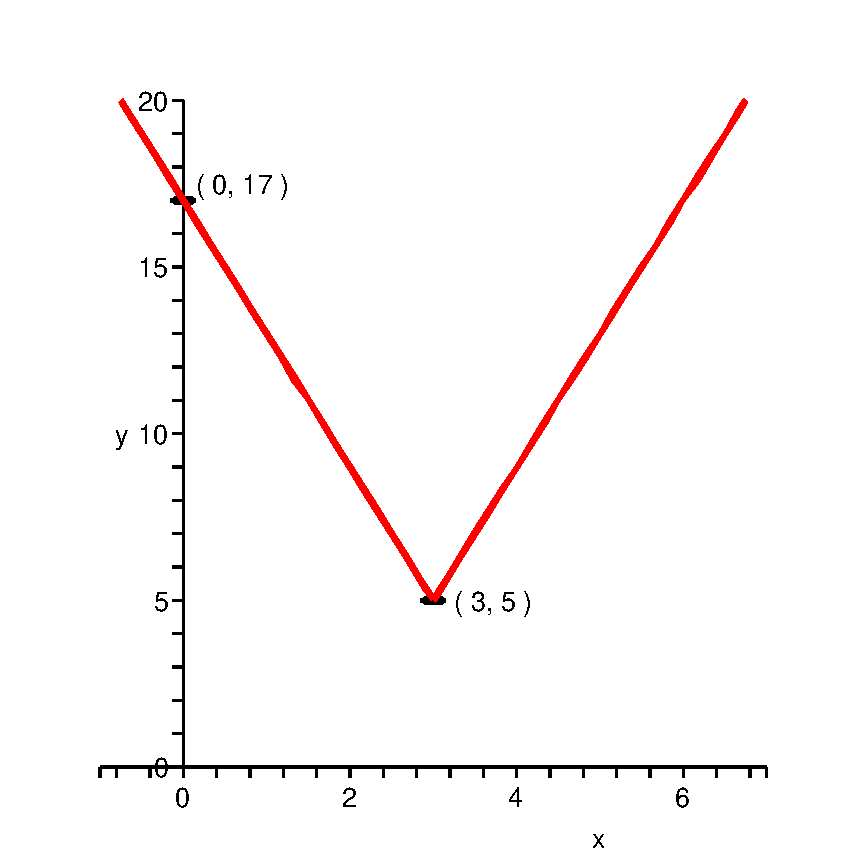
\includegraphics[width=8cm]{fonction1.eps}
 % fonction1.eps: 1048592x1048592 pixel, 0dpi\begin{center}
\end{center}
The \emph{y}-axis intercept is the value of \emph{f(x)} when $x=0$.
Here is the algebra:
\begin{eqnarray*}
f\left(0\right)
&=& 4\left\vert0-3\right\vert+5\\
&=& 4\left\vert-3\right\vert+5\\
&=& 4\times3+5\\
&=& 17
\end{eqnarray*}
Therefore, the answer is d$)$.\\


4004-- My savings are in an account at the bank. The evolution of
the total amount of money $A$ in my account increases with time $t$
(number of years) and is described by the following function :\\
$A = 5\,000\left(1.05\right)^{t}$.\\
How much money was there initially in my account?\\

R\'eponse : 5000\\

R\'etroaction :\\

We want to find the initial amount. Since $A$ increases as a
function of $t$ like $5\,000\left(1.05\right)^{x}$, the initial
amount is equal to the value of $A$ when $t$ is equal to 0.
\begin{eqnarray*}
A
&=& 5\,000\times\left(1.05\right)^{0}\\
&=& 5\,000\times1\\
&=& 5\,000
\end{eqnarray*}

The answer can also be read off the plot of the function $A=
5\,000\left(1,05\right)^{x}$.
\begin{center}
 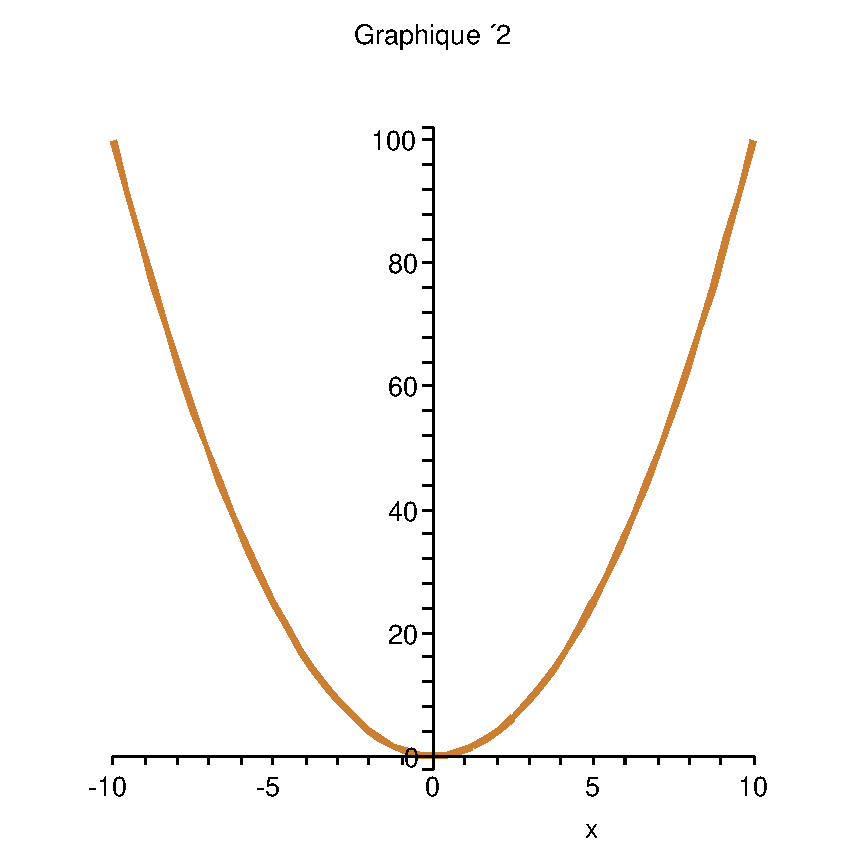
\includegraphics[width=13cm]{fonction4.eps}
 % fonction4.eps: 1048592x1048592 pixel, 0dpi\begin{center}
\end{center}
Therefore, the answer is $5,000$.\\


4006-- What are the zeros of the function plotted below?
\begin{center}
    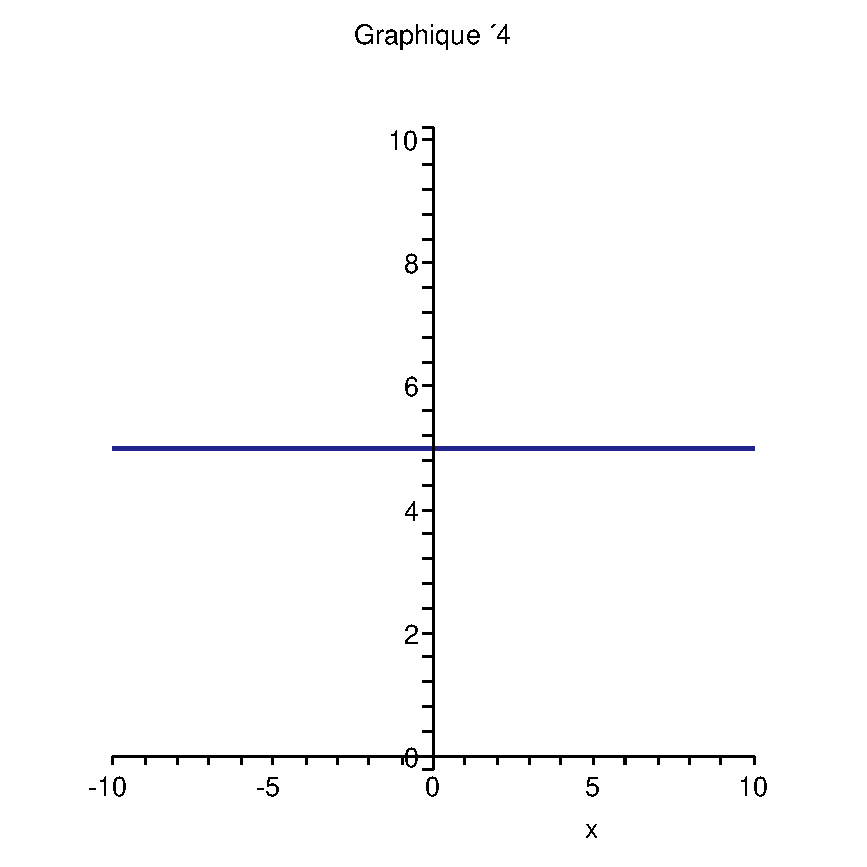
\includegraphics[width=8cm]{fonction6.eps}
% fonction6.eps : 300dpi, width=3.39cm, height=3.39cm, bb=0 0 400 400
    \end{center}

a$)$ $\nexists$\\
b$)$ $-\infty$\\
c$)$ $-\infty$ and $\infty$\\
d$)$ $+\infty$\\

R\'eponse : a$)$\\

R\'etroaction :\\

We want to find the zeros of the function plotted below.
\begin{center}
    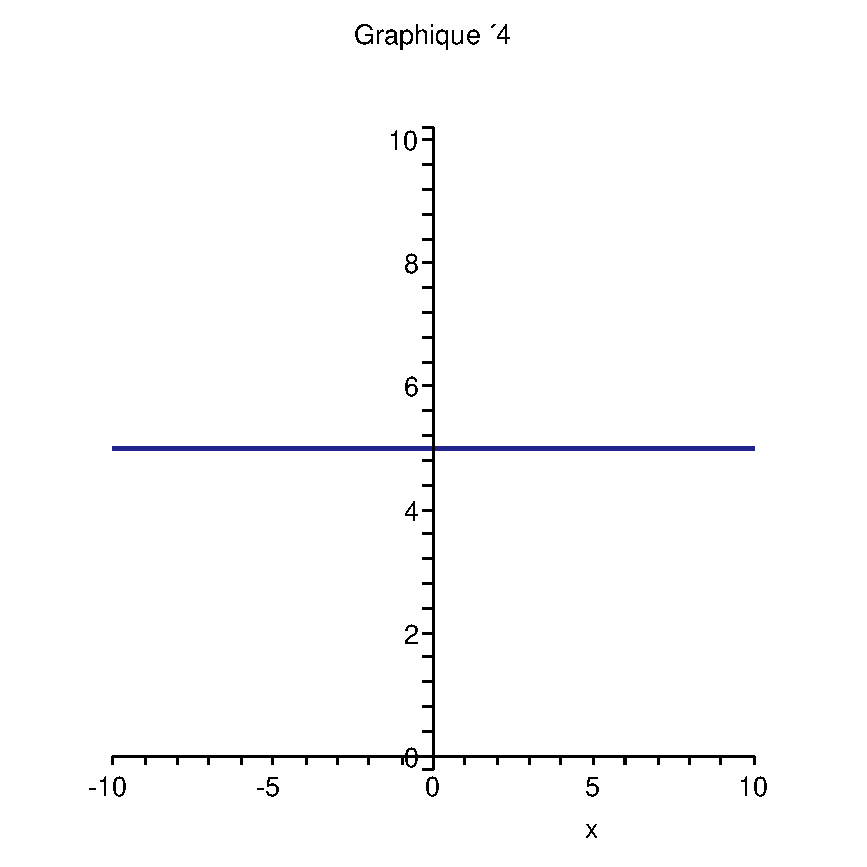
\includegraphics[width=8cm]{fonction6.eps}
% fonction6.eps : 300dpi, width=3.39cm, height=3.39cm, bb=0 0 400 400
    \end{center}
The zeros are the values of $x$ when $f\left(x\right)= 0$. Since
$f(x)$ is never equal to zero, the function does not have any zeros.\\
Therefore, the answer is a$)$.\\


4010-- Ann has a cellular phone and pays by the minute. If she
speaks 50 seconds, a full minute is charged. The first two minutes
of a call cost 0.30 \$ each and extra minutes cost 0.05 \$ each. The
price of calls as a function of duration is shown on the following
plot:

\begin{center}
    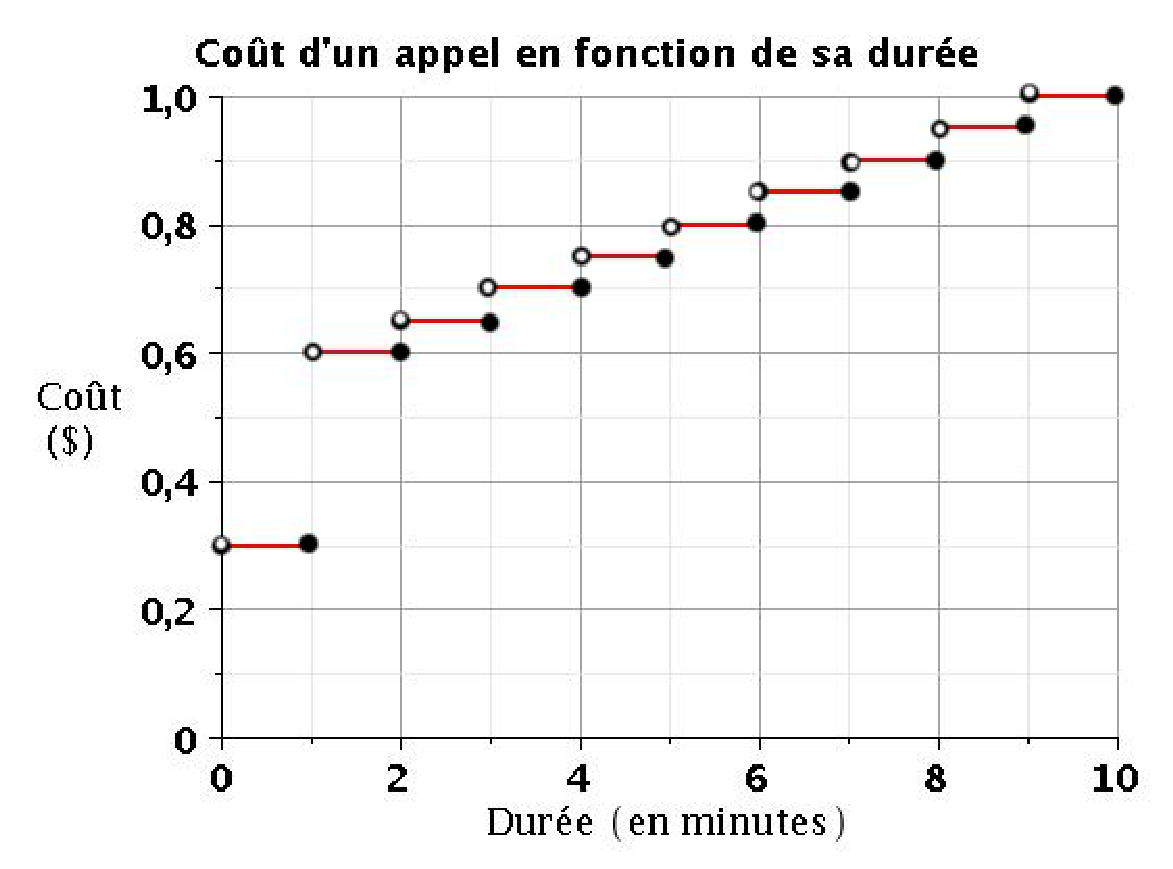
\includegraphics[width=12cm]{fonction10.eps}
% fonction10.eps : 300dpi, width=3.39cm, height=3.39cm, bb=0 0 400 400
    \end{center}
What are the possible prices for a call?\\

a$)$ All the multiples of 0.05 \$ and 0.3 \$.\\
b$)$ All the multiples of 0.05 over 0.55 \$, then 0.3 \$.\\
c$)$ All the multiples of 0.05 \$.\\
d$)$ All the multiples of 0.30 \$.\\

R\'eponse : b$)$\\

R\'etroaction :\\

\begin{center}
    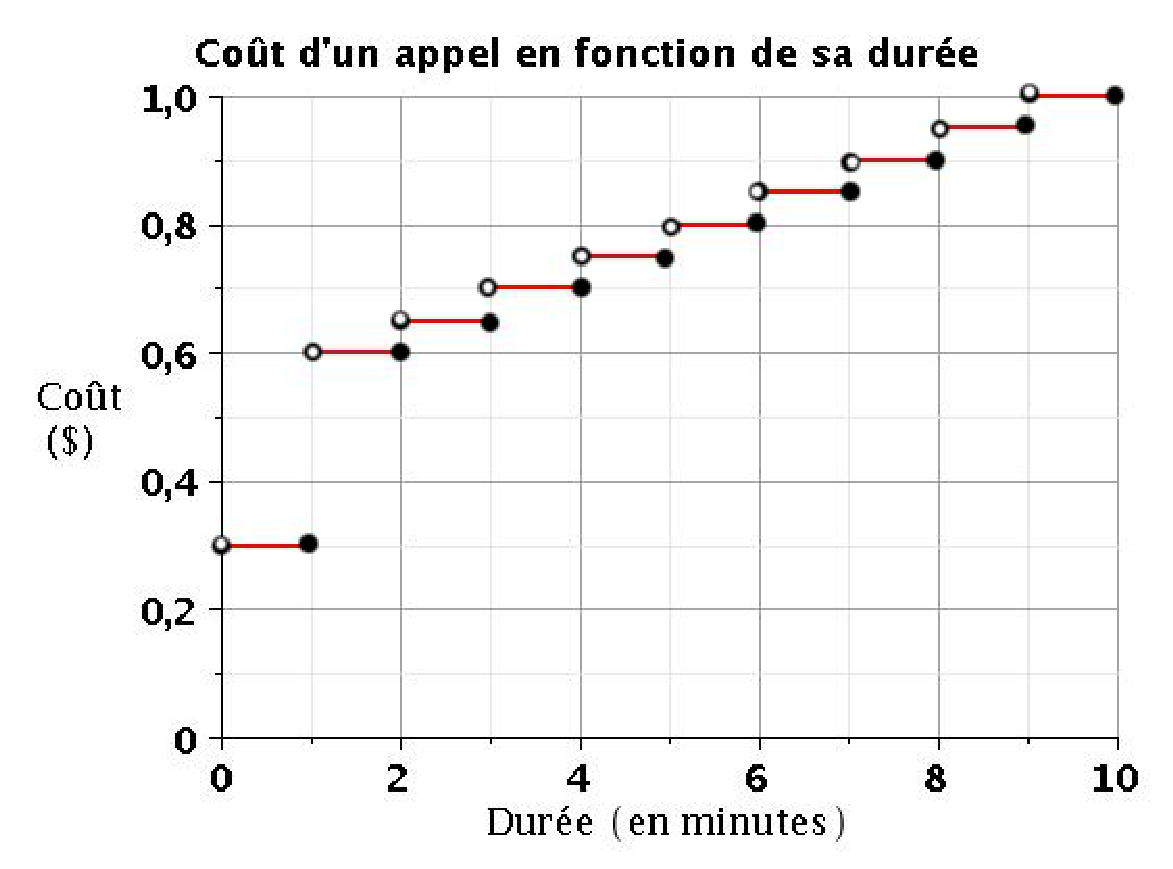
\includegraphics[width=12cm]{fonction10.eps}
% fonction10.eps : 300dpi, width=3.39cm, height=3.39cm, bb=0 0 400 400
    \end{center}

We are looking for the possible prices of a call. In fact, we need
to find the codomain of the function plotted or in other words, the
interval of its possible outputs. The codomain is
$\left\lbrace0,3,\,\, 0,6+0,05n\right\rbrace$,
where $n\, \epsilon\, \mathbb{N}$.\\
Therefore, the answer is b$)$.\\


4012-- What is the domain of the function $f\left(x\right)$?
\begin{center}
$f\left(x\right)=a \sqrt{x-h}+k$\\
\end{center}

a$)$ $]-\infty,\, h]$\\[2mm]
b$)$ $]-\infty,\, k]$\\[2mm]
c$)$ $[h, \,\infty[$\\[2mm]
d$)$ $[k,\,\infty[$\\

R\'eponse : c$)$\\

R\'etroaction :\\

We are looking for the domain of the function $f\left(x\right)=a
\sqrt{x-h}+k$. The domain is the interval of values that the
variable $x$ can take. The function is only defined when
$(x-h)\geqslant 0$.
thus, we have : $x\geqslant h$. The domain is $[h, \,\infty[$.\\
Therefore, the answer is c$)$.\\


4013-- Your friend opens the fridge to get some juice. The initial
temperature of the liquid is 4 degrees Celsius. He forgets the glass
of juice on the countertop. The liquid warms up following this rule:
\begin{center}
$f\left(x\right) = -17\left(\frac{1}{8}\right)^{x}+21$
\end{center}
\begin{center}
 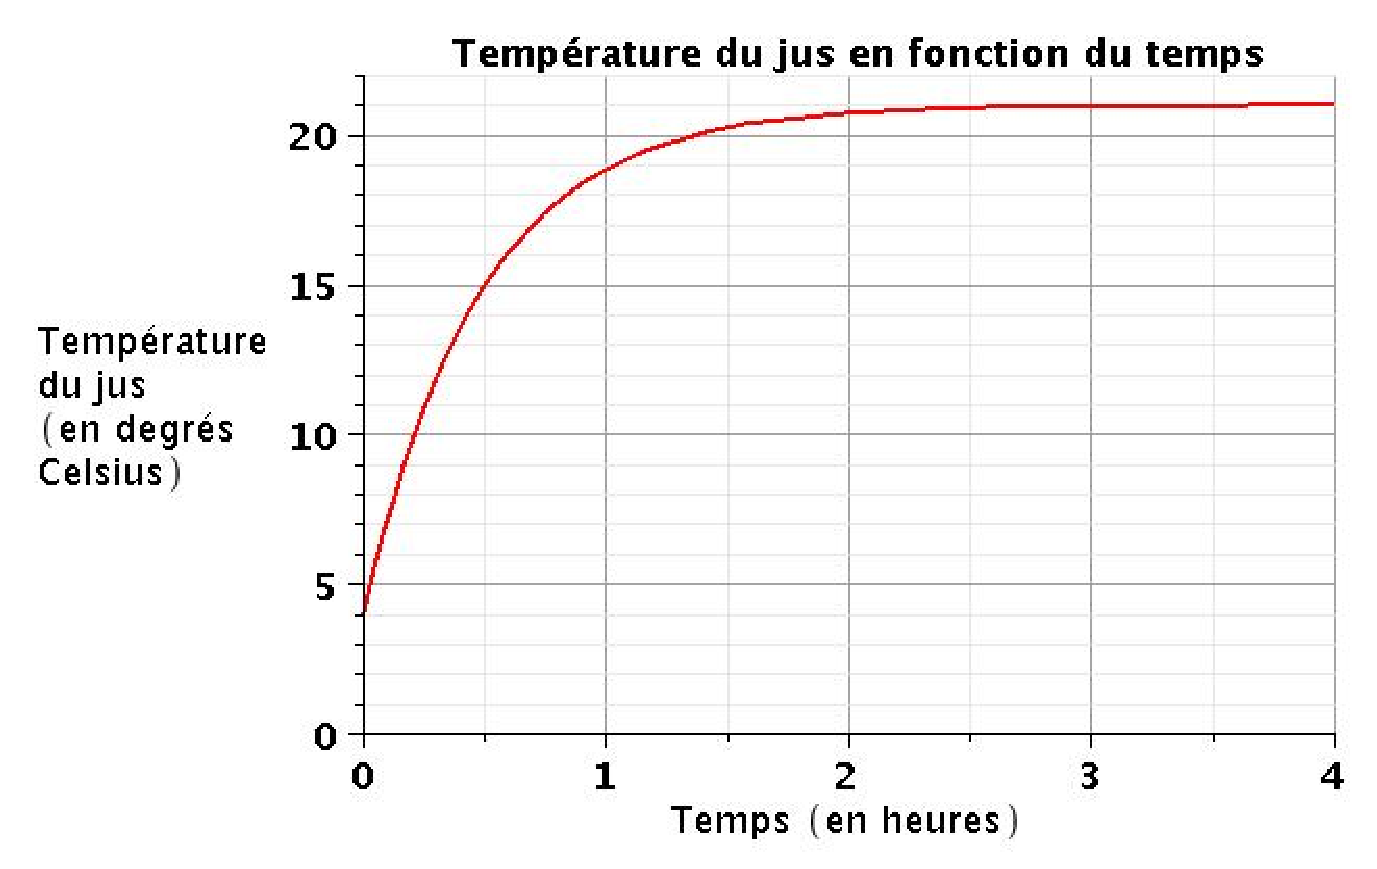
\includegraphics[width=13cm]{fonction13.eps}
 % fonction13.eps: 1048592x1048592 pixel, 0dpi\begin{center}
\end{center}
What is the temperature of the room the glass of juice is in?\\

R\'eponse : 21\\

R\'etroaction :\\

We are looking for the room temperature. The juice will warm up and
reach the room temperature after a very long time. To find the room
temperature, we find the supremum of the function $f\left(x\right) =
-17\left(\frac{1}{8}\right)^{x}+21$.
\begin{center}
 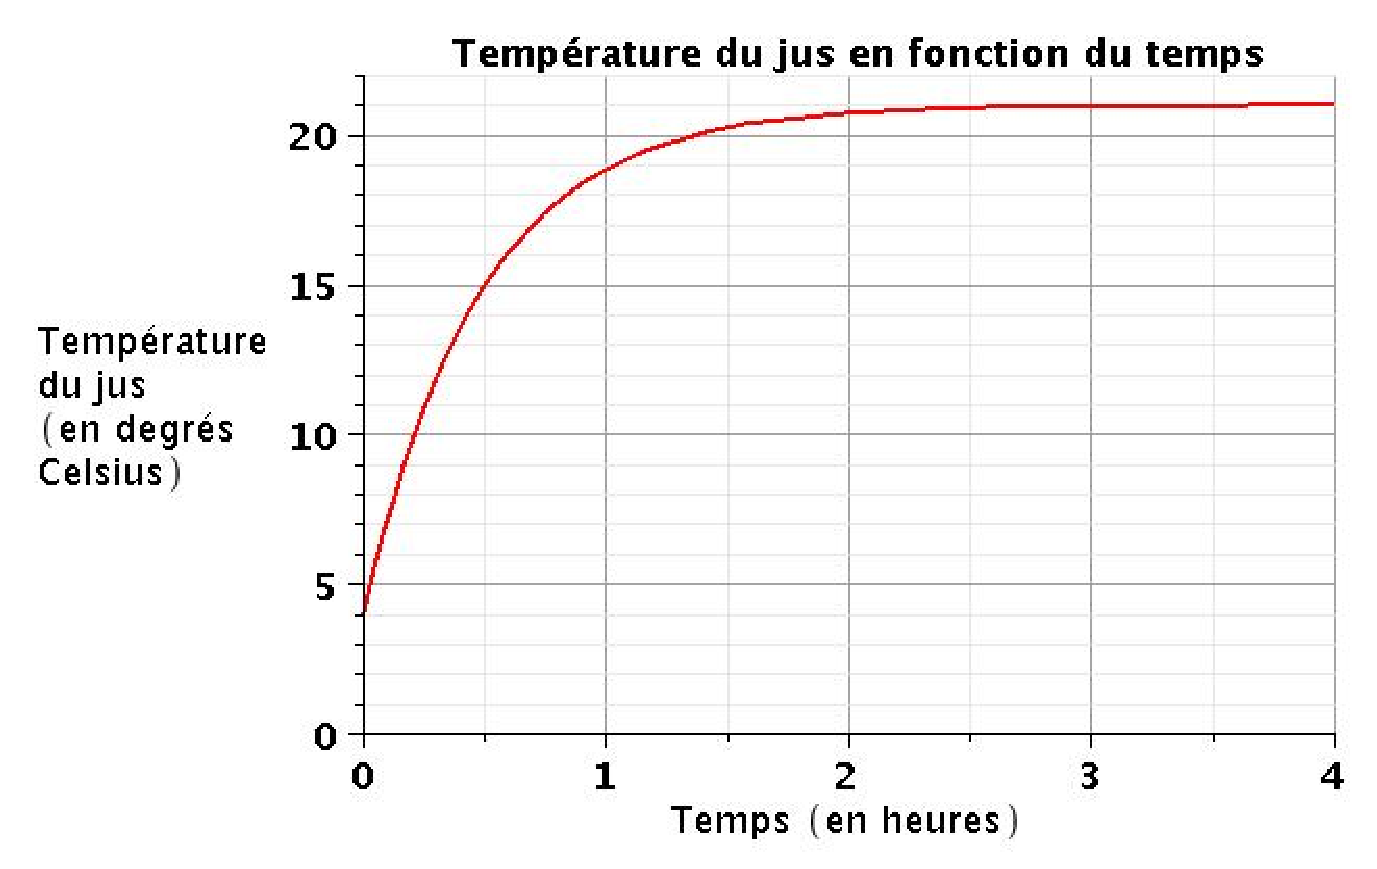
\includegraphics[width=13cm]{fonction13.eps}
 % fonction13.eps: 1048592x1048592 pixel, 0dpi\begin{center}
\end{center}
The codomain of the function $f(x)$ is $\left[4,21\right[$. The
supremum of this set is $21$. As you can see on the plot, the
function tends to $21$ as $x$ goes to infinity. In fact, as $x$ gets
larger, the term $\left(\frac{1}{8}\right)^{x}$ gets very close to
zero. In the limit when $x$ is very large, $f\left(x\right) =
-17\times 0+21 = 21$.\\
Therefore, the answer is $21$.\\


4016-- What is the codomain of the function?

\begin{center}
$f\left(x\right) = -4\left\vert x-2 \right\vert +5$
\end{center}

a$)$ $]-\infty,\, 5]$\\[2mm]
b$)$ $[5, \,\infty[$\\[2mm]
c$)$ $]-\infty,\, 2]$\\[2mm]
d$)$ $\mathbb{R}$\\

R\'eponse : a$)$\\

R\'etroaction :\\

Here is a plot of the function $f\left(x\right) = -4\left\vert x-2
\right\vert +5$ :
\begin{center}
 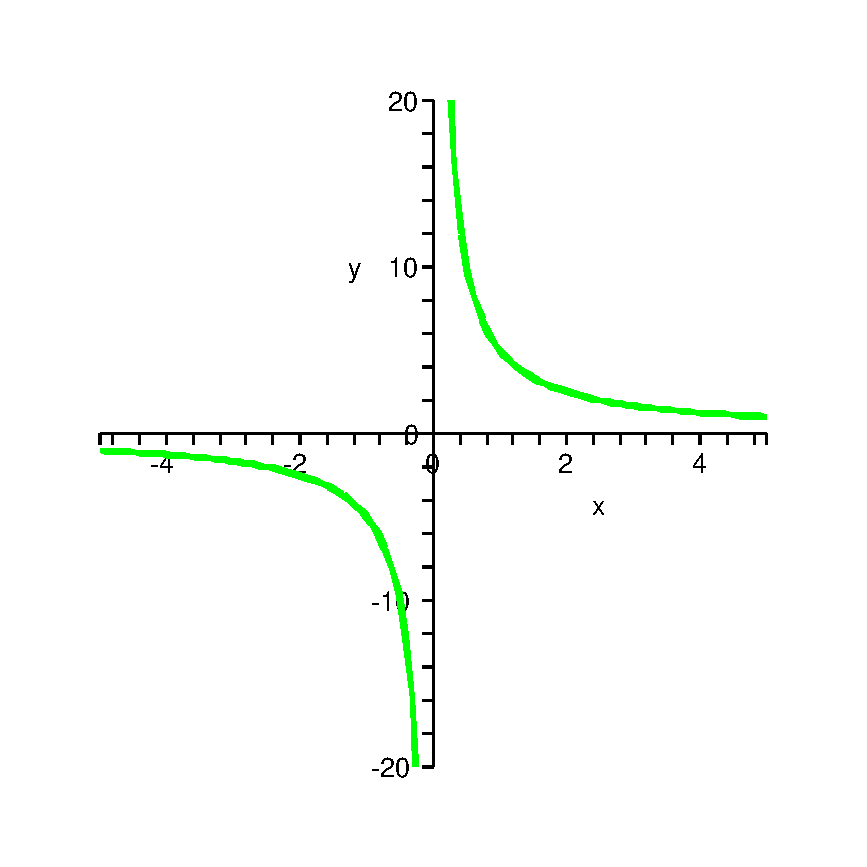
\includegraphics[width=8cm]{fonction16.eps}
 % fonction16.eps: 1048592x1048592 pixel, 0dpi\begin{center}
\end{center}
We are looking for the codomain of $f(x)$. The codomain of a
function is the set of all its possible outputs. The codomain of a
function of the type $f\left(x\right) = a\left\vert x-k \right\vert
+b$ is $]-\infty,\, k]$, if $a$ is negative. In this case $k$ is
equal to 2 and the codomain is $]-\infty,\, 5]$. The other answer
choices, $\mathbb{R}$ and $]-\infty,\, 2]$, correspond to the domain
and the interval of growth respectively.\\
The answer is $a)$.\\


4018-- Water slides have to be built at an aquatic park. The height
of a particular slide is described by the function
$h\left(x\right)=-\sqrt{4x}+6$, where $x$ is positive.
The units of $f(x)$ and $x$ are meters. How high is that slide?\\

R\'eponse : 6\\

R\'etroaction :\\

The height of the slide slide is described by the function
$h\left(x\right)=-\sqrt{4x}+6$ and the function is bounded in the first quadrant ($x$ is real).\\
Here is a plot:
\begin{center}
 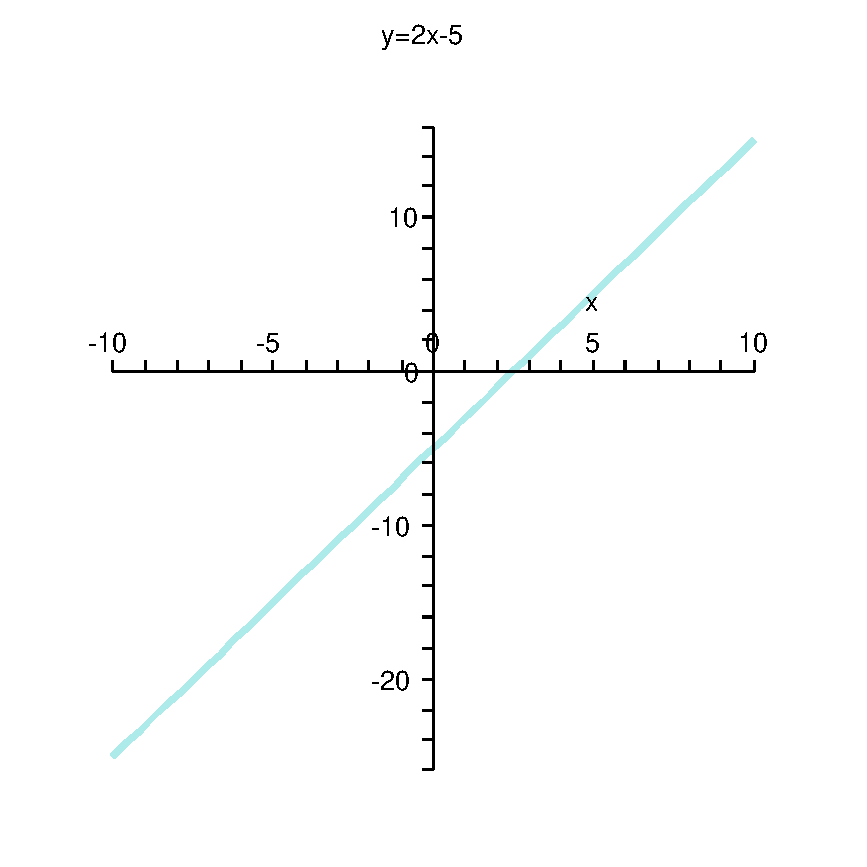
\includegraphics[width=8cm]{fonction18.eps}
 % fonction18.eps: 1048592x1048592 pixel, 0dpi\begin{center}
\end{center}
We are looking for the height of the slide. We have to find the span
of the codomain of $h(x)$, \emph{i.e.} the size of the interval of
values that $h\left(x\right)$ can give. The answer is $\left[0,\,
6\right]$. So, the top of the slides is six meters off the ground.
The slide is 6 meter high and the answer is $6$.\\


4019-- The intensity of the alternative current changes with time
like a sinusoidal function.
\begin{center}
$I\left(t\right)=100\sin\left(30\pi t\right)$
\end{center}
What is the range of amplitudes the current can take?\\

a$)$ $\left]-\infty,\, 100\right]$\\
b$)$ $\left[-100,\, 100\right]$\\
c$)$ $\left[-100,\, \infty\right[$\\
d$)$ $\mathbb{R}$\\

R\'eponse : b$)$\\

R\'etroaction :\\

The intensity of the alternative current changes with time like a
sine function.
\begin{center}
$I\left(t\right)=100\sin\left(30\pi t\right)$
\end{center}
Here is a plot:
\begin{center}
 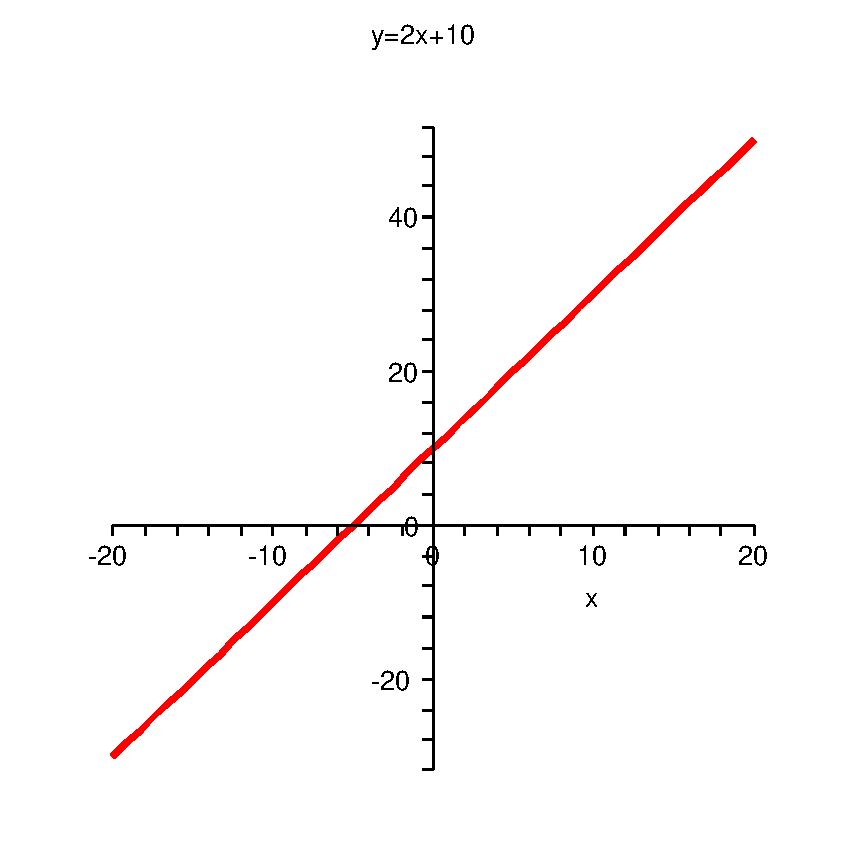
\includegraphics[width=8cm]{fonction19.eps}
 % fonction19.eps: 1048592x1048592 pixel, 0dpi\begin{center}
\end{center}
We need to know what values the function $I\left(t\right)$ can take, \emph{i.e.} its codomain.\\

As you can see on the plot, the function's minimum is -100 and its
maximum is 100.\\

In order to see this algebraically, you have to know that a sine
function of amplitude 1 takes values between -1 and 1. So with an
amplitude of 100 (without any vertical offset), our function ranges
from -100 to 100. Therefore, the codomain is $[-100, 100]$ and the answer is b$)$.\\


4020-- In chemistry, the acidity of substances is measured by a
quantity called $pH$. The pH is a function of hydrogen ions
concentration $x$, in moles per liter of solution and is determined
by the equation:
\begin{center}
$\textnormal{pH}=-\log(x)$
\end{center}
What values can the pH take if the concentration in moles per liter
ranges between $1\times10^{-14}$ and $0.1$?\\

a$)$ $\left]-\infty,\, 0\right]$\\
b$)$ $\left[0,\, \infty\right]$\\
c$)$ $\left[1,\, 14\right]$\\
d$)$ $\mathbb{R}$\\

R\'eponse : c$)$\\

R\'etroaction :\\

We want to find the range of values the pH can take, that is, the
codomain of the function $\textnormal{pH}=-\log(x)$. Since the
domain is bounded, so is the codomain. For a concentration of
$1\times10^{-14}$, the pH is $-\log(1\times10^{-14})=14$ and for a
concentration of $0.1$, the
pH is $-\log(0.1)=1$. So the codomain is $[1, 14]$.\\

Therefore, the answer is c$)$.\\


4024-- The surface area $A$ of a square can be found from its
perimeter $P$ with the function $A=(P/4)^{2}$. What function gives the value of the perimeter from the surface?\\

a$)$ $P=4\sqrt{A}$\\[2mm]
b$)$ $P=16\sqrt{A}$\\[2mm]
c$)$ $P=16A^{2}$\\[2mm]
d$)$ $P=256A^{2}$\\

R\'eponse : a$)$\\

R\'etroaction :\\

We are looking for an equation that gives the perimeter of a square
from the value of its surface. In other words, we want to inverse
the function $A=(P/4)^{2}$. We have to isolate the variable $P$.\\
Here is the algebra :\\
\begin{eqnarray*}
A &=& (P/4)^{2}\\
\sqrt{A} &=&(P/4) \\
4\sqrt{A} &=& P
\end{eqnarray*}
Therefore, the answer is a$)$.\\


4026-- Which function describes correctly the plot below?\\
\begin{center}
    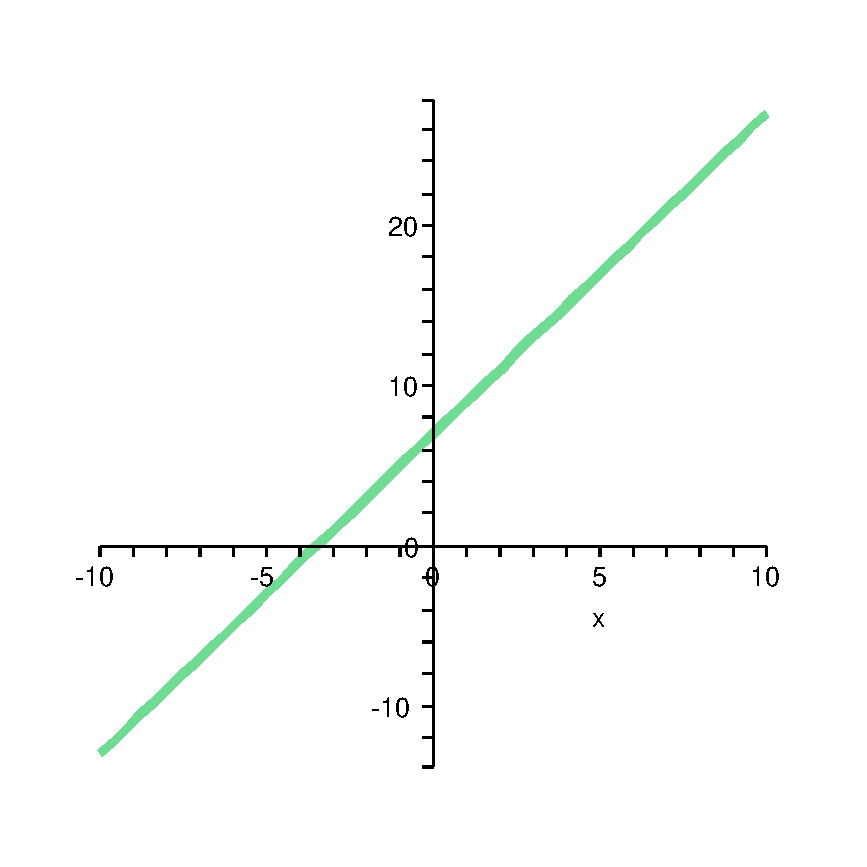
\includegraphics[width=8cm]{fonction26.eps}
% fonction26.eps : 300dpi, width=3.39cm, height=3.39cm, bb=0 0 400 400
    \end{center}

a$)$ $f\left(x\right) = -3\left\vert 4\left(x-\frac{5}{4}\right) \right\vert +15$\\[2mm]
b$)$ $f\left(x\right) = -3\left\vert 4x-\frac{5}{4} \right\vert +15$\\[2mm]
c$)$ $f\left(x\right) = 3\left\vert 4\left(x+\frac{5}{4}\right) \right\vert +15$\\[2mm]
d$)$ $f\left(x\right) = 3\left\vert 4x+5 \right\vert +15$\\

R\'eponse : a$)$\\

R\'etroaction :\\

We want to find the function represented on the plot below:
\begin{center}
    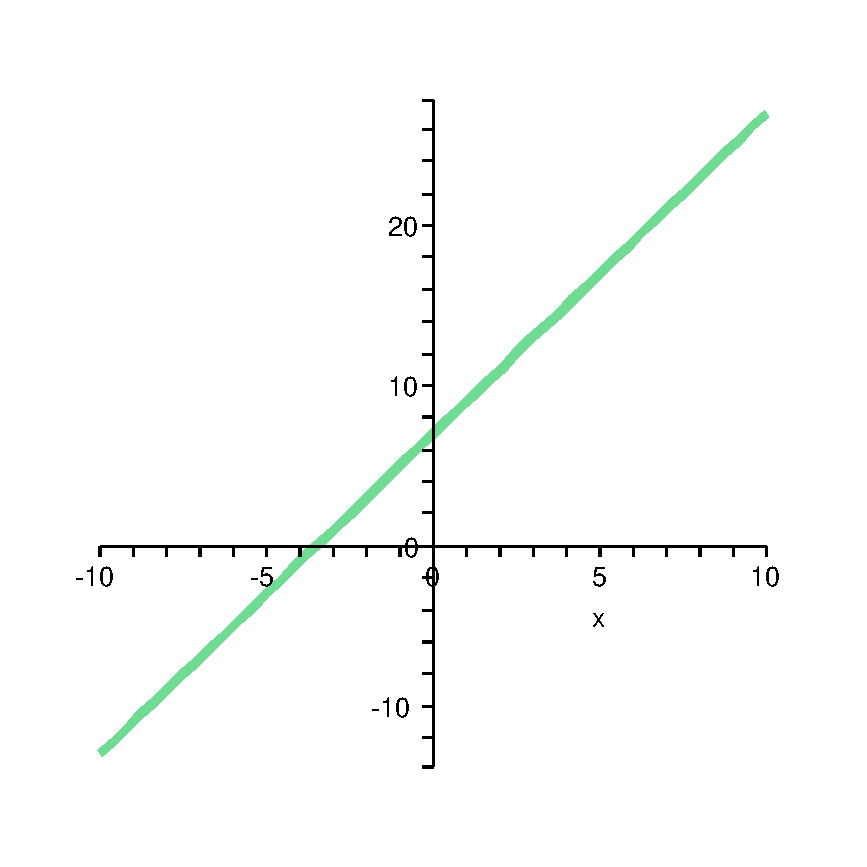
\includegraphics[width=8cm]{fonction26.eps}
% fonction26.eps : 300dpi, width=3.39cm, height=3.39cm, bb=0 0 400 400
    \end{center}
This is clearly a function of the form $f\left(x\right) =
a\left\vert bx+c \right\vert +d$. In this case, $a$ is negative and
$c$ = $+\frac{5}{4}$.\\[2mm]

The function $f(x) = -3\left\vert 4\left(x-\frac{5}{4}\right) \right\vert +15$ seems appropriate.\\[2mm]
The answer is a$)$.\\


4028-- The director of a great company wants to build a phone chain
to join the $10,000$ employees. He calls $5$ employees that each
call $5$ and so on. To visualize the chain, he wants to represent
the relationship between the group number of employees that are
calling and the number of people reached. The first group is made of
the director and the $5$ he's joining are the second group, so on.\\

True or false?\\
The function $f\left(x\right)=10\,000(5)^{x} $ represents the situation.\\

R\'eponse : False\\

R\'etroaction :\\

We are looking for the equation that rules the situation. The director joins $5$ employees who are joining $5$ people each, etc.\\
Here's a table that resumes.
\begin{center}
\begin{tabular}{ |l|l|}
\hline
Group number & Number of people reached\\
\hline
1 & 5\\
2 & 25\\
3 & 125\\
4 & 625\\
5 & 3125\\
\hline
\end{tabular}
\end{center}

When the group number increases by $1$, the number of people is $5$
times higher. So the equation is a base 5 exponential function. We
then have:
\begin{center}
$f\left(x\right)=5^{x}$
\end{center}
Therefore, the answer is : false.\\


4034-- During the spring, I empty my pool with a pump that has a
flow rate of four cubic meters an hour so I can fill it with clean
water using the same pump. My pool contains 54 cubic meter of water
when it is full and is two thirds full before being emptied in the
spring. How long will it take to empty the pool and how long to fill
it up?\\

a$)$ 4,5 hours and 9 hours\\
b$)$ 4,5 hours and 13,5 hours\\
c$)$ 9 hours and 13,5 hours\\
d$)$ 9 hours and 22,5 hours\\

R\'eponse : c$)$\\

R\'etroaction :\\

We are looking for the time to empty the pool and the time to fill it completely.\\
Because it contains 54 cubic meters when full and is filled to its
two third, it contains $\frac{2}{3}$ of $54 = 36$ cubic meters
before emptying in the spring. With $4$ cubic meters of flow rate,
the
time needed to empty the pool is:\\[2mm]
$\frac{36}{4}=9$\\

So the pool is empty after 9 hours. The time needed to fill it completely is:\\[2mm]
$\frac{54}{4}=13,5$\\

Therefore, the answer is c$)$.\\


4036-- Mark has decided to buy a brand new car. It costs $20\,000$
dollars. He wants to know what will be the reselling price $P$ of
the car in $x$ years knowing that the price changes with time
according to:

\begin{center}
$P=19\,500(0,85)^{x}+500$
\end{center}

True or false?\\
The rising interval of the function is $\left[0, \,\infty\right[$.\\

R\'eponse : False\\

R\'etroaction :\\

We are looking for the rising interval of the function
$P=19\,500(0,85)^{x}+500$. It is obvious on the graphic that the
function is decreasing over the interval $\left[0, \infty\right[$.
\begin{center}
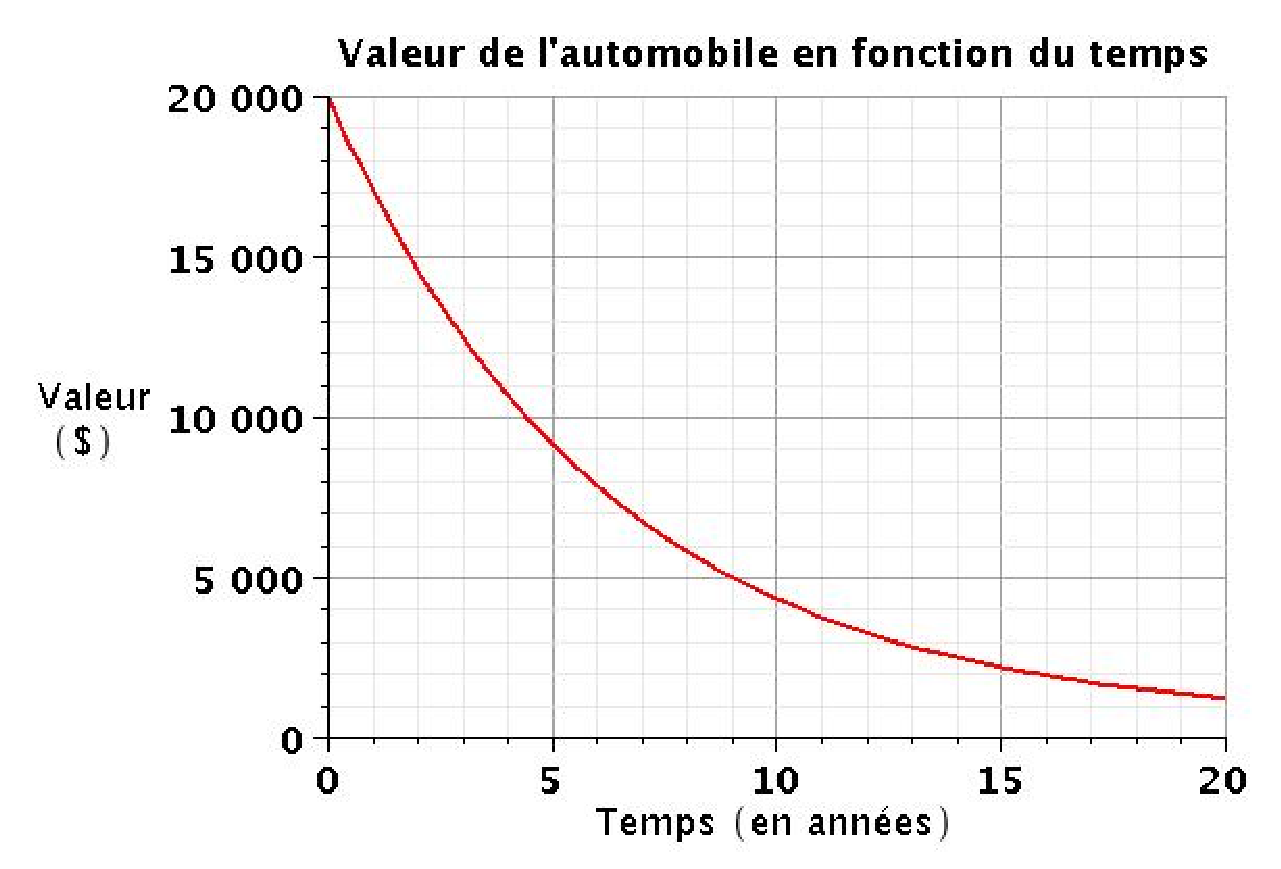
\includegraphics[width=10cm]{fonction36.eps}\\
% fonction36.eps : 300dpi, width=3.39cm, height=3.39cm, bb=0 0 400 400
\end{center}
We can also see with the canonical form of the function
$f\left(x\right)=ac^{b\left(x-h\right)}+k$ that the $c$ parameter of
the exponential function is less than $1$ and the $a$ parameter is
greater than $1$. So it is strictly decreasing and the interval
$\left[0, \infty\right[$ is then a decreasing one.\\
Therefore, the answer is : false.\\


4038-- Annie is studying bacteria. To do so, she needs at least
$100\,000$ bacteria. As the number of bacteria increases, a
relationship tells that number as a function of time in days:
\begin{center}
$f\left(x\right)=\log_{2}x$
\end{center}
How many days must pass before Annie has enough bacteria?\\

R\'eponse : 17\\

R\'etroaction :\\

When are looking for the time needed for Annie to have at least $100\,\,000$ bacteria.\\
We want to find $f\left(100\,\,000\right)$. Here's how to do it:
\begin{eqnarray*}
f\left(100\,000\right) &=& \log_{2}100\,000\\
f\left(100\,000\right) &=& \frac{\log 100\,000}{\log 2}\\
f\left(100\,000\right) &=& 16,61
\end{eqnarray*}

The graphic of the function also gives the answer.
\begin{center}
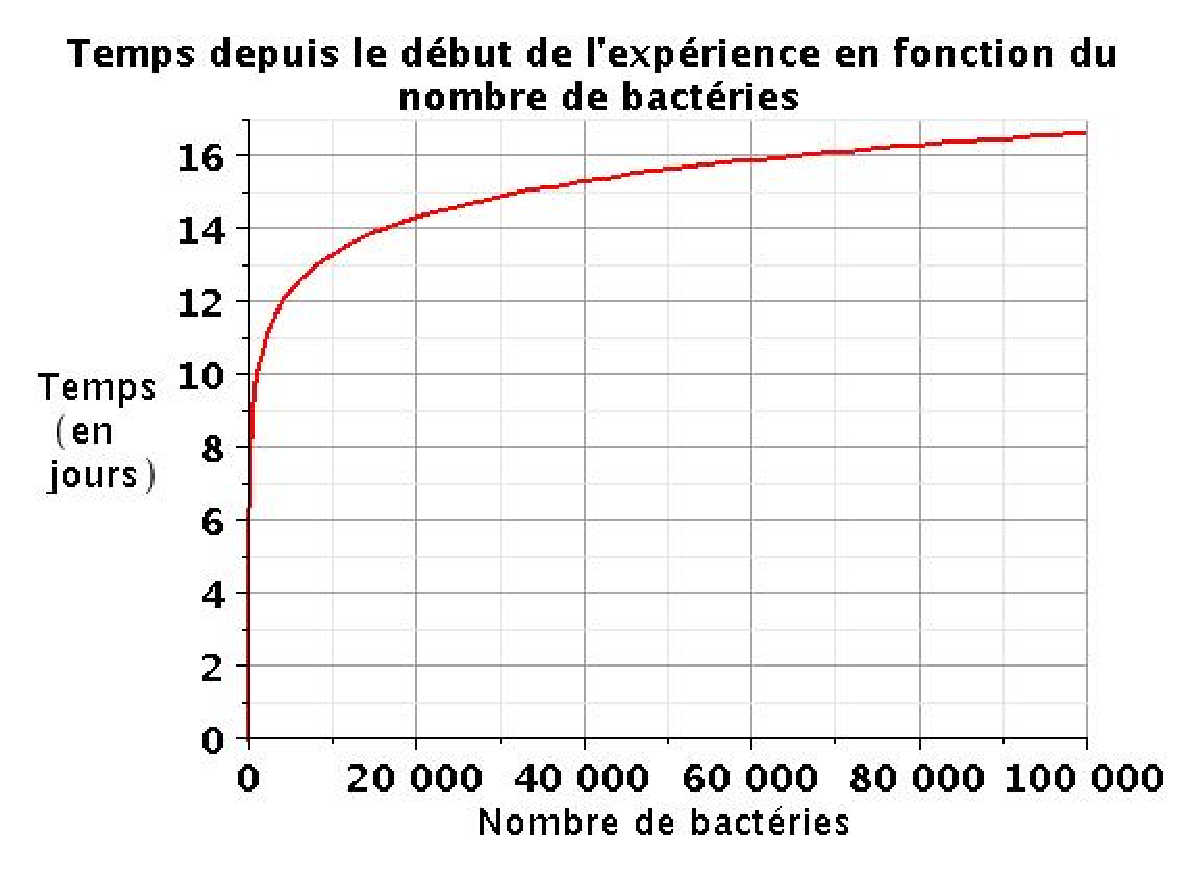
\includegraphics[width=10cm]{fonction38.eps}
% fonction38.eps : 300dpi, width=3.39cm, height=3.39cm, bb=0 0 400 400
\end{center}
Therefore, the answer is $17$.\\


4045-- My money is in a bank account. The amount $A$ is increasing
with time $x$ (in years) following that equation: $A=
5\,000\left(1,05\right)^{x}$. For how long has it been there so that
my profit is $6\,460$ dollars?\\

R\'eponse : 17\\

R\'etroaction :\\

We are looking for the number of years the amount has been in the
account so that the profit is $6\,460$ dollars. The amount $A$
increases with $x$, in years, following $A=
5000\left(1,05\right)^{x}$.\\ If the profit is $6\,460$ dollars, the
final amount is $5\,000+6\,460=11\,460$ dollars. Then place the
amount in the equation and isolate $x$ in order to find it.
\begin{eqnarray*}
11\,460 &=& 5\,\,000\times\left(1,05\right)^{x}\\
\frac{11\,460}{5\,\,000} &=& \left(1,05\right)^{x}\\
\frac{573}{250} &=& \left(1,05\right)^{x}\\
\log_{1,05}\left(\frac{573}{250}\right) &=& x\\
17 &=& x
\end{eqnarray*}

The answer can also be found on the graphic of the function $A=
5000\left(1,05\right)^{x}$.
\begin{center}
 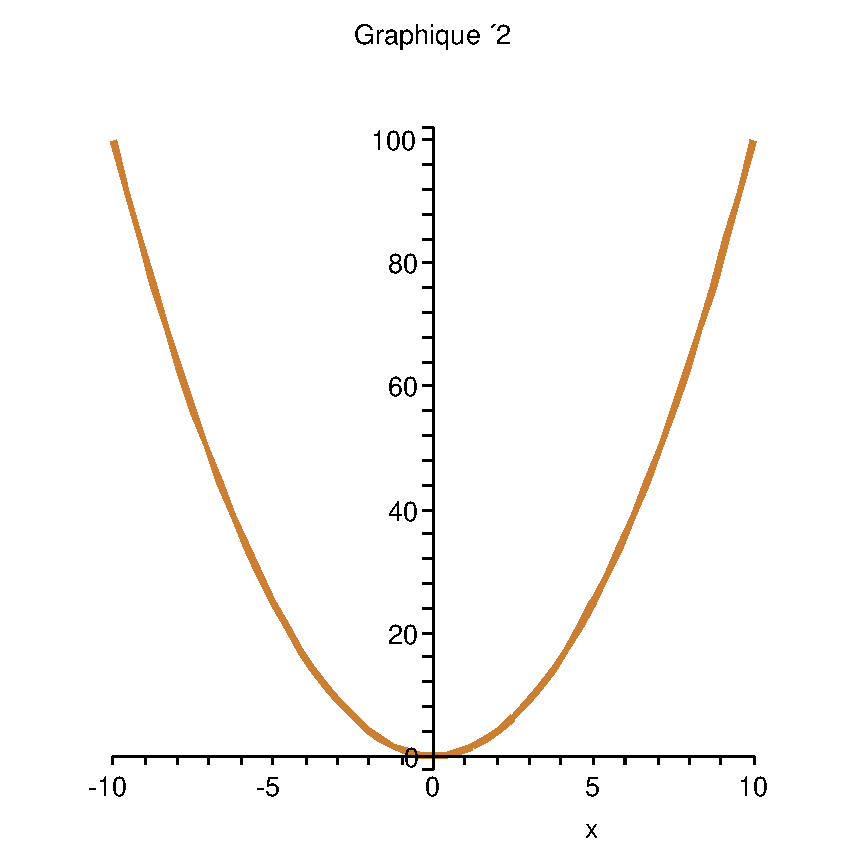
\includegraphics[width=12cm]{fonction4.eps}
 % fonction4.eps: 1048592x1048592 pixel, 0dpi\begin{center}
\end{center}
Therefore, the answer is $17$.\\


4047-- For what values of $x$ is the following function positive?
\begin{center}
 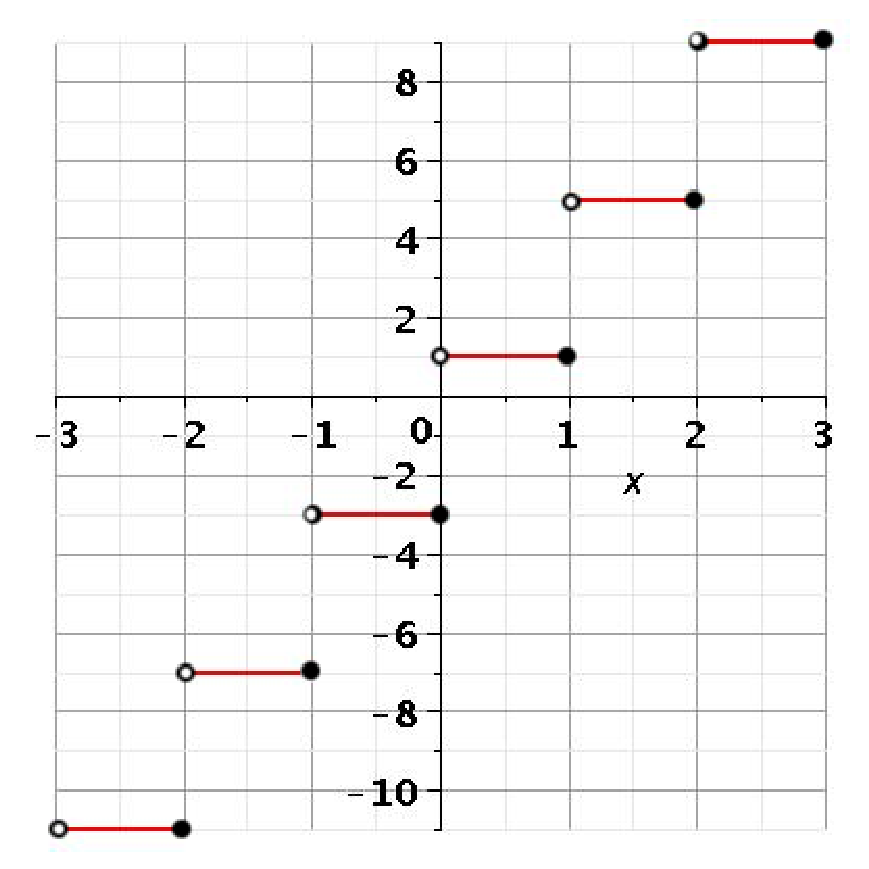
\includegraphics[width=8cm]{fonction17.eps}
 % fonction17.eps: 1048592x1048592 pixel, 0dpi\begin{center}
\end{center}

a$)$ $-11$, $-7$ and $-3$\\
b$)$ $1$, $5$ and $9 $\\
c$)$ $\left]-\infty,\, 0\right]$\\
d$)$ $\left]0, \,\infty\right[$\\

R\'eponse : d$)$\\

R\'etroaction :\\

We are looking for a range of values of $x$ so that the function is
positive.
\begin{center}
 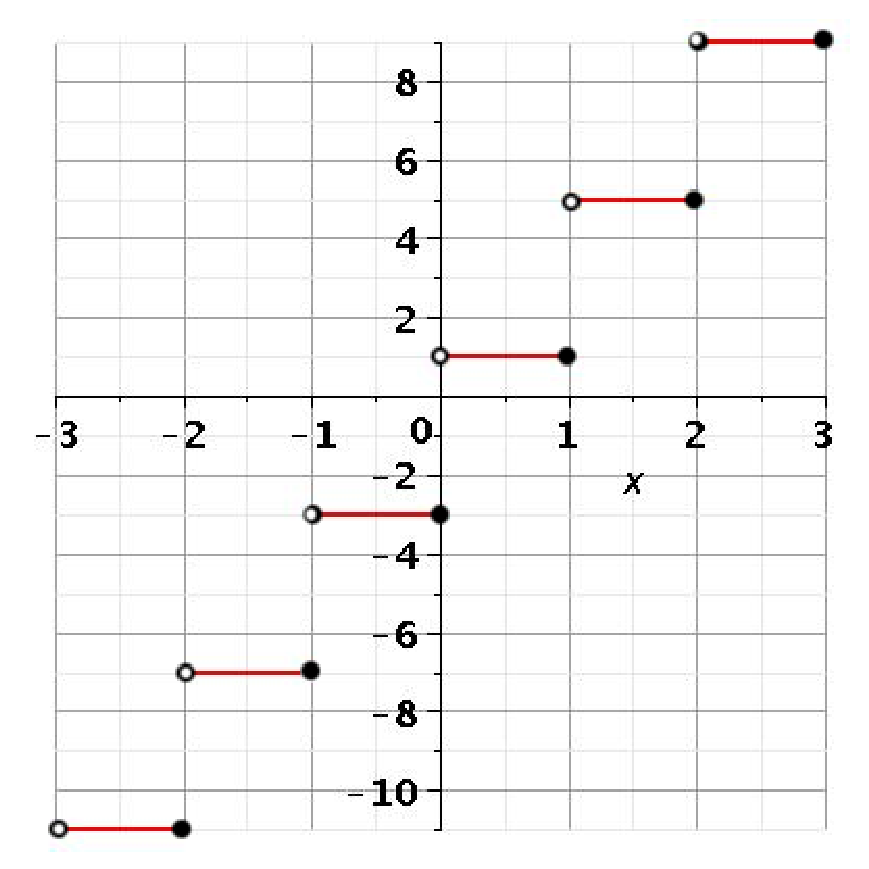
\includegraphics[width=8cm]{fonction17.eps}
 % fonction17.eps: 1048592x1048592 pixel, 0dpi\begin{center}
\end{center}
So we want $y\geq0$. It is obvious on the graphic that $y\geq0$ if
$x>0$. The range of interest is then $\left]0,\, \infty\right[$.\\
Therefore, the answer is d$)$.\\


4052-- On a nice Saturday, the temperature between 7am and 5pm
varies according to the graphic. I was outdoor hiking between 9am
and 4pm. At what time was it the hottest?
\begin{center}
    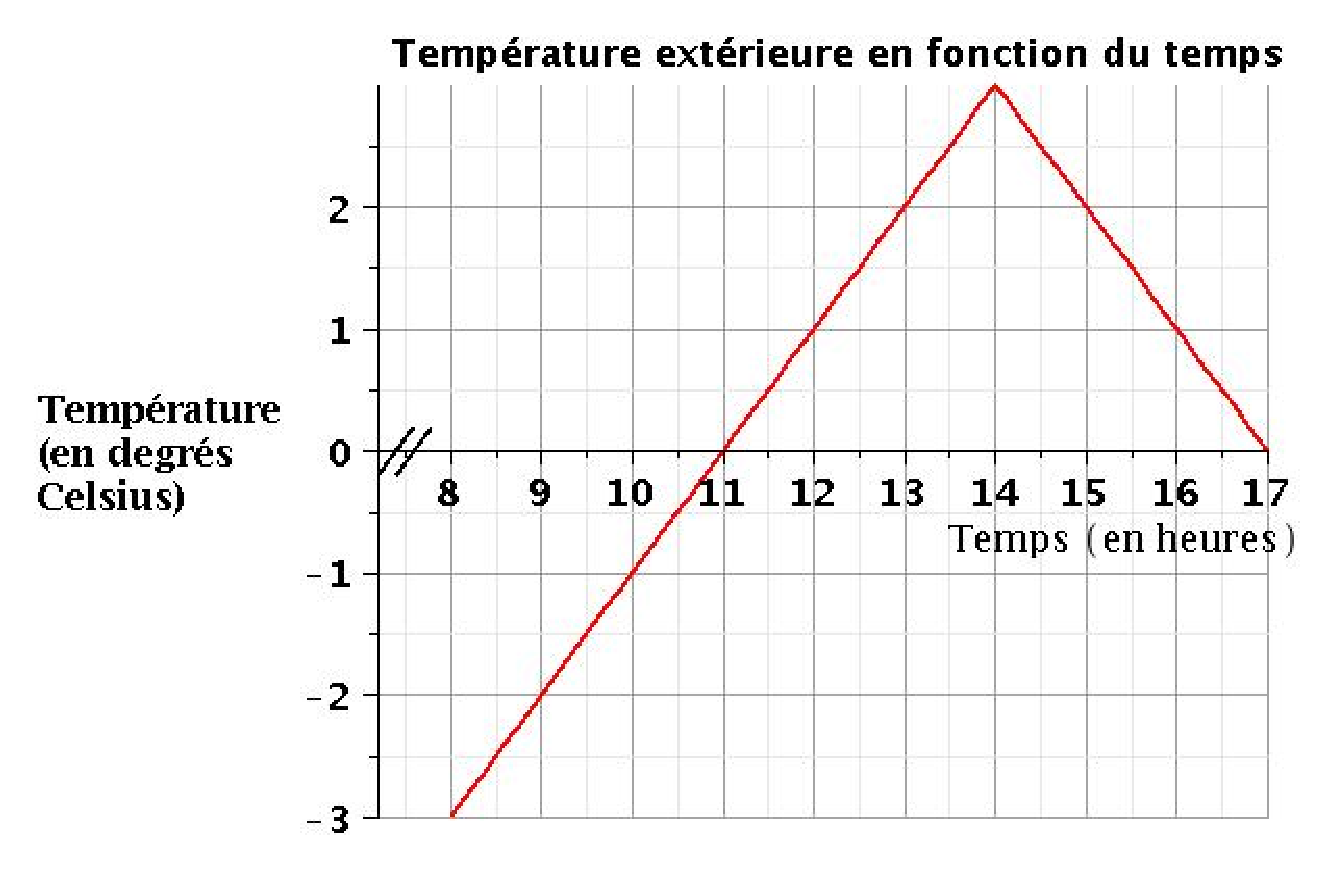
\includegraphics[width=12cm]{fonction44.eps}
% fonction44.eps : 300dpi, width=3.39cm, height=3.39cm, bb=0 0 400 400
    \end{center}

R\'eponse : 2pm\\

R\'etroaction :\\

We are looking for the time at which the temperature curve is
peaking.
\begin{center}
    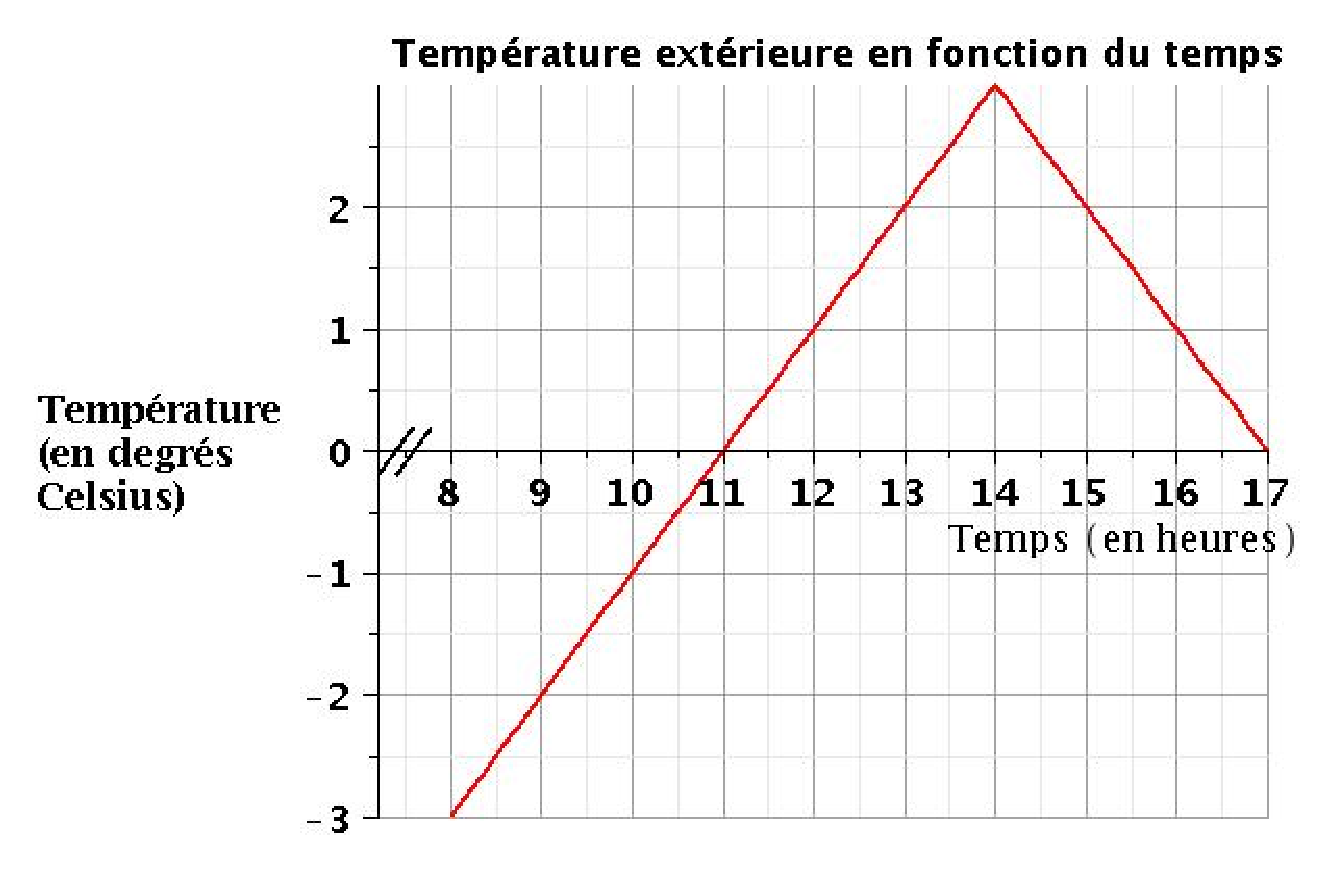
\includegraphics[width=12cm]{fonction44.eps}
% fonction44.eps : 300dpi, width=3.39cm, height=3.39cm, bb=0 0 400 400
    \end{center}
The maximum is 3 degrees Celsius and occurs at 2pm.\\
Therefore, the answer is $2pm$.\\


4054-- Mark has decided to buy a brand new car. It costs $20\,000$
dollars. He wants to know what will be the reselling price $P$ of
the car in $x$ years knowing that the price changes with time
according to:

\begin{equation*}
f\left(x\right)=a(0,85)^{x}+k
\end{equation*}

After two years, the car is worth  $14\,588,75$ dollars.


What will be the minimal value of the car?\\

R\'eponse : $500\,\$$\\

R\'etroaction :\\

We are looking for the lowest price the car will get to with time,
that is, the minimum of the function. The $k$ parameter of the
canonical form is the answer.\\
The function is of the form $f\left(x\right)=a(0,85)^{x}+k$.
Moreover, we know two points: $\left(0,\,20\,000\right)$ and
$\left(2,\,14\,588,75\right)$. With those put in the function, the
$a$ and $k$ parameters will be found. We have:
\begin{eqnarray*}
20\,000 &=& a(0,85)^{0}+k\\
20\,000 &=& a(1)+k\\
20\,000-a &=& k
\end{eqnarray*}
and
\begin{eqnarray*}
14\,588,75 &=& a(0,85)^{2}+k\\
14\,588,75 &=& a(0,7225)+k\\
14\,588,75-0,7225a &=& k
\end{eqnarray*}
So by comparing:
\begin{eqnarray*}
20\,000-a &=& 14\,588,75-0,7225a\\
5\,411,25 &=& 0,2775a\\
\frac{5\,411,25}{0,2775} &=& a\\
19\,500= a
\end{eqnarray*}
and by substitution,
\begin{eqnarray*}
20\,000-a &=& k\\
20\,000- 19\,500 &=& k\\
500 &=& k
\end{eqnarray*}
The function is then represented by:
\begin{center}
$f\left(x\right)=19\,500(0,85)^{x}+500$
\end{center}
\begin{center}
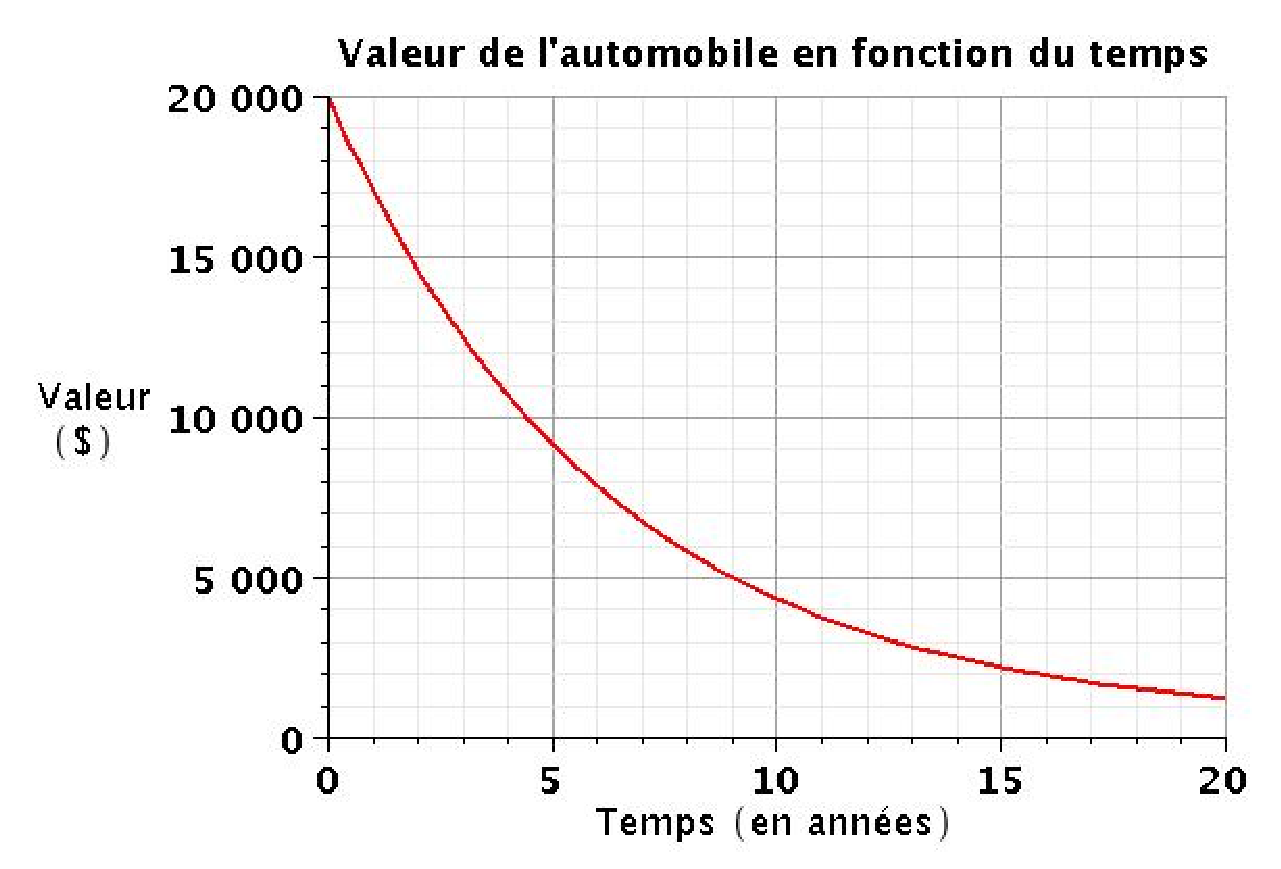
\includegraphics[width=12cm]{fonction36.eps}
% fonction36.eps : 300dpi, width=3.39cm, height=3.39cm, bb=0 0 400 400
\end{center}
So the lowest value of the car is the $k$ parameter, $500$ dollars.\\
Therefore, the answer is $500$ dollars.\\


4056-- The number of hours of enlightenment changes to the days of
the year. This variation is ruled in a particular region by the
following equation:
\begin{center}
$f\left(x\right)=4\sin \frac{2\pi}{365}(x-91,25)+12$.
\end{center}

What are the lowest and highest amounts of enlightenment for a day in that region?\\

a$)$ 4 hours and 8 hours\\
b$)$ 4 hours and 16 hours\\
c$)$ 8 hours and 16 hours\\
d$)$ 12 hours and 16 hours\\

R\'eponse : c$)$\\

R\'etroaction :\\

The number of hours of enlightenment is ruled by the following
equation:
\begin{center}
$f(x)=4\sin \frac{2\pi}{365}(x-91,25)+12$.
\end{center}

We are looking for the maximum and the minimum of the function.
Because it oscillates around $y=12$ and the amplitude is $4$, the
maximum is $12$ hours $+ 4$ hours $= 16$ hours and the minimum is $12$ hours $- 4$ hours $= 8$ hours.\\
The graphic also gives that information.
\begin{center}
    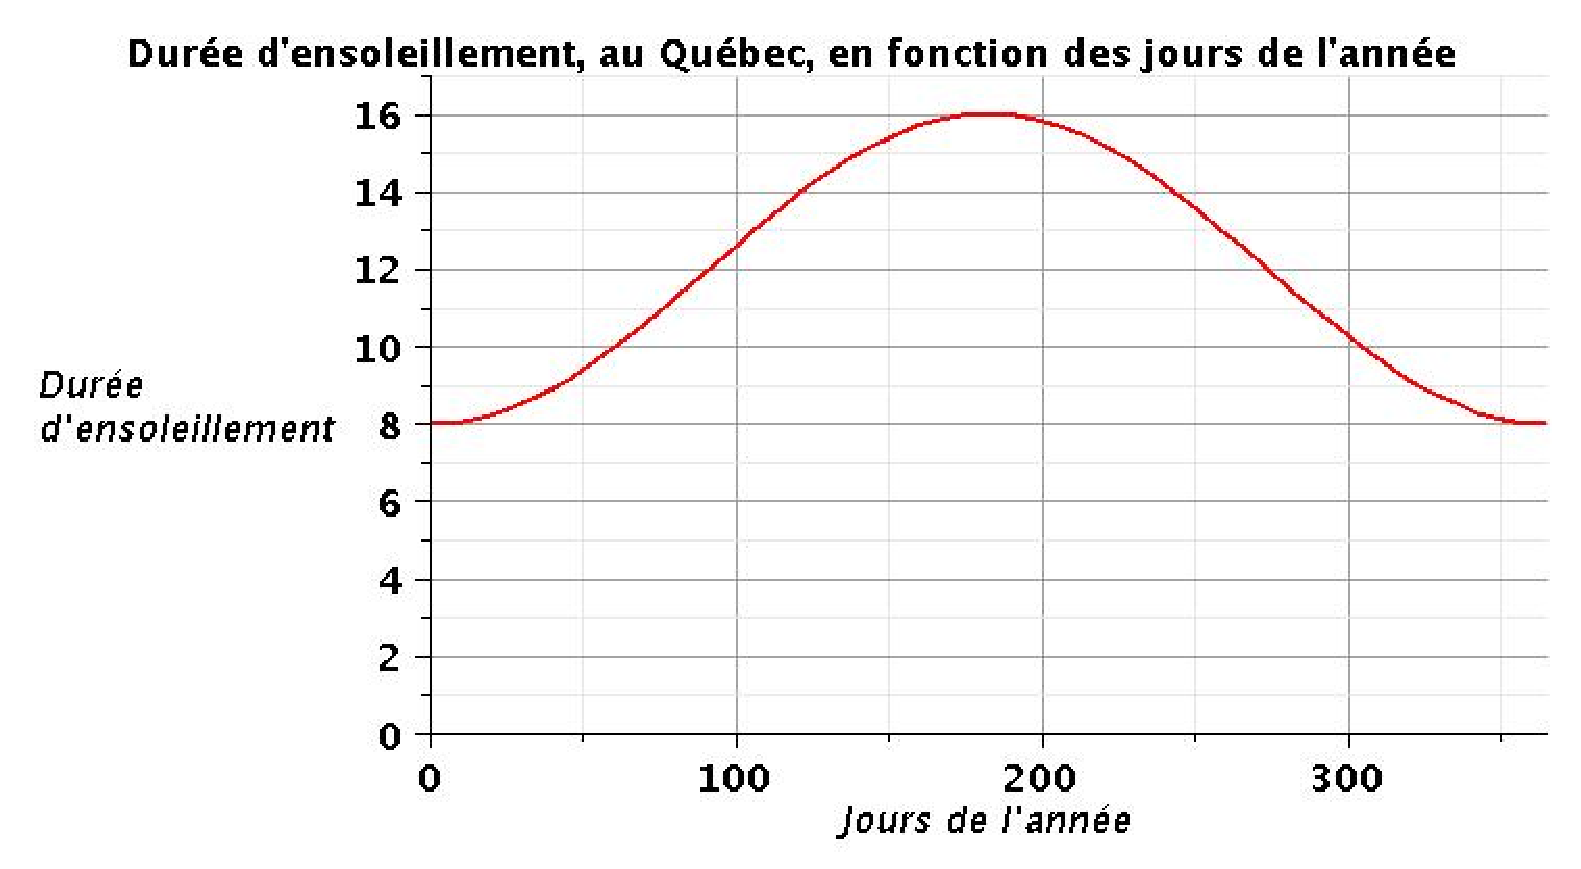
\includegraphics[width=12cm]{fonction56.eps}
% fonction53.eps : 300dpi, width=3.39cm, height=3.39cm, bb=0 0 400 400
    \end{center}
Therefore, the answer is c$)$.\\

4057-- What am I?\\
I have an asymptote at $x=-1$ and I am decreasing over my entire domain.\\

a$)$ $f\left(x\right)=\frac{x^2+x-2}{x^2-1}$\\[2mm]
b$)$ $f\left(x\right)=\frac{x+4}{x-1}$\\[2mm]
c$)$ $f\left(x\right)=\log\left(-x\right)-1$\\[2mm]
d$)$ $f\left(x\right)=\log\left(x+1\right)$\\[2mm]

R\'eponse : a$)$\\

R\'etroaction :\\

We are looking for the function that has an asymptote at $x=-1$ and
that is decreasing over its entire domain
from the following:\\

a$)$ $f\left(x\right)=\frac{x^2+x-2}{x^2-1}$\\[2mm]
b$)$ $f\left(x\right)=\frac{x+4}{x-1}$\\[2mm]
c$)$ $f\left(x\right)=\log\left(-x\right)-1$\\[2mm]
d$)$ $f\left(x\right)=\log\left(x+1\right)$\\[2mm]

The function a$)$ can be simplified.
\begin{eqnarray*}
f\left(x\right) &=& \frac{x^2+x-2}{x^2-1}\\
&=& \frac{\left(x-1\right)\left(x+2\right)}{\left(x-1\right)\left(x+1\right)}\\
&=& \frac{\left(x+2\right)}{\left(x+1\right)}\\
&=& \frac{x+2}{x+1}\\
&=& 1 + \frac{1}{x+1}
\end{eqnarray*}
That function fulfills the conditions.\\
\begin{center}
    \includegraphics[width=8cm]{fonction57.eps}
% fonction57.eps : 300dpi, width=3.39cm, height=3.39cm, bb=0 0 400 400
    \end{center}
The function b$)$ has $x=1$ as asymptote.\\
The function c$)$ has $x=0$ as asymptote.\\
The function d$)$ is increasing.\\
Therefore, the answer is a$)$.\\

4058-- What am I?\\
I always have only one zero and I don't have any asymptotes.\\

a$)$ A straight line: $f\left(x\right) = ax+b$\\
b$)$ A logarithmic function: $f\left(x\right) = a\log_c b\left(x-h\right)+k$\\
c$)$ A square root function: $f\left(x\right) = a\sqrt{b\left(x-h\right)}+k$\\
d$)$ An absolute value function: $f\left(x\right) = a|b\left(x-h\right)|+k$\\

R\'eponse : a$)$\\

R\'etroaction :\\

We are looking for a function that always has only one zero and that has no asymptote, from those:\\

a$)$ A straight line: $f\left(x\right) = ax+b$\\
b$)$ A logarithmic function: $f\left(x\right) = a\log_c b\left(x-h\right)+k$\\
c$)$ A square root function: $f\left(x\right) = a\sqrt{b\left(x-h\right)}+k$\\
d$)$ An absolute value function: $f\left(x\right) = a|b\left(x-h\right)|+k$\\

The functions that always have only one zero are the straight lines
and the logarithmic functions. The straight line has no asymptote
while the log function does. So the function we are looking for is a
straight
line.\\
Therefore, the answer is a$)$.\\

4059-- What am I?\\
I always have only one zero and my domain is never the entirety of
the real numbers.\\

a$)$ A straight line: $f\left(x\right) = ax+b$\\
b$)$ An exponential function: $f\left(x\right) = ac^{b\left(x-h\right)}+k$\\
c$)$ A logarithmic function: $f\left(x\right) = a\log_c b\left(x-h\right)+k$\\
d$)$ A square root function: $f\left(x\right) = a\sqrt{b\left(x-h\right)}+k$\\

R\'eponse : c$)$\\

R\'etroaction :\\

We are looking for a function that always has only one zero and that
the domain is never the entirety of the real numbers:\\

a$)$ A straight line: $f\left(x\right) = ax+b$\\
b$)$ An exponential function: $f\left(x\right) = ac^{b\left(x-h\right)}+k$\\
c$)$ A logarithmic function: $f\left(x\right) = a\log_c b\left(x-h\right)+k$\\
d$)$ A square root function: $f\left(x\right) = a\sqrt{b\left(x-h\right)}+k$\\

The functions that always have only one zero are the straight lines
and the logarithmic functions. The straight line is always defined
over the real numbers entirely, opposed to the log functions that
aren't. So the function we are looking for is the logarithmic function.\\
Therefore, the answer is c$)$.\\


4060-- What am I?\\
My codomain always corresponds to an interval like this one:
$\left]-\infty, \,a\right]$ or
$\left[a,\, \infty\right[$\quad where\quad$a\,\epsilon\,\mathbb{R}$.\\
I sometimes don't have any zeros and sometimes I have one or two.\\

a$)$ An exponential function: $f\left(x\right) = ac^{b\left(x-h\right)}+k$\\
b$)$ A highest integer function: $f\left(x\right) = a[b\left(x-h\right)]+k$\\
c$)$ A square root function: $f\left(x\right) = a\sqrt{b\left(x-h\right)+k}$\\
d$)$ An absolute value function: $f\left(x\right) = a|b\left(x-h\right)|+k$\\

R\'eponse : d$)$\\

R\'etroaction :\\

We are looking for a function that can have none, 1 or 2 zeros and
its codomain is always an interval of the form: $\left]-\infty,
\,a\right]$ or $\left[a,\, \infty\right[$\quad where\quad$a\,\epsilon\,\mathbb{R}$ from the following:\\

a$)$ An exponential function: $f\left(x\right) = ac^{b\left(x-h\right)}+k$\\
b$)$ A highest integer function: $f\left(x\right) = a[b\left(x-h\right)]+k$\\
c$)$ A square root function: $f\left(x\right) = a\sqrt{b\left(x-h\right)+k}$\\
d$)$ An absolute value function: $f\left(x\right) = a|b\left(x-h\right)|+k$\\

The only function that has either 0, 1 or 2 zeros is the absolute
value function. It also has a codomain that fits the condition. So
the function is an absolute value function.\\
Therefore, the answer is d$)$.\\


4061-- True or false?\\
Zero is a solution of the inequality : $3a+5 \geq 8a$.\\

R\'eponse : True\\

R\'etroaction:\\

Is zero a solution of $3a+5 \geq 8a$?.\\
We can transform the inequality in order to find possible solutions
and if zero is part of them. An other way is to fix $a=0$ and see
if the inequality stays true.\\
Here's how to do it the first way.
\begin{eqnarray*}
3a+5 &\geq& 8a\\
5 &\geq& 5a\\
1 &\geq& a
\end{eqnarray*}
So for the inequality to be true, $a$ has to be equal or smaller
than one. Because $1 \geq 0$, zero
is a solution of the inequality.\\
Therefore, the answer is : true.\\

4062-- True or false?\\[2mm]
The fraction $\frac{13}{7}$ is a solution of the inequality
$\frac{3}{4x+5} < \frac{-1}{x-6}$.\\

R\'eponse : False\\

R\'etroaction:\\

Is $\frac{13}{7}$ a solution of $\frac{3}{4x+5}
< \frac{-1}{x-6}$?\\[2mm]
We can transform the inequality in order to find possible solutions
and if zero is part of them. An other way is to fix $x=\frac{13}{7}$
and see
if the inequality stays true.\\
Here's how to do it the first way.
\begin{eqnarray*}
\frac{3}{4x+5} &<& \frac{-1}{x-6}\\
3\left(x-6\right) &<& -1\left(4x+5\right)\\
3x-18 &<& -4x-5\\
7x &<& 13\\
x &<& \frac{13}{7}
\end{eqnarray*}
So $x$ has to be smaller than $\frac{13}{7}$. Because
$\frac{13}{7}\nless\frac{13}{7}$, $\frac{13}{7}$  is not a solution
of the inequality.\\
Therefore, the answer is : false.\\


4064-- For what values of $x$ is the inequality true?
\begin{eqnarray*}
2x+\frac{14x+3}{15} \geq 3 + \frac{6x}{5}
\end{eqnarray*}

a$)$ No value of $x$ satisfy the inequality\\[2mm]
b$)$ $ \frac{21}{13} \leq x$\\[2mm]
c$)$ $ x  \leq  \frac{21}{13}$\\[2mm]
d$)$ All values of $x$ satisfy the inequality\\[2mm]

R\'eponse : b$)$\\

R\'etroaction:\\

We are looking for values of $x$ that verify the inequality
$2x+\frac{14x+3}{15} \geq 3 + \frac{6x}{5}$.\\[2mm]
Lets transform the initial inequality.
\begin{eqnarray*}
2x+\frac{14x+3}{15} &\geq& 3 + \frac{6x}{5}\\
\frac{30x+14x+3}{15} &\geq& \frac{15+6x}{5}\\
\frac{44x+3}{15} &\geq& \frac{15+6x}{5}\\
\frac{44x+3}{15} &\geq& \frac{45+18x}{15}\\
44x+3 &\geq& 45+18x\\
26x &\geq& 42\\
x &\geq& \frac{42}{26}\\
x &\geq& \frac{21}{13}
\end{eqnarray*}
Therefore, the answer is b$)$.\\

4065-- For what values of $a$ does the following expression exists
in $\mathbb{R}$?
\begin{center}
$\sqrt{10-5a}$
\end{center}

a$)$ $ -2 \leq a$\\[2mm]
b$)$ $ 2 \leq a$\\[2mm]
c$)$ $ a \leq -2$\\[2mm]
d$)$ $ a \leq 2$\\[2mm]

R\'eponse : d$)$\\

R\'etroaction:\\

We are looking for values of $a$ for which
$\sqrt{10-5a}$ exists in $\mathbb{R}$.\\
The square root of a negative number is not included in
$\mathbb{R}$. So the polynomial under the square root has to be
positive.
\begin{eqnarray*}
10-5a &\geq& 0\\
10 &\geq& 5a\\
2 &\geq& a
\end{eqnarray*}
Therefore, the answer is d$)$.\\

4066-- For what values of $a$ is the following expression included
in $\mathbb{R}$?
\begin{center}
$\sqrt{10+5a^{2}}$
\end{center}

a$)$ No value of $a$\\[2mm]
b$)$ $ a \leq \sqrt{2}$\\[2mm]
c$)$ $ a \geq \sqrt{-2}$\\[2mm]
d$)$ All values of $a$\\[2mm]

R\'eponse : d$)$\\

R\'etroaction:\\

We are looking for values of $a$ for which
$\sqrt{10+5a^{2}}$ exists in $\mathbb{R}$.\\
The square root of a negative number is not included in
$\mathbb{R}$. So the polynomial under the square root has to be
positive.
\begin{eqnarray*}
10+5a^{2} &\geq& 0\\
5a^{2} &\geq& -10\\
a^{2} &\geq& -2
\end{eqnarray*}
Because the function $f\left(a\right)=a^{2}$ is always positive, the
inequality is always true. So the expression is true for all values
of $a$.\\
Therefore, the answer is d$)$.\\

4067-- What values of $x$ fulfill the following conditions?
\begin{center}
$x > -10$\\
$x \leq 20$\\
$x < 25$\\
$x\neq 3$\\
\end{center}

a$)$ $ -10 < x \leq 3 $\\[2mm]
b$)$ $ -10 < x < 3 $ and $ 3 < x \leq 20$\\[2mm]
c$)$ $ -10 < x < 3 $ and $ 3 < x < 25$\\[2mm]
d$)$ $ 3 < x < 25$\\[2mm]

R\'eponse : b$)$\\

R\'etroaction:\\

We are looking for values of $a$ that fulfill all conditions:
\begin{center}
$x > -10$\\
$x \leq 20$\\
$x < 25$\\
$x\neq 3$\\
\end{center}
We can combine conditions one by one. The first and second ones, $x
> -10$ and $x \leq 20$, resume as: $ -10 < x \leq 20$. If the third one is combined,
it resumes the same way because it is more general than the second
one. In fact, the interval $ -10 < x \leq 20$ is totally included in
$x < 25$. If the last condition is added, the value 3 has to be
taken off of the interval. So we get: $ -10 < x < 3 $ and $ 3 < x \leq 20$.\\
Therefore, the answer is b$)$.\\


4088-- Kim goes to the convenience store to get candies and
licorice. She wants twice as more candies than licorice. Moreover,
she wants four licorice more than candies. Is that possible? Yes or no.\\

R\'eponse : No\\

R\'etroaction:\\

Kim wants two times more candies than licorice as well as four licorice more than candies.\\

The conditions have to be represented in equations.\\
Let $b$ be the number of candies and $r$ the number of licorice:
\begin{eqnarray*}
b&=&2r\\
r&=&b+4.
\end{eqnarray*}
By substitution we get:
\begin{eqnarray*}
r&=&b+4\\
r&=&\left(2r\right)+4\\
r&=&2r+4\\
-r&=&4\\
r&=&-4.
\end{eqnarray*}
So in order to fulfill the conditions, Kim would have to buy $-4$
licorice which is impossible. There is then no solution.\\
Therefore, the answer is no.\\


4091-- True or false?\\
A set of linear inequalities always has at least one solution.\\

R\'eponse : False\\

R\'etroaction :\\

It is possible for a set of linear inequalities to have no solution.
For example, the following set has no solution.
\begin{center}
$y_1\leq x-1$\\
$y_2\geq x+4$.
\end{center}
\begin{center}
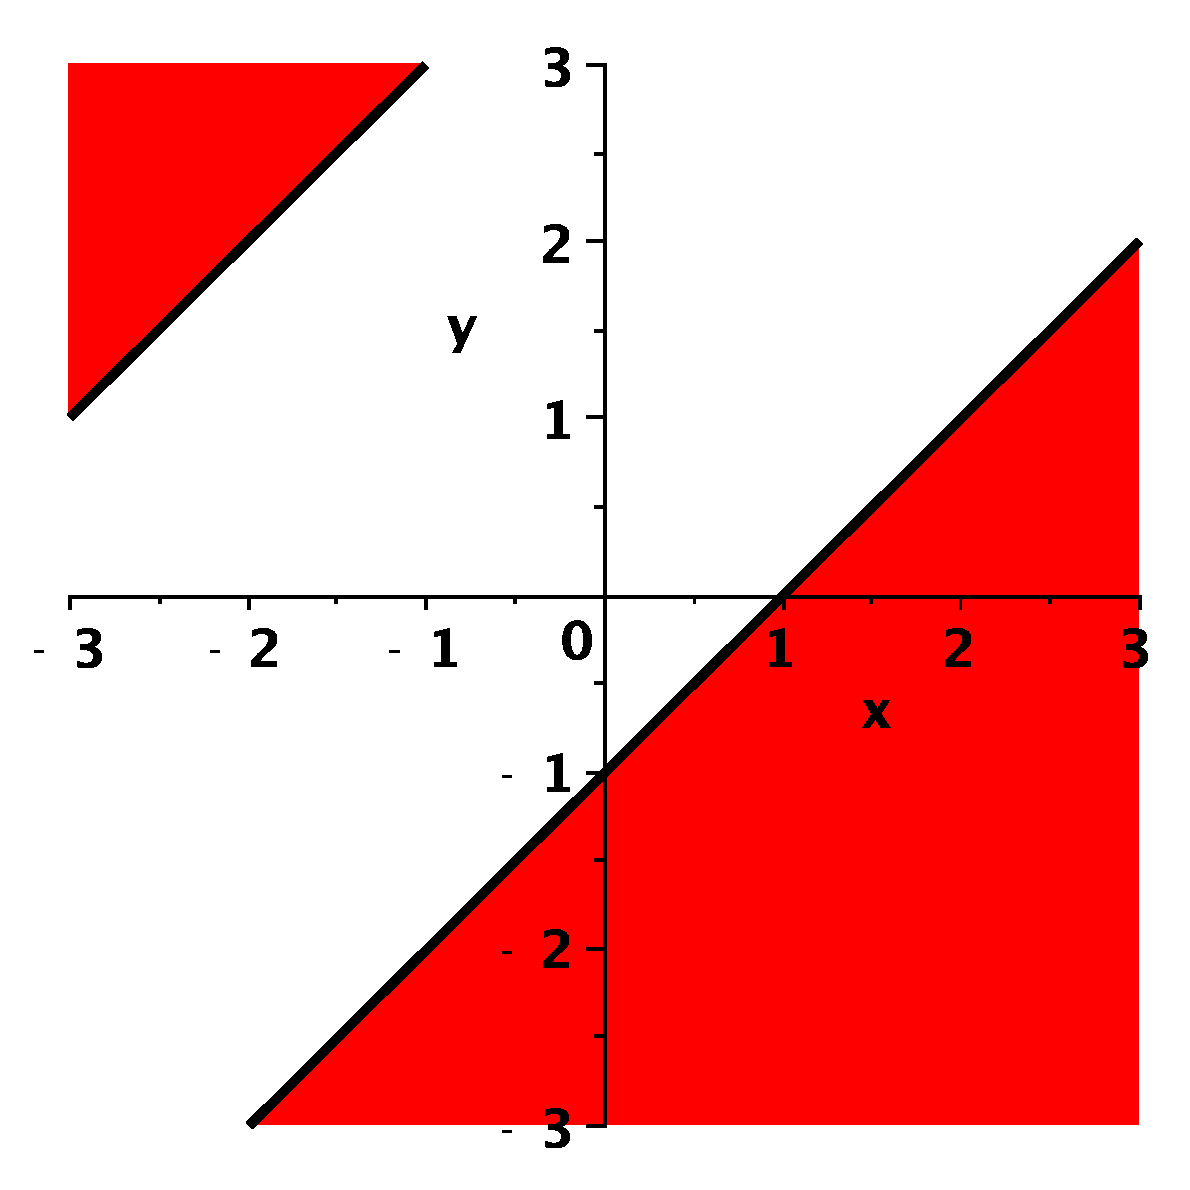
\includegraphics[width=8cm]{alg91.eps}
% alg91.eps : 300dpi, width=3.39cm, height=3.39cm, bb=0 0 400 400
\end{center}
Therefore, the answer is : false.\\

4092-- George is a farmer. He has at least two times less calves
than cows. There is room in his farm for no more than 15 calves and
40 cows. What graphic described the situation?\\

\begin{tabular}{l l}
a$)$ & b$)$\\
\includegraphics[width=8cm]{alg77.eps}
% alg77.eps : 300dpi, width=3.39cm, height=3.39cm, bb=0 0 400 400
& 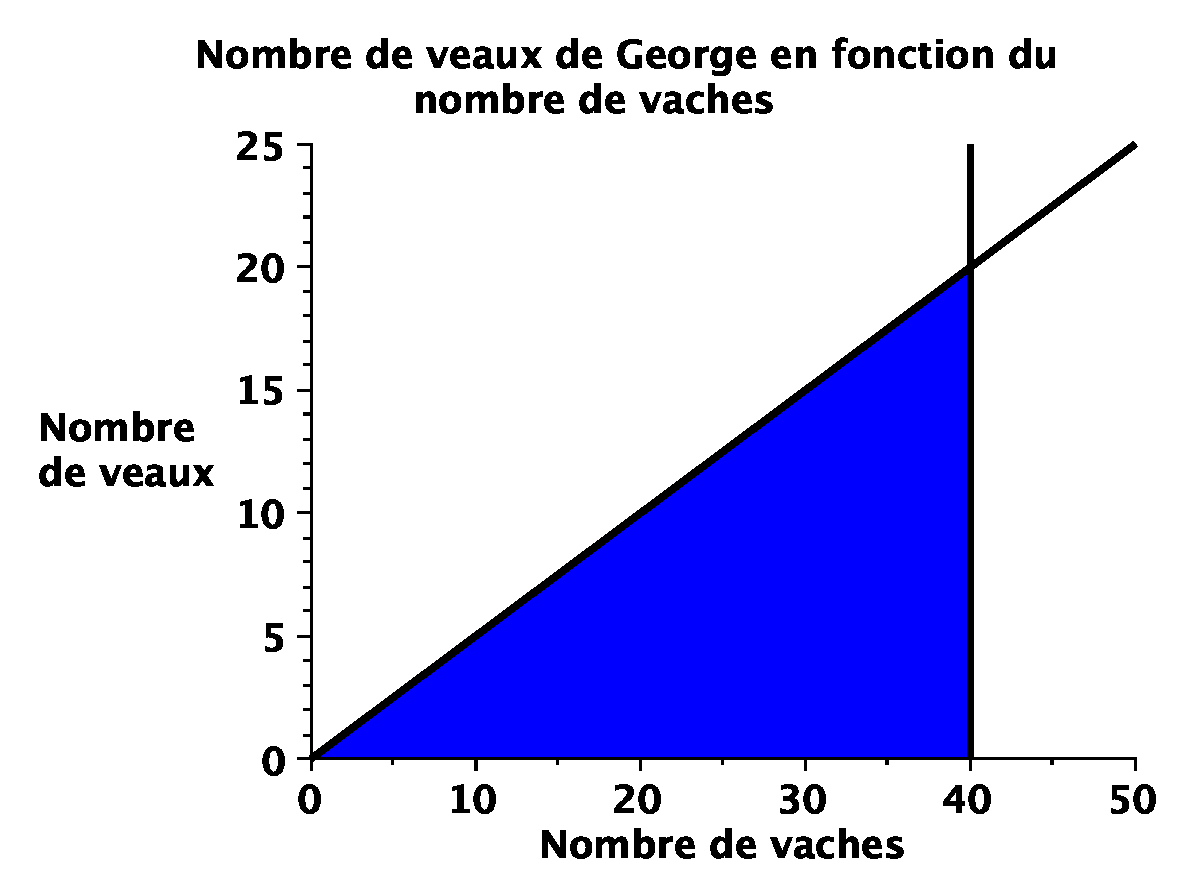
\includegraphics[width=9cm]{alg92.2.eps}\\
% alg92.2.eps : 300dpi, width=3.39cm, height=3.39cm, bb=0 0 400 400
c$)$ & d$)$\\
\includegraphics[width=9cm]{alg92.3.eps}
% alg92.3.eps : 300dpi, width=3.39cm, height=3.39cm, bb=0 0 400 400
& \includegraphics[width=9.5cm]{alg92.4.eps}\\
% alg92.4.eps : 300dpi, width=3.39cm, height=3.39cm, bb=0 0 400 400
\end{tabular}

R\'eponse : c$)$\\

R\'etroaction :\\

We are looking for the graphic that represents the following situation:\\
George is a farmer. He has at least two times less calves than cows.
There is room in his farm for no more than 15 calves and
40 cows.\\

Lets first identify the inequalities inherent to the situation. Let
$x$ be the number of cows and $y$ the number of calves. We then
have:
\begin{center}
$y \leq \frac{x}{2}$\\
$y\leq 15$\\
$x\leq 40$
\end{center}
So the right graphic is the one containing the three straight lines:
\begin{center}
$y = \frac{x}{2}$\\
$y = 15$\\
$x = 40$
\end{center}
We have to choose between the third and fourth graphic. We want
$y\leq 15$, so the right one is:
\begin{center}
\includegraphics[width=9cm]{alg92.3.eps}
% alg92.3.eps : 300dpi, width=3.39cm, height=3.39cm, bb=0 0 400 400
\end{center}
Therefore, the answer is c$)$.\\


4095-- Here's a system of inequalities:
\begin{center}
$y \geq 4+x$\\
$y > \frac{x}{3}+3$
\end{center}
What graphic represents the solution of the system?
\begin{center}
\begin{tabular}{l l}
a$)$ & b$)$\\
\includegraphics[width=7cm]{alg95.1.eps}
% alg95.1.eps : 300dpi, width=3.39cm, height=3.39cm, bb=0 0 400 400
& \includegraphics[width=7cm]{alg95.2.eps}\\
% alg95.2.eps : 300dpi, width=3.39cm, height=3.39cm, bb=0 0 400 400
c$)$ & d$)$\\
\includegraphics[width=7cm]{alg95.3.eps}
% alg95.3.eps : 300dpi, width=3.39cm, height=3.39cm, bb=0 0 400 400
& \includegraphics[width=7cm]{alg95.4.eps}\\
% alg95.4.eps : 300dpi, width=3.39cm, height=3.39cm, bb=0 0 400 400
\end{tabular}
\end{center}
R\'eponse : a$)$\\

R\'etroaction :\\

We are looking for the solution of:
\begin{center}
$y \geq 4+x$\\
$y > \frac{x}{3}+3$
\end{center}

Because $y \geq 4+x$, the solution is above the straight line $y =
4+x$ and the line is full because it is part of the solution.
Moreover, the solution is above the line $y =\frac{x}{3}+3$ and the
line is dotted because $y
> \frac{x}{3}+3$. So the graphic is:
\begin{center}
\includegraphics[width=7cm]{alg95.1.eps}
% alg95.1.eps : 300dpi, width=3.39cm, height=3.39cm, bb=0 0 400 400
\end{center}
Therefore, the answer is a$)$.\\


4097-- Here's a system of inequalities:
\begin{center}
$y \geq 4-x$\\
$y > 4+2x$
\end{center}
What letter on the graphic represents the solution of the system?
\begin{center}
\includegraphics[width=7cm]{alg94.eps}
% alg94.eps : 300dpi, width=3.39cm, height=3.39cm, bb=0 0 400 400
\end{center}

a$)$ A\\
b$)$ B\\
c$)$ C\\
d$)$ D\\

R\'eponse : b$)$\\

R\'etroaction :\\

We are looking for the solution of:
\begin{center}
$y \geq 4-x$\\
$y > 4+2x$
\end{center}
in this graphic:
\begin{center}
\includegraphics[width=7cm]{alg94.eps}
% alg94.eps : 300dpi, width=3.39cm, height=3.39cm, bb=0 0 400 400
\end{center}
Because $y \geq 4-x$, the solution is above the straight line $y =
4-x$ and the solution is either B or C. Moreover, the solution is
above $y = 4+2x$ because $y > 4+2x$. So the solution is found in B.\\
Therefore, the answer is b$)$.\\


4101-- Eve works in a convenience store. She wishes to get the best
income as possible from selling slush. She knows that she can't
produce more than 22 liters of ice a day. Moreover, she has no more
than 30 glasses of 250ml and 40 of 500ml. She sells a small slush
$2,00\,\$$ and a tall one $3,50\,\$$.
\begin{center}
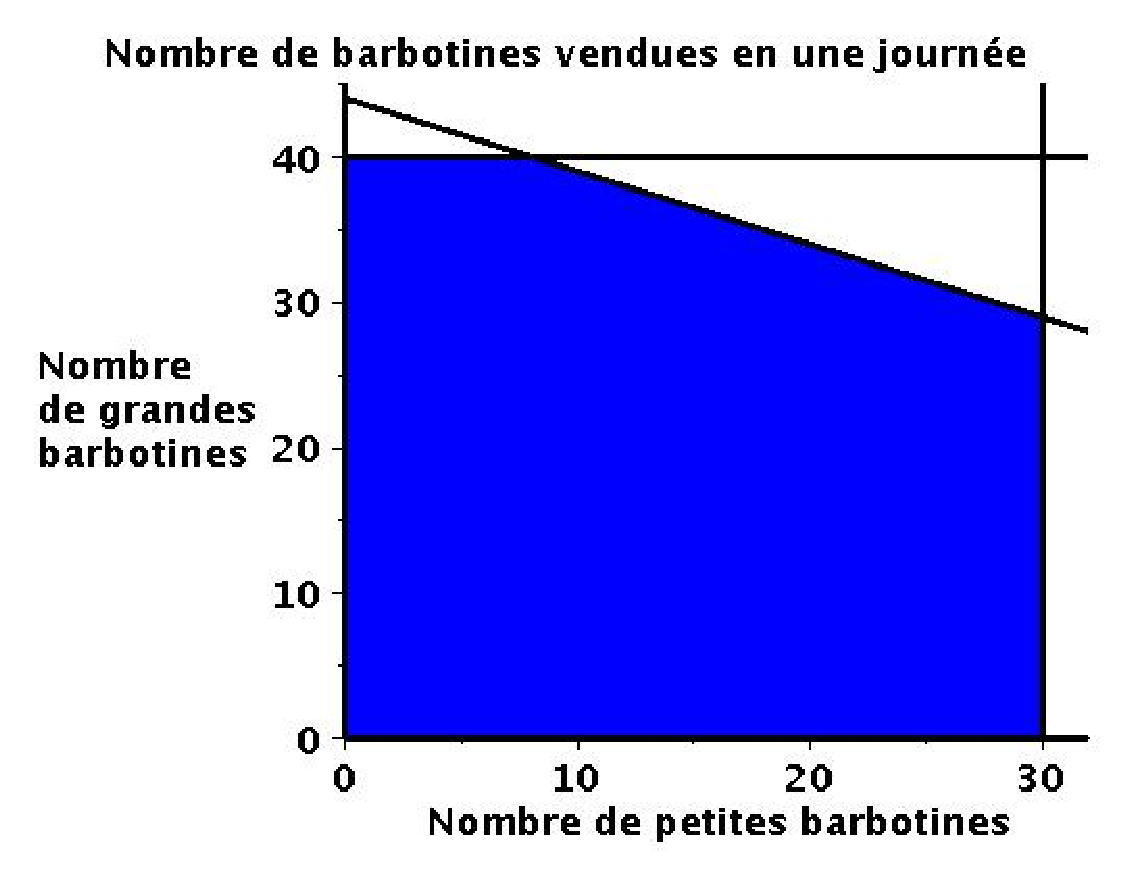
\includegraphics[width=9cm]{alg100.eps}
% alg100.eps : 300dpi, width=3.39cm, height=3.39cm, bb=0 0 400 400
\end{center}
What point is not an vertex in the restriction polygon?\\

a$)$ $\left(0,\,0\right)$\\
b$)$ $\left(0,\,40\right)$\\
c$)$ $\left(8,\,40\right)$\\
d$)$ $\left(30,\,30\right)$\\


R\'eponse : d$)$\\

R\'etroaction:\\

We are looking for the point that is not an vertex in the
restriction polygon.
\begin{center}
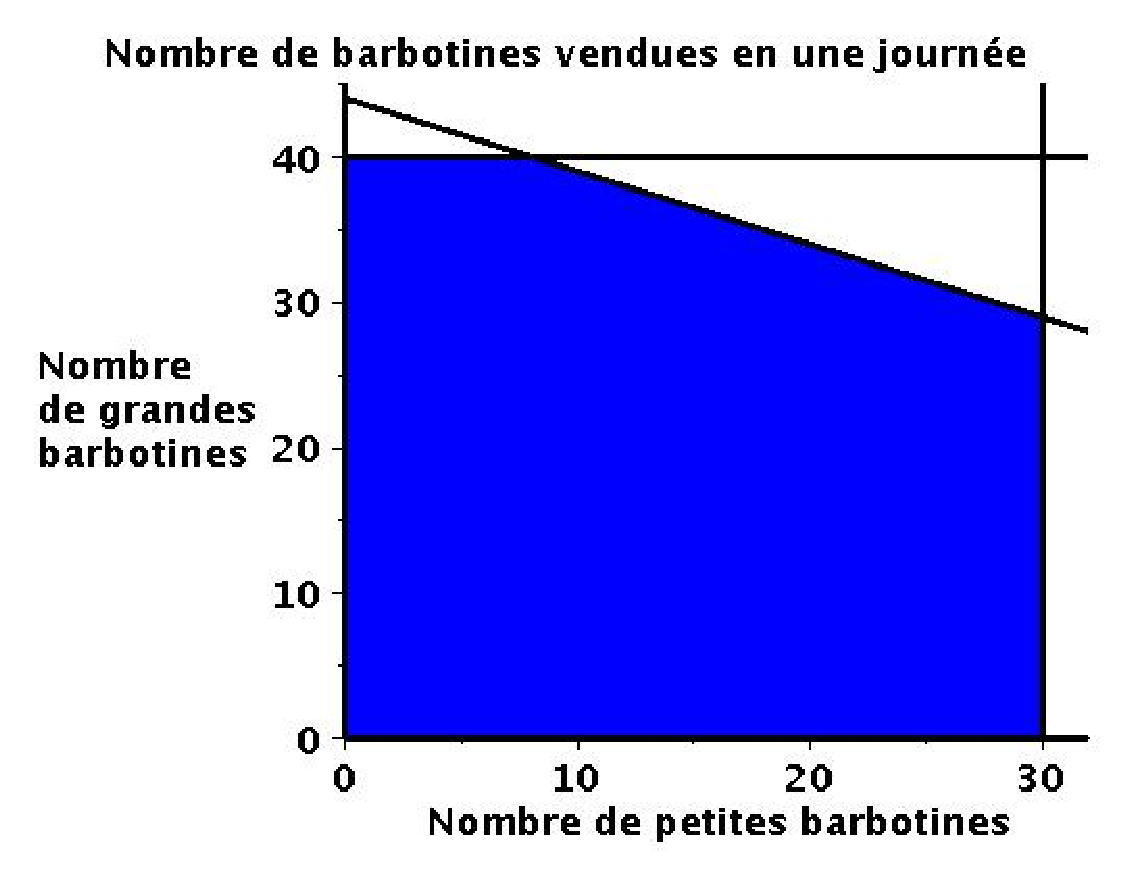
\includegraphics[width=9cm]{alg100.eps}
% alg100.eps : 300dpi, width=3.39cm, height=3.39cm, bb=0 0 400 400
\end{center}
The points $\left(0,\,0\right)$, $\left(0,\,40\right)$ and
$\left(8,\,40\right)$ are vertexes while $\left(30,\,30\right)$ is
not. We have to find the intersection between the straight line:
\begin{eqnarray*}
p=30\\
0,250p+0,500g=22
\end{eqnarray*}
The intersection is at $\left(30,\,g_1\right)$. We find $g_1$ with:
\begin{eqnarray*}
0,250p+0,500g_1 &=& 22\\
0,250\times30+0,500g_1&=&22\\
7,5+0,500g_1&=&22\\
0,500g_1&=&14,5\\
g_1&=&29
\end{eqnarray*}
So the vertex is at $\left(30,\,29\right)$ and not at
$\left(30,\,30\right)$.\\
Therefore, the answer is d$)$.\\


4116-- Jeremy starts working this summer by harvesting fruits. He
wants to maximize his daily earnings. In July, he's picking
strawberries and raspberries. He picks a basket of strawberries in
45 minutes and gets 5 \$ from it while a basket of raspberries takes
him an hour to pick and gets him 8 \$. His boss wants him to pick
strawberries for at least 3 hours and 45 minutes a day. He has to
pick at least 8 baskets a day but no more than 10.\\
If he gets the most money out of his job, what is his average hourly
salary rounded to the hundredth.\\

a$)$ 2,25 \$/h\\
b$)$ 4,50 \$/h\\
c$)$ 7,19 \$/h\\
d$)$ 7,43 \$/h\\

R\'eponse : d$)$\\

R\'etroaction:\\

We are looking for Jeremy's hourly salary on a day he gets the
maximum daily earnings.\\
We first have to know how many baskets of each strawberries and
raspberries he's picking on a top earning day. Then the profit made
from those baskets has to be divided by the time needed to pick them
up.\\

So here's the situation:\\
He picks a basket of strawberries in 45 minutes and gets 5 \$ from
it while raspberries takes him an hour and is worth 8 \$. His boss
wants him to pick strawberries for at least 3 hours and 45 minutes a
day. He has to pick at least 8 baskets a day but no more than 10.\\

Let $x$ be the number of baskets of strawberries and $y$ the number
of baskets of raspberries. Here are the restrictions:
\begin{eqnarray*}
x\geq5\\
x+y\geq8\\
x+y\leq10
\end{eqnarray*}

The restriction polygon is then:
\begin{center}
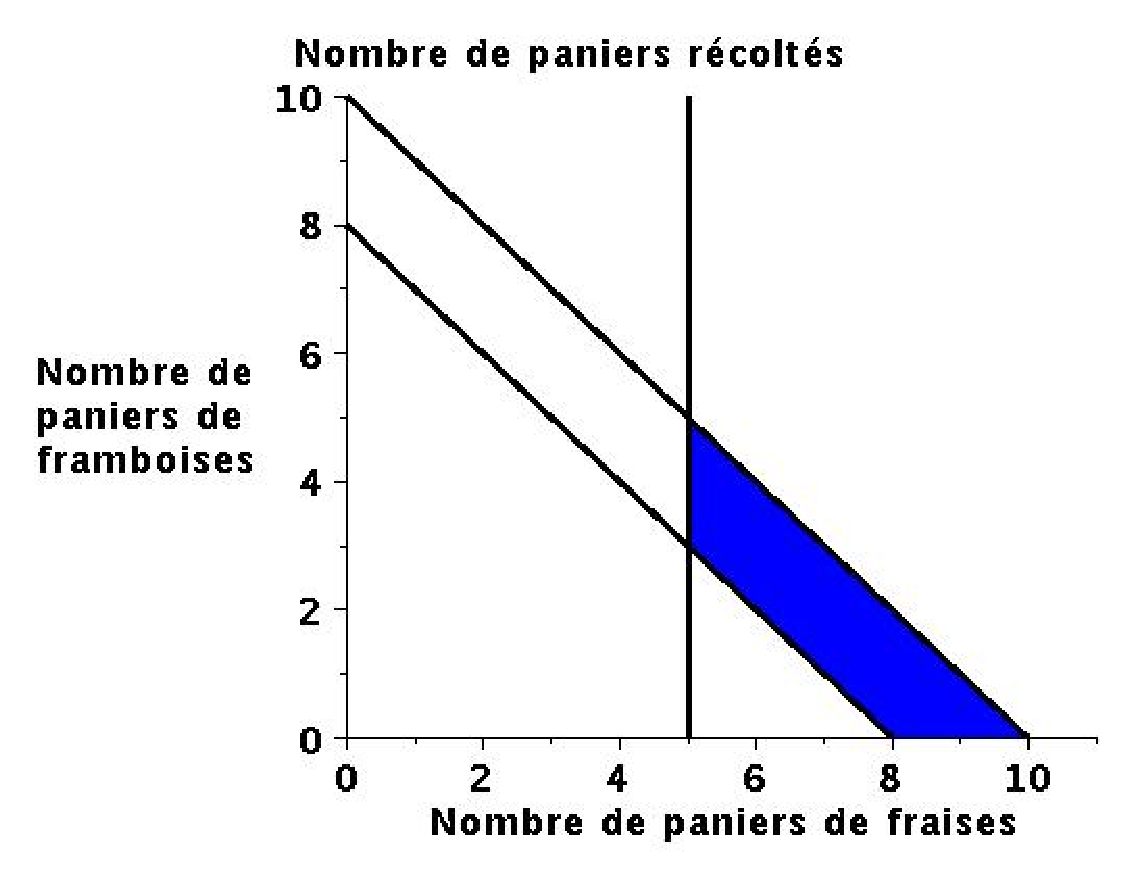
\includegraphics[width=9cm]{alg105.1.eps}
% alg105.1.eps : 300dpi, width=3.39cm, height=3.39cm, bb=0 0 400 400
\end{center}

The polygon vertexes are: $\left(5,\,3\right)$,
$\left(5,\,5\right)$, $\left(8,\,0\right)$ and $\left(10,\,0\right)$.\\

The function to be maximized is $S=5x+8y$ since strawberries baskets
are 5 \$ and raspberries baskets are 8 \$.\\

The earnings are evaluated for each vertex:\\
$\left(5,\,3\right)$ $\Longleftrightarrow$ $S=5\times5+8\times3=25+24=49$\\
$\left(5,\,5\right)$ $\Longleftrightarrow$ $S=5\times5+8\times5=25+40=65$\\
$\left(8,\,0\right)$ $\Longleftrightarrow$ $S=5\times8+8\times0=40+0=40$\\
$\left(10,\,0\right)$ $\Longleftrightarrow$ $S=5\times10+8\times0=50+0=50$\\

So the top salary is 65 \$ and is reached when Jeremy picks 5
baskets of strawberries and 5 baskets of raspberries. The time
needed to pick them is: $T=5\times0,75$ hour $+5\times1$ hour
$=3,75$ hours $+5$
hours$=8,75$ hours.\\

So Jeremy gets 65 \$ in 8,75 hours. He's then payed 7,43 \$/h.\\
Therefore, the answer is d$)$.\\

4128-- Here are some inequalities:
\begin{eqnarray*}
3x^2+|z|-2y&\geq&5-5x\\
3x^2-5+5x&\geq&2y+Jx^2-|z|
\end{eqnarray*}

True or false?\\
If the constant $J$ takes the value 0 the inequalities are not
equivalent.\\

R\'eponse : False\\

R\'etroaction:\\

The question is to know wether the inequalities are equivalent when
$J$ is worth 0.
\begin{eqnarray*}
3x^2+|z|-2y&\geq&5-5x\\
3x^2-5+5x&\geq&2y+Jx^2-|z|
\end{eqnarray*}
Lets put that value in the inequality and transform it in order to
compare it with the other one:
\begin{eqnarray*}
3x^2-5+5x&\geq&2y+0x^2-|z|\\
3x^2-5+5x&\geq&2y-|z|\\
3x^2-5+5x-2y&\geq&-|z|\\
3x^2-5+5x+|z|-2y&\geq&0\\
3x^2+5x+|z|-2y&\geq&5\\
3x^2+|z|-2y&\geq&5-5x
\end{eqnarray*}
So the two inequalities are equivalent when $J=0$. According to the
question, if the constant $J$ takes the value 0 the inequalities are
not equivalent, the answer is false.\\
Therefore, the answer is : false.\\

4129-- Which of the following inequalities is or are equivalent to
this one?
\begin{eqnarray*}
6x-2y\geq\frac{15-5x}{10}
\end{eqnarray*}

1$)$ $-20y\geq15-55x $\\[2mm]
2$)$ $ -y\geq \frac{15-65x}{20}$\\[2mm]
3$)$ $ y\geq \frac{15-55x}{20}$\\[2mm]
4$)$ $ y\leq \frac{65x-15}{20}$\\[2mm]

a$)$ 1 and 2\\
b$)$ 2 and 4 \\
c$)$ 3 and 4\\
d$)$ 4 \\

R\'eponse : b$)$\\

R\'etroaction:\\

We are looking for the one or ones between:\\

1$)$ $-20y\geq15-55x $\\[2mm]
2$)$ $ -y\geq \frac{15-65x}{20}$\\[2mm]
3$)$ $ y\geq \frac{15-55x}{20}$\\[2mm]
4$)$ $ y\leq \frac{65x-15}{20}$\\[2mm]

equivalent to:
\begin{eqnarray*}
6x-2y\geq\frac{15-5x}{10}
\end{eqnarray*}
We have to modify it to find the equivalence or equivalences.
\begin{eqnarray*}
6x-2y&\geq&\frac{15-5x}{10}\\
60x-20y&\geq&15-5x\\
-20y&\geq&15-65x\\
-y&\geq&\frac{15-65x}{20}\\
y&\leq&\frac{-\left(15-65x\right)}{20}\\
y&\leq&\frac{65x-15}{20}
\end{eqnarray*}
According to the third line of the transformation the first choice
is not equivalent. With the fourth line, we see that the second
choice is right. The last line shows that the third choice is not
equivalent and that the fourth is. So the equivalent inequalities are 2 and 4.\\
Therefore, the answer is b$)$.\\

4130-- Which of the following inequalities is or are equivalent to
this one?
\begin{eqnarray*}
6x^2-2y\geq\frac{15x-5x^3+60x^2}{5x}+4y
\end{eqnarray*}

1$)$ $-6y\geq3-5x^2+60x$\\[2mm]
2$)$ $ -y\geq\frac{3-7x^2+12x}{6}$\\[2mm]
3$)$ $ y\geq\frac{7x^2-12x-3}{6}$\\[2mm]
4$)$ $ y\leq\frac{7x^2-12x-3}{2}$\\[2mm]

a$)$ 1 and 2\\
b$)$ 2 \\
c$)$ 2 and 4\\
d$)$ 3 \\

R\'eponse : b$)$\\

R\'etroaction:\\

We are looking for the one or ones between:\\

1$)$ $-6y\geq3-5x^2+60x$\\[2mm]
2$)$ $ -y\geq\frac{3-7x^2+12x}{6}$\\[2mm]
3$)$ $ y\geq\frac{7x^2-12x-3}{6}$\\[2mm]
4$)$ $ y\leq\frac{7x^2-12x-3}{2}$\\[2mm]

equivalent to:
\begin{eqnarray*}
6x^2-2y\geq\frac{15x-5x^3+60x^2}{5x}+4y
\end{eqnarray*}
We have to modify it to find the equivalence or equivalences.
\begin{eqnarray*}
6x^2-2y&\geq&\frac{15x-5x^3+60x^2}{5x}+4y\\
6x^2-6y&\geq&\frac{15x-5x^3+60x^2}{5x}\\
6x^2-6y&\geq&3-x^2+12x\\
-6y&\geq&3-7x^2+12x\\
-y&\geq&\frac{3-7x^2+12x}{6}\\
y&\leq&\frac{-\left(3-7x^2+12x\right)}{6}\\
y&\leq&\frac{7x^2-12x-3}{6}
\end{eqnarray*}
According to the fourth line of the transformation the first choice
is not equivalent. With the fifth line, we see that the second
choice is right. The last line shows that the third and fourth
choices are not equivalent. So the equivalent inequality is 2.\\
Therefore, the answer is b$)$.\\

4131-- Which inequality is totally included in this one?
\begin{eqnarray*}
3+y\geq4x
\end{eqnarray*}

a$)$ $ y\leq4x$\\[2mm]
b$)$ $ 3+y\leq4x$\\[2mm]
c$)$ $ 5+y\geq4x$\\[2mm]
d$)$ $ y\geq4x$\\[2mm]

R\'eponse : d$)$\\

R\'etroaction:\\

We are looking for the inequality among $y\leq4x$, $3+y\leq4x$,
$5+y\geq4x$ and $y\geq4x$ that is totally included in $3+y\geq4x$.\\

All inequalities in this problem are restricted by parallel straight
lines since they all have the same slope which is 4. The inequality
$3+y\geq4x$ is represented by a straight line in black, which y-axis
intersect is at -3, and the space above that line (in yellow and
green) because $y$ is greater than the expression. There has to be
an other inequality which y-axis intersect is greater than -3 and
for which $y$ is greater than the expression. The one that is within
the restrictions is $y\geq4x$. The blue line that bounds the green
region has a y-axis intersect of 0 and $y$ is greater than the
expression.
\begin{center}
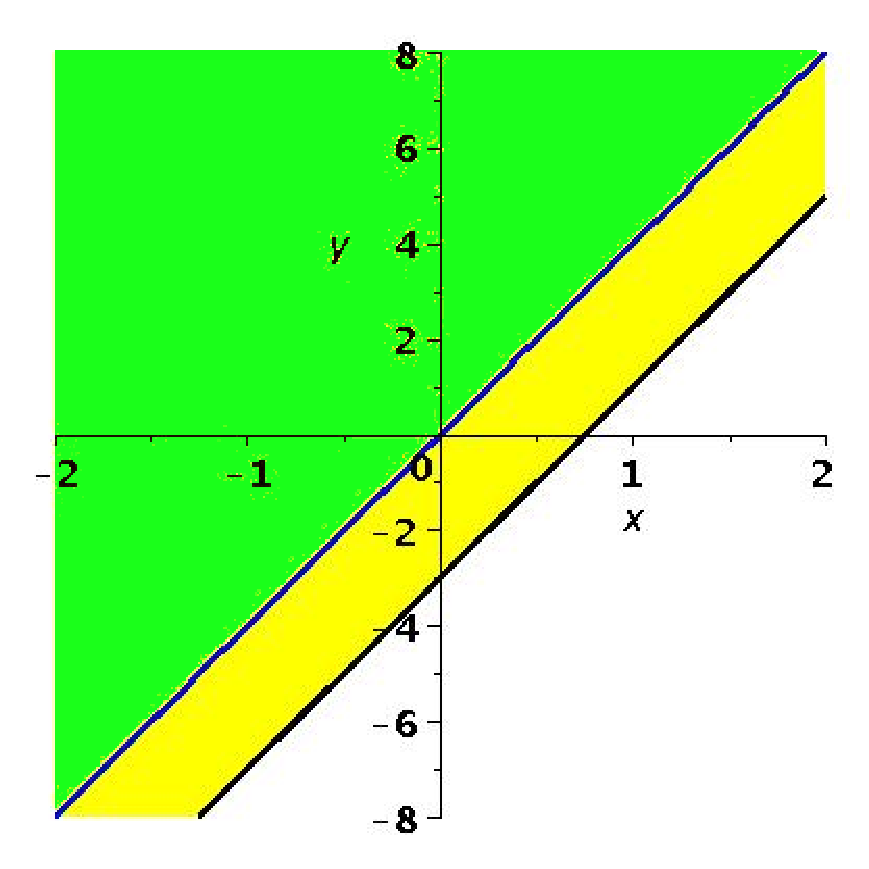
\includegraphics[width=8cm]{alg131.eps}
% alg105.1.eps : 300dpi, width=3.39cm, height=3.39cm, bb=0 0 400 400
\end{center}
Therefore, the answer is d$)$.\\

4132-- Which inequality is totally included in this one?
\begin{eqnarray*}
\frac{3-y}{5}\geq x
\end{eqnarray*}

a$)$ $ -5+y\leq-5x$\\[2mm]
b$)$ $ 3+y\leq5x$\\[2mm]
c$)$ $ 5+y\leq-5x$\\[2mm]
d$)$ $ y\geq-5x$\\[2mm]

R\'eponse : c$)$\\

R\'etroaction:\\

We are looking for the inequality among $-5+y\leq-5x$, $3+y\leq5x$,
$5+y\leq-5x$ and $y\geq-5x$, that is totally included in $\frac{3-y}{5}\geq x$.\\

For an inequality to be totally included in an other one, both
straight lines bounding those inequalities have to be parallel. The
answer is then an inequality which slope is the same as the one for
$\frac{3-y}{5}\geq x$. The slope is found like this:
\begin{eqnarray*}
\frac{3-y}{5}&\geq& x\\
3-y&\geq& 5x\\
-y&\geq& 5x-3\\
y&\leq& 3-5x
\end{eqnarray*}
So the line's slope bounding the equation is -5. Among the choices,
the inequations 1, 3 and 4 have slopes of -5.\\
Moreover, the inequality $y\leq 3-5x$ is represented by a black
line, which y-axis intersect is at 3 and the space in yellow and
green below that line, because $y$ is smaller than the expression.
Among 1, 3 and 4, we have to find the one for which the y-axis
intersect is smaller than 3 so $y$ is smaller than the expression.
The inequality $5+y\leq-5x$ is fulfills the conditions with the blue
line bounding the green region, its y-axis intersect at -5 and $y$
is smaller than the expression.
\begin{center}
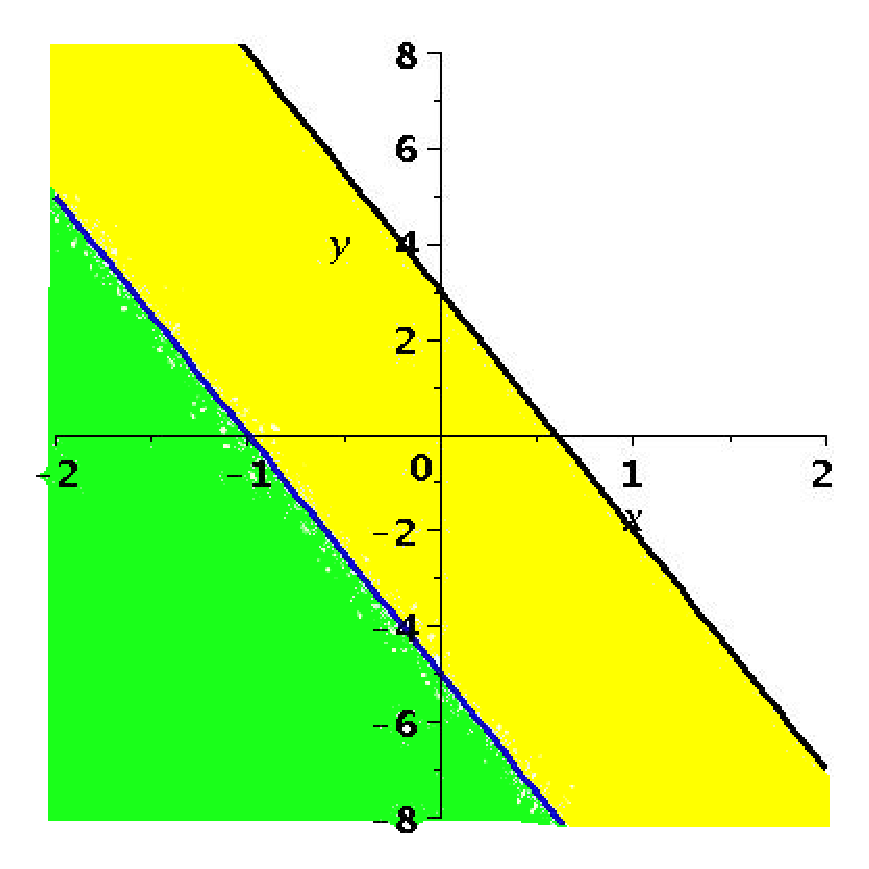
\includegraphics[width=8cm]{alg132.eps}
% alg105.1.eps : 300dpi, width=3.39cm, height=3.39cm, bb=0 0 400 400
\end{center}
Therefore, the answer is c$)$.\\

4133-- Frank works in a shoe store. He's payed 8 \$ an hour. What is
the initial value of the relation associated to that situation?\\

R\'eponse : 0\\

R\'etroaction :\\

We are looking for the initial value of the situation represented by
Frank working in a shoe store and payed 8 \$ an hour.\\

The independent variable of the situation is the number of hours of
work and the dependent one is the salary. The rate of change is 8 \$
and because he's salary is null if he doesn't work, the initial
value is 0.\\
Therefore, the answer is 0.\\


4139-- What am I?\\
I am the value of the dependent variable of a relation when the
independent variable is null.\\

a$)$ The final value\\
b$)$ The zero\\
c$)$ The rate of change\\
d$)$ The y-axis intersect\\

R\'eponse : d$)$\\

R\'etroaction :\\

The value of the dependent variable of a relation when the
independent variable is null is the y-axis intersect.\\
Therefore, the answer is d$)$.\\

4140-- What am I?\\
I am the variation of the variable $y$ when the variable $x$
raises by 1.\\

a$)$ The final value\\
b$)$ The zero\\
c$)$ The rate of change\\
d$)$ The y-axis intersect\\

R\'eponse : c$)$\\

R\'etroaction :\\

The variation of the variable $y$ when the variable
$x$ raises by 1 is the rate of change of the relation, or the slope.\\
Therefore, the answer is c$)$.\\

4141-- Five weeks ago, Catherine decided to save some money. She had
345\$ in the beginning and she now has
420\$. How much money is she saving each week?\\

R\'eponse : 15 \$\\

R\'etroaction:\\

We are looking for the amount of money saved by Catherine each week.
We know that she had 345 \$ five weeks ago and now has 420 \$.\\

So in five weeks she saved 420 - 345 = 75 \$. Each week she saved:
$75\$\div5$ weeks $= 15\,\$$ a week. The weekly savings are then 15 \$.\\
Therefore, the answer is 15 \$.\\

4142-- George is emptying his pool with a pump that has an unknown
flow rate. He wants you to calculate the flow rate to know the time
needed to empty the pool. There is 13 m$^3$ of water before starting
to empty. After 30 minutes, there is 10 m$^3$ remaining.\\

The flow rate of the pump is:

a$)$ $-3$ m$^3$ per 30 minutes\\
b$)$ $1$ m$^3$ per 10 minutes\\
c$)$ $3$ m$^3$ per hour\\
d$)$ $9$ m$^3$ per hour\\

R\'eponse : b$)$\\

R\'etroaction:\\

We are looking the flow rate of the pump knowing:
\begin{itemize}
\item there is 13 m$^3$ of water in the pool before starting emptying it.
\item after 30 minutes, there is 10 m$^3$ remaining.
\end{itemize}
In 30 minutes, $13-10=3$ m$^3$ of water went trough the pump. The
flow rate is found with: $3$ m$^3\div0,5$ hour $=$ 6 m$^3$ per hour.
So the answer can't be neither c$)$ nor d$)$. The flow rate of the
pump is strictly positive. Thus, a$)$ can't the answer. The b$)$
answer, $1$ m$^3$ per 10 minutes, is equivalent to $6$ m$^3$ per
hour because six times less liquid flow in six times less time.\\
Therefore, the answer is b$)$.\\

4143-- What is the rate od change of the following relation?
\begin{center}
 \includegraphics[width=8cm]{fonction136.eps}
 % fonction1.eps: 1048592x1048592 pixel, 0dpi\begin{center}
\end{center}

a$)$ $-6$\\
b$)$ $-3$\\
c$)$ $-2$\\
d$)$ 3\\

R\'eponse : b$)$\\

R\'etroaction :\\

We are looking for the rate of change of the situation:
\begin{center}
 \includegraphics[width=8cm]{fonction136.eps}
 % fonction1.eps: 1048592x1048592 pixel, 0dpi\begin{center}
\end{center}
The rate of change is the variation of the variable $y$ when the
variable $x$ raises by 1. On the graphic, as $x$ goes from $-2$ to
$-1$, $y$ goes from 0 to $-3$. The value of $y$ has lowered by 3 so
the rate of change is $-3$.\\
Therefore, the answer is b$)$.\\


4152-- The following graphic links a cone's volume with its radius.
The height of the cone is fixed.
\begin{center}
 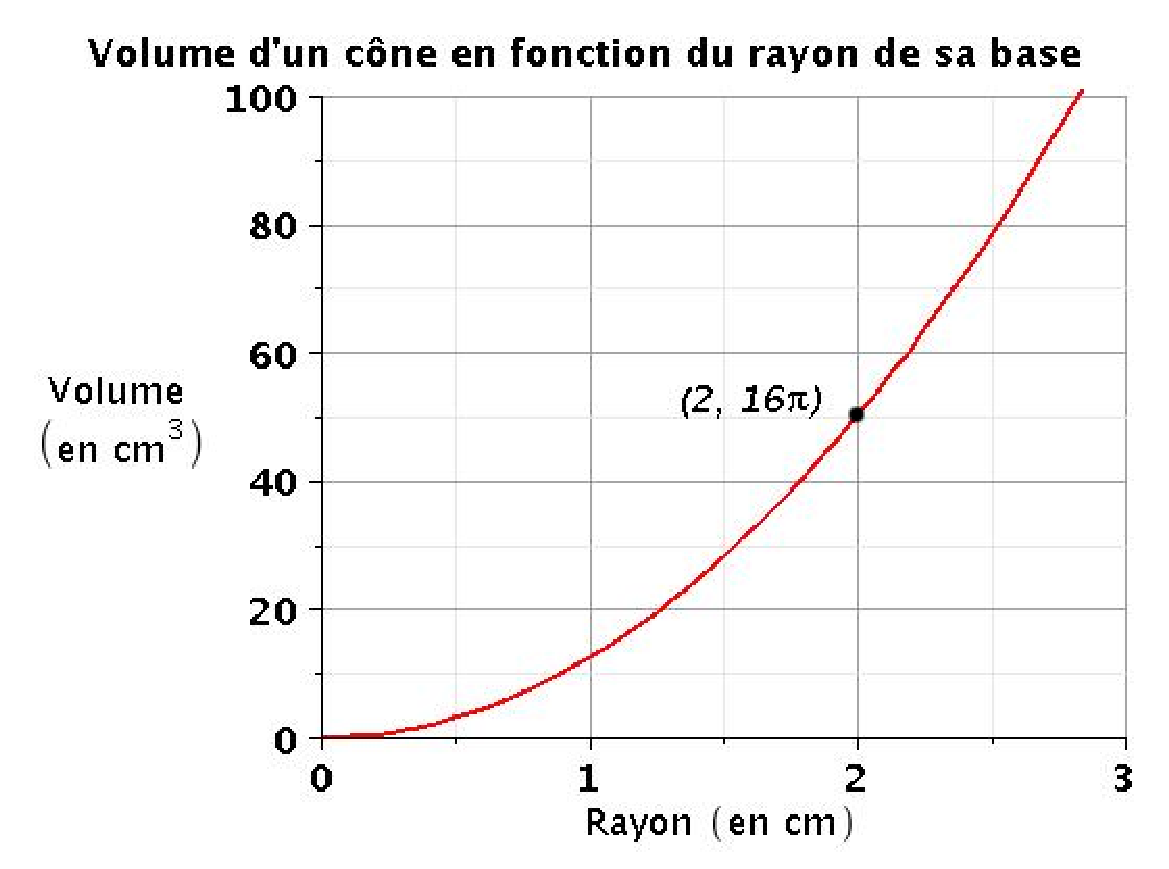
\includegraphics[width=9cm]{fonction152.eps}
 % fonction1.eps: 1048592x1048592 pixel, 0dpi\begin{center}
\end{center}
What is the rule of the relation?\\

a$)$ $v=\pi r^4$\\
b$)$ $v=2\pi r^3$\\
c$)$ $v=4\pi\sqrt r$\\
d$)$ $v=4\pi r^2$\\

R\'eponse : d$)$\\

R\'etroaction:\\

We are looking for the rule of the relation:
\begin{center}
 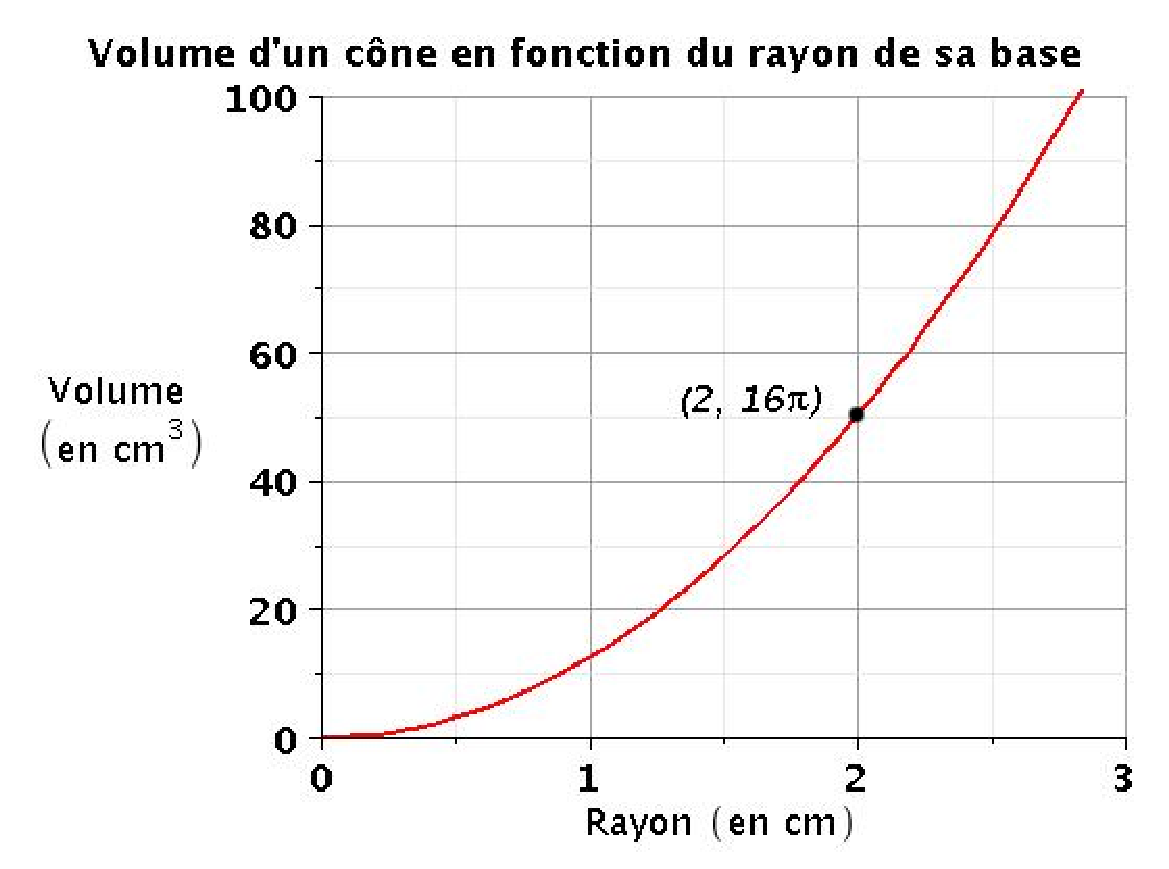
\includegraphics[width=9cm]{fonction152.eps}
 % fonction1.eps: 1048592x1048592 pixel, 0dpi\begin{center}
\end{center}
Let $r$ be the radius of the base of the cone and $v$ its volume.
The volume equation of a cone is:
\begin{eqnarray*}
v&=&\frac{A_\textnormal{base}\times \textnormal{height}}{3}\\
&=&\frac{\pi r^2\times h}{3}\\
&=&\frac{\pi h r^2}{3}\\
&=&\frac{\pi h}{3}\times r^2\\
&=&\frac{a} r^2 \qquad\textnormal{where }a=\frac{\pi h}{3}
\end{eqnarray*}

Because the point $\left(2,\,16\pi\right)$ is part of the curve, we
can find the $a$ parameter by substitution in the rule.
\begin{eqnarray*}
v&=&ar^2\\
16\pi&=&a\times2^2\\
16\pi&=&a\times4\\
\frac{16\pi}{4}&=&a\\
4\pi&=&a
\end{eqnarray*}
The rule is: $v=4\pi r^2$.\\
Therefore, the answer is d$)$.\\

4153-- The following graphic links a cone's volume with its radius.
The height of the cone is fixed.
\begin{center}
 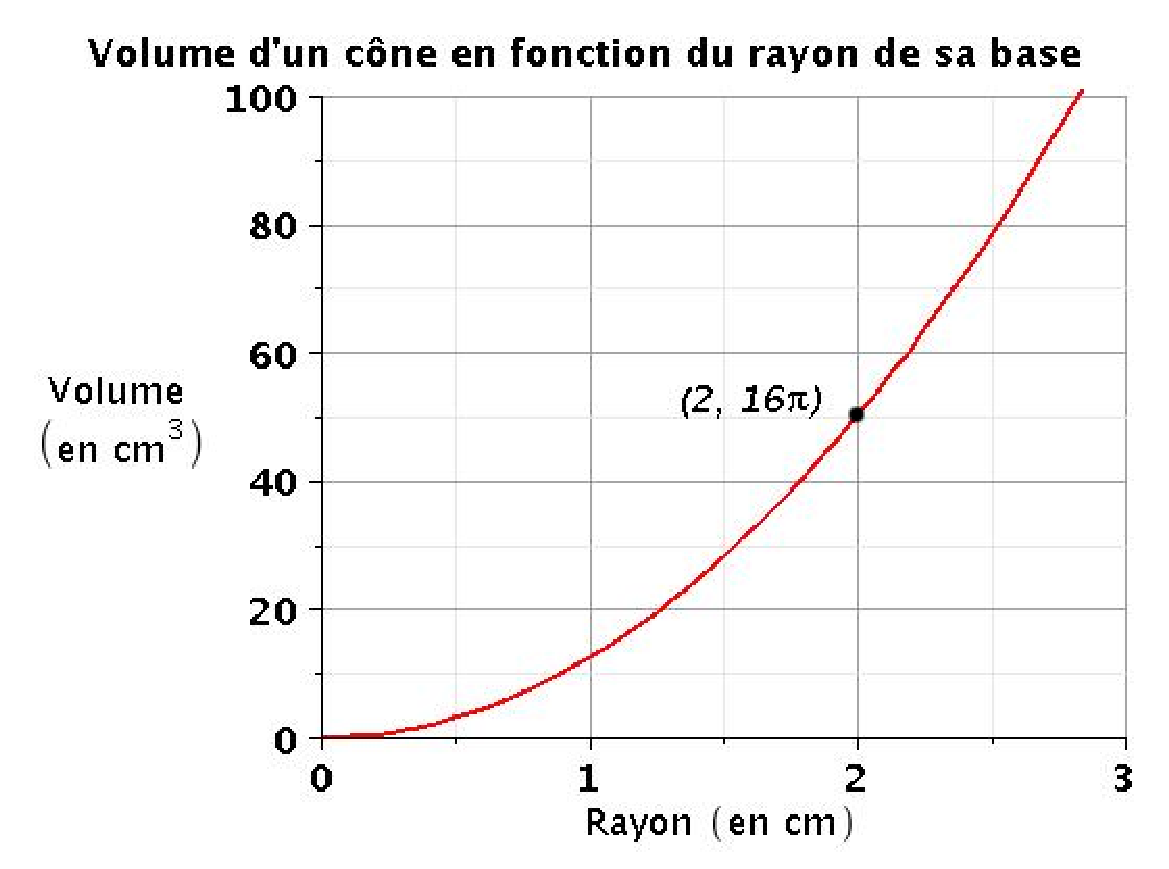
\includegraphics[width=9cm]{fonction152.eps}
 % fonction1.eps: 1048592x1048592 pixel, 0dpi\begin{center}
\end{center}
What is the height of the cone?\\

a$)$ 2 cm\\
b$)$ 4 cm\\
c$)$ 8 cm\\
d$)$ 12 cm\\

R\'eponse : d$)$\\

R\'etroaction:\\

We are looking for the height of the cone.
\begin{center}
 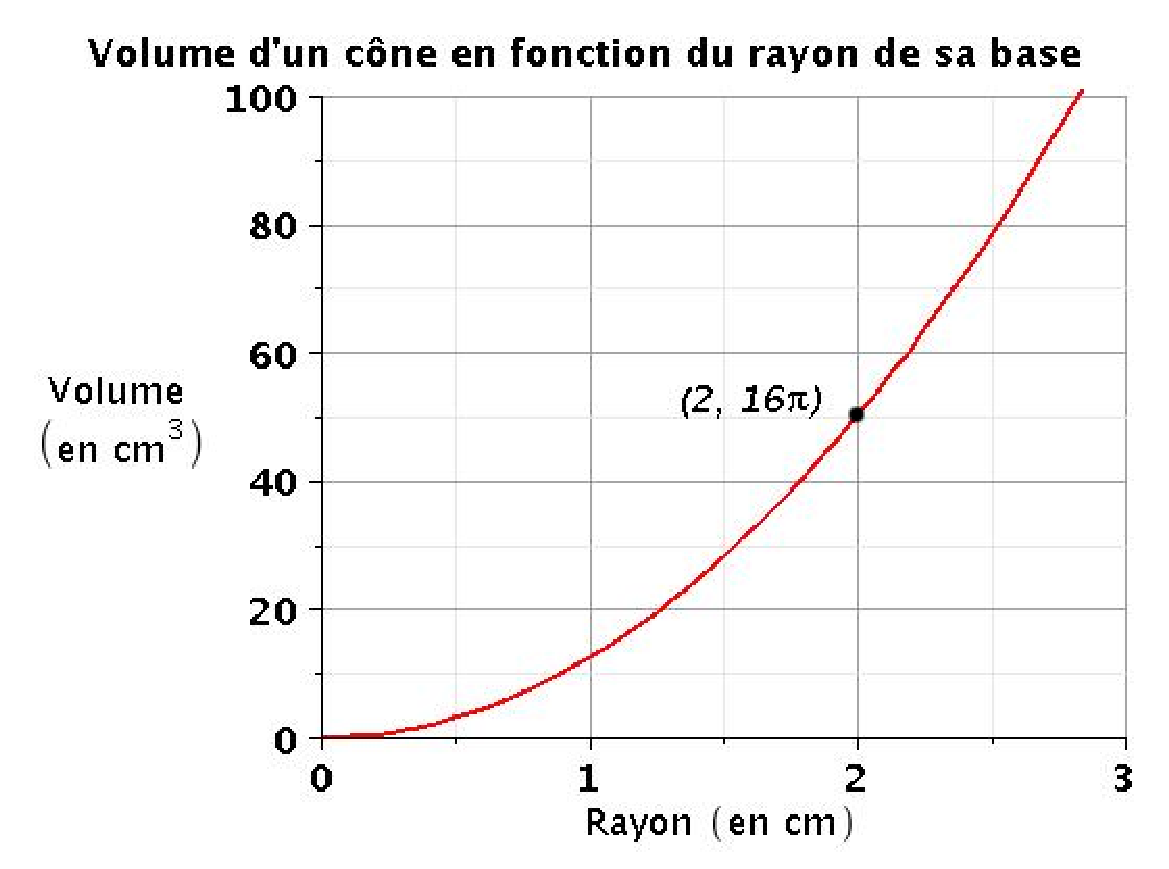
\includegraphics[width=9cm]{fonction152.eps}
 % fonction1.eps: 1048592x1048592 pixel, 0dpi\begin{center}
\end{center}
Let $r$ be the radius of the base of the cone and $v$ its volume.
The volume equation of a cone is:
\begin{eqnarray*}
v&=&\frac{A_\textnormal{base}\times \textnormal{height}}{3}\\
&=&\frac{\pi r^2h}{3}
\end{eqnarray*}
Because the point $\left(2,\,16\pi\right)$ is part of the curve, we
can find the $a$ parameter by substitution in the rule.
\begin{eqnarray*}
v&=&\frac{\pi r^2h}{3}\\
16\pi&=&\frac{\pi 2^2h}{3}\\
16\pi&=&\frac{4\pi h}{3}\\
4&=&\frac{h}{3}\\
12&=&h
\end{eqnarray*}
The height of the cone is then 12 cm.\\
Therefore, the answer is d$)$.\\

4154-- Which of the following equations is equivalent to $4y+5=x$?\\

a$)$ $4y=x+5$\\[2mm]
b$)$ $5=x+4y$\\[2mm]
c$)$ $y=\frac{x-5}{4}$\\[2mm]
d$)$ $y=\frac{x+5}{4}$\\[2mm]

R\'eponse: c$)$\\

R\'etroaction:\\

We are looking for an equation equivalent to $4y+5=x$.\\
Lets isolate $y$.
\begin{eqnarray*}
4y+5&=&x\\
4y&=&x-5\\
y&=&\frac{x-5}{4}
\end{eqnarray*}
Therefore, the answer is c$)$.\\

4155-- Which of the following equations is equivalent to $\frac{2}{5}y+5=2x$?\\

a$)$ $\frac{2}{5}y=2x+5$\\[2mm]
b$)$ $4y=x+5$\\[2mm]
c$)$ $y=\frac{4x}{5}-2$\\[2mm]
d$)$ $y=5x-\frac{25}{2}$\\[2mm]

R\'eponse: d$)$\\

R\'etroaction:\\

We are looking for an equation equivalent to $\frac{2}{5}y+5=2x$.\\
Lets isolate $y$.
\begin{eqnarray*}
\frac{2}{5}y+5&=&2x\\
\frac{2y}{5}&=&2x-5\\
2y&=&5\left(2x-5\right)\\
2y&=&10x-25\\
y&=&5x-\frac{25}{2}
\end{eqnarray*}
Therefore, the answer is d$)$.\\

4156-- True or false?\\
The equations $y=3x^2+4x+3$ and
$\frac{y}{3}-\left(x^2+1\right)=\frac{4x}{3}$ are equivalent.\\

R\'eponse: True\\

R\'etroaction:\\

We want to know if the equations $y=3x^2+4x+3$ and
$\frac{y}{3}-\left(x^2+1\right)=\frac{4x}{3}$ are equivalent.\\

We have to modify the second one to express it in the same form as
the first one.
\begin{eqnarray*}
\frac{y}{3}-\left(x^2+1\right)&=&\frac{4x}{3}\\
y-3\left(x^2+1\right)&=&4x\\
y-3x^2-3&=&4x\\
y-3x^2&=&4x+3\\
y&=&3x^2+4x+3
\end{eqnarray*}
The equations are equivalent.\\
Therefore, the answer is: true.\\

4157-- True or false?\\
The equations $y=\frac{500}{x}+x^2+3$ and
$x\left(y+3\right)-x^3=500$ are equivalent.\\

R\'eponse: False\\

R\'etroaction:\\

We want to know if the equations $y=\frac{500}{x}+x^2+3$ and
$x\left(y+3\right)-x^3=500$ are equivalent.\\

We have to modify the second one to express it in the same form than
the first one.
\begin{eqnarray*}
x\left(y+3\right)-x^3&=&500\\
x y+3x-x^3&=&500\\
x y+3x&=&500+x^3\\
x y&=&500+x^3-3x\\
y&=&\frac{500+x^3-3x}{x}\\
y&=&\frac{500}{x}+x^2-3
\end{eqnarray*}
In the first equation, the last term is positive, while it is
negative in the second, once it has been modified. The two equations are then not equivalent.\\
Therefore, the answer is: false.\\

4158-- What has to be the value of the constant $k$ so the
equations $3x+4y+3=y$ and $y=kx-1$ are equivalent?\\

R\'eponse: $-1$\\

R\'etroaction:\\

We are looking for the value of $k$ so
$3x+4y+3=y$ and $y=kx-1$ are equivalent.\\

We have to modify the first one to express it in the same form than
the second one.
\begin{eqnarray*}
3x+4y+3&=&y\\
3x+3y+3&=&0\\
3x+3y&=&-3\\
3y&=&-3x-3\\
y&=&-x-1
\end{eqnarray*}
It has to be $k=-1$.\\
Therefore, the answer is $-1$.\\

4159-- What has to be the value of the constant $k$ so the equations
\begin{eqnarray*}
\frac{3y+4x}{5}&=&\frac{\left(x-3\right)\left(x+4\right)}{2\left(x+4\right)}\qquad\textnormal{et}\\
y&=&-0,5x-k
\end{eqnarray*}
are equivalent? The answer has to be rounded to the tenth.\\

R\'eponse: 2,5\\

R\'etroaction:\\

We are looking for the value of $k$ so the equations
\begin{eqnarray*}
\frac{3y+4x}{5}&=&\frac{\left(x-3\right)\left(x+4\right)}{2\left(x+4\right)}\qquad\textnormal{et}\\
y&=&-0,5x-k
\end{eqnarray*}
are equivalent.\\

We have to modify the first one to express it in the same form than
the second one.
\begin{eqnarray*}
\frac{3y+4x}{5}&=&\frac{\left(x-3\right)\left(x+4\right)}{2\left(x+4\right)}\\
\frac{3y+4x}{5}&=&\frac{\left(x-3\right)}{2}\\
2\left(3y+4x\right)&=&5\left(x-3\right)\\
6y+8x&=&5x-15\\
6y&=&-3x-15\\
y&=&\frac{-3x-15}{6}\\
y&=&-0,5x-2,5
\end{eqnarray*}
It has to be:
\begin{eqnarray*}
-k&=&-2,5\\
k&=& 2,5
\end{eqnarray*}
Therefore, the answer is 2,5.\\

4160-- True or false?\\
The relation represented by $y=5$ is a null variation relation.\\

R\'eponse: True\\

R\'etroaction:\\

A null variation relation is one for which the rate of change is 0.
In that relation, the variable $y$ does not vary, it is
constant.\\

In the equation $y=5$, the variable $y$ is worth 5 for all values of
$x$. The relation is then a null variation one.\\
Therefore, the answer is : true.\\

4161-- What is a null variation relation?\\

a$)$ A relation in which the dependent variable is constant.\\
b$)$ A relation in which the dependent variable is null.\\
c$)$ A relation in which the independent and dependent variables are proportional.\\
d$)$ A relation for which the rate of change is constant.\\

R\'eponse: a$)$\\

R\'etroaction:\\

A null variation relation is a relation in which the rate of change
is null. In other words, the variable $y$ is constant in this
type of relation.\\
Therefore, the answer is a$)$.\\

4169-- What is the definition of a direct variation relation?\\

a$)$ A relation in which the independent variable is null.\\
b$)$ A relation in which the independent and dependent variables are proportional.\\
c$)$ A relation in which the y-axis intersect is null.\\
d$)$ A relation for which the rate of change is constant.\\

R\'eponse: b$)$\\

R\'etroaction:\\

A direct variation relation is a relation for which the rate of
change is constant, not 0, and the y-axis intersect is null. In this
type of relation, the independent and dependent variables are proportional.\\
Therefore, the answer is b$)$.\\

4170-- What is the equation of the relation between the number of
apples picked and the time, knowing that the person picks ten apples
a minute?\\

a$)$ $y=10$\\
b$)$ $y=10x$\\
c$)$ $y=10x+10$\\
d$)$ $y=x+10$\\

R\'eponse: b$)$\\

R\'etroaction:\\

We are looking for the equation of the relation between the number
of apples picked and the time.\\

Because the person picks ten apples a minute, the rate of change is
10. Moreover, at time zero, no apples are picked so the y-axis
intersect is null. So the equation is
$y=10x$.\\
Therefore, the answer is b$)$.\\

4171-- What straight line represents the equation $y=\frac{5}{2}x$?
\begin{center}
 \includegraphics[width=8cm]{fonction171.eps}
 % fonction1.eps: 1048592x1048592 pixel, 0dpi\begin{center}
\end{center}

R�ponse : b\\

R\'etroaction:\\
\begin{center}
 \includegraphics[width=8cm]{fonction171.eps}
 % fonction1.eps: 1048592x1048592 pixel, 0dpi\begin{center}
\end{center}
We are looking for the line of equation $y=\frac{5}{2}x$.\\
The y-axis intersect of that line is zero and its rate of change is
$\frac{5}{2}$. The line is then $b$.\\
Therefore, the answer is b.\\


4177-- Kim works in a maternity clothes store. She has a base salary
of 7 \$ an hour and gets 5 \% of the total amount of her sales. She
always works for four hours. What equation represents the salary for
four hours of work if $S$ is the total salary, $v$ the total sales
and $n$ the number
of hours she worked?\\

a$)$ $S=7n$\\
b$)$ $S=7n+0,05$\\
c$)$ $S=7n+5v$\\
d$)$ $S=28+0,05v$\\

R\'eponse: d$)$\\

R\'etroaction:\\

We are looking for the equation representing Kim's salary. Because
she always works 4 hours at 7 \$ an hour, she makes at least 28 \$
no matter how she sells. The y-axis intersect is then 28 \$. In this
case, the independent variable is the amount sold and the dependent
one is the total salary. The rate of change is 0,05 because she gets
5 \% of her total sales. The equation is then $S=28+0,05v$.\\
Therefore, the answer is d$)$.\\

4178-- Five weeks ago Catherine started saving money. She then had
345 \$ and now has 420 \$. What is the equation representing the
situation? Let $E$ be the amount of money saved and $n$ the number
of weeks that have passed.\\

a$)$ $E=345+15n$\\
b$)$ $E=345n+15$\\
c$)$ $E=420-15n$\\
d$)$ $E=420-345$\\

R\'eponse: a$)$\\

R\'etroaction:\\

We are looking for the equation representing the amount of money
saved by Catherine. We know that in five weeks, her savings have
gone from 345 \$ to 420 \$.\\

In five weeks, Catherine has saved 420 - 345 = 75 \$. The weekly
amount saved is found with the following division: $75$ \$$\div5$
weeks $=$ 15 \$ per weeks. The rate of change of the situation is 15.\\

Because Catherine already had 345 \$ in the beginning, the initial
value is 345. The equation is $E=15n+345$.\\
Therefore, the answer is a$)$.\\

4179-- George is emptying his pool with a pump of an unknown flow
rate. He asks you to find the equation of the situation so he can
calculate the time needed to empty his pool. There is 13 m$^3$ of
water in his pool before emptying it and 10 m$^3$ after 30 minutes
of emptying. Let $Q$ be the quantity of water in cubic meters and $t$ be the time elapsed in hours.\\

a$)$ $Q=10-6t$\\
b$)$ $Q=13-6t$\\
c$)$ $Q=13+6t$\\
d$)$ $Q=13t-6$\\

R\'eponse: b$)$\\

R\'etroaction:\\

We are looking for the equation representing the quantity of water
in the pool as a function of time. We know that:
\begin{itemize}
\item there is 13 m$^3$ of water in the pool before emptying it;
\item after 30 minutes, there is 10 m$^3$ left in the pool.
\end{itemize}
In 30 minutes, the quantity of water has decreased of $13-10=3$
m$^3$. We find the variation per hour with: $-3$ m$^3\div 0,5$ hour
$=-6$ m$^3$ per hour. So the rate of change is $-6$.\\

The initial value is the quantity of water at the beginning, which is 13.\\
So the equation is $Q=13-6t$.\\
Therefore, the answer is b$)$.\\

4180-- Which of the following situations can represented
by $y=425+15x$?\\
\begin{enumerate}
\item In an hotel, the price of a room for two for five days is 425 \$. For each
additional person there is an extra of 15 \$ a night.
\item The base salary of a seller is 425 \$ a week. Also, he gets 15 \% of his sales.
\item A collector already has 425 miniature cars. He wants to get 15 new ones each decade.
\item A library has 425 books and buys 15 more each year.\\
\end{enumerate}

a$)$ 1 and 3\\
b$)$ 2 and 4\\
c$)$ 2, 3 and 4\\
d$)$ 3 and 4\\

R�ponse : d$)$\\

R\'etroaction:\\

We are looking for the situations that can be represented by
$y=425+15x$.
\begin{itemize}
\item In an hotel, the price of a room for two for five days is 425 \$. For each
additional person there is an extra of 15 \$ a night.\\
So the price for the five days as a function of the number of
extra
people is $y=425+75x$ because 15 \$ is for only one night.\\
\item The base salary of a seller is 425 \$ a week. Also, he gets 15 \% of his
sales.\\
So his salary as a function of the sales is $y=425+0,15x$.\\
\item A collector already has 425 miniature cars. He wants to get 15 new ones each
decade.\\
So the number of car as a function of decades is $y=425+15x$.\\
\item A library has 425 books and buys 15 more each year.\\
So the number of books as a function of years is $y=425+15x$.\\
\end{itemize}
So the right answers are the third and the fourth situations.\\
Therefore, the answer is d$)$.\\

4181-- Which of the following situations can be represented
by $y=3x^2$?\\
\begin{enumerate}
\item The surface of three identical squares whose side lengths varies.
\item The surface of a circle whose radius varies.
\item The volume of a cone having 9 of height and whose radius varies.
\item The volume of a square base pyramid having 9 of height whose
base side varies.\\
\end{enumerate}

a$)$ 1\\
b$)$ 1 and 3\\
c$)$ 1 and 4\\
d$)$ 2 and 4\\

R�ponse : c$)$\\

R\'etroaction:\\

We are looking for the situations that can be represented by
$y=3x^2$.
\begin{itemize}
\item The surface of three identical squares whose side lengths varies.\\
So the surface as a function of the side lengths is $y=3\times
\textnormal{surface of a square}=3x^2$.
\item The surface of a circle whose radius varies.\\
So the surface as a function of the radius is $y=\pi x^2$.
\item The volume of a cone having 9 of height and whose radius varies.\\
So the volume as a function of the radius is
$y=\frac{\textnormal{Height}\times\textnormal{Surface of the
base}}{3}=\frac{9\pi x^2}{3}=3\pi x^2$.
\item The volume of a square base pyramid having 9 of height whose
base side length varies.\\
So the volume as a function of the base side length is
$y=\frac{\textnormal{Height}\times\textnormal{Surface of the
base}}{3}=\frac{9x^2}{3}=3x^2$.
\end{itemize}
The situations 1 and 4 are right.\\
Therefore, the answer is c$)$.\\

4182-- True or false?\\
The surface of a square according to its side length can be represented by the equation $y=\sqrt{x}$.\\

R�ponse : False\\

R\'etroaction:\\

We are looking for the surface of a square according to its side
length. The equation is then $y=x^2$ and not $y=\sqrt{x}$. The
equation $y=\sqrt{x}$
represents the length of a square's side as a function of the surface.\\
Therefore, the answer is : false.\\

4183-- Mike is planning a party for the end of school. The cost of
the night for renting the hall, the decoration and the music is 500
\$ and is payed by the attendees.\\
True or false?\\
The situation can be represented by this equation $y=\frac{500}{x}$.\\

R�ponse : True\\

R\'etroaction:\\

The cost of the night is 500 \$ and is payed by the attendees, that
is, the cost is divided by the number of people $x$ attending the
party. So the equation $y=\frac{500}{x}$ represents
the price each attending person has to pay.\\
Therefore, the answer is : true.\\

4184-- I put 5 000 \$ in an account. The rate of interest is 5 \%.
What curve represents the situation?
\begin{center}
 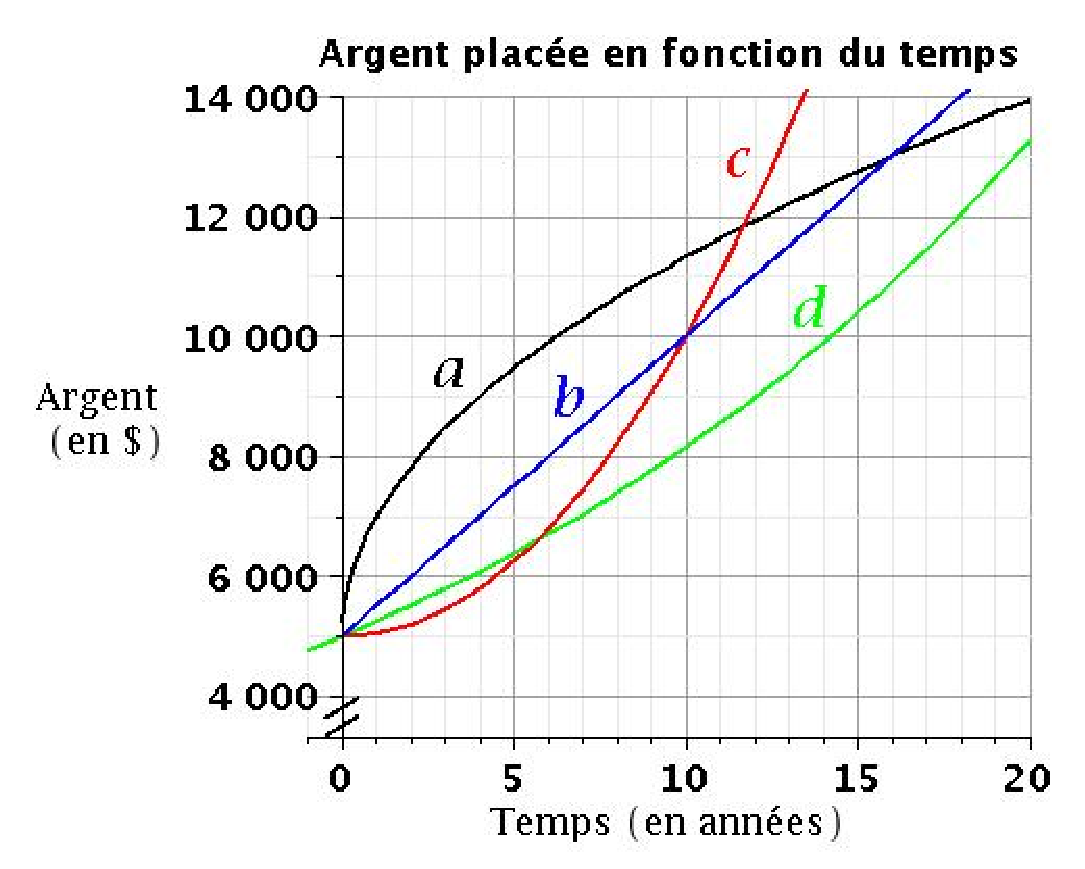
\includegraphics[width=8cm]{fonction184.eps}
 % fonction4.eps: 1048592x1048592 pixel, 0dpi\begin{center}
\end{center}

R\'eponse : d\\

R\'etroaction :\\

We are looking for the curve that represents the situation. Let $y$
be the amount of money and $x$ the time in years. Because the rate
of interest is 5 \% and that the initial amount is 5 000 \$, then
$y=5\,000\left(1,05\right)^{x}$ represents the situation.\\

The relation is exponential. It is then a curve that grows steeper
with time. That can be either $c$ or $d$.\\
We can calculate the amount after ten years to find the good one.
\begin{eqnarray*}
y&=& 5\,000\left(1,05\right)^{x}\\
&=& 5\,000\left(1,05\right)^{10}\\
&=& 5\,000\times 1,6289\\
&=& 8144,47
\end{eqnarray*}
Because $\left(10,\,\,8144,47\right)$ is right on the $d$ line, it
is the good one.
\begin{center}
 \includegraphics[width=8cm]{fonction184.eps}
 % fonction4.eps: 1048592x1048592 pixel, 0dpi\begin{center}
\end{center}
Therefore, the answer is d.\\

4185-- The head of a great company wants to build a phone chain to
reach all the $20\,000$ employees. She will call three employees
that will do the same and so on. She wants to represent the relation
between the group number of people calling and the number of people
reached by them. As an example, she is the first group and
the three people she is reaching are the second group.\\

True or false?\\
The following graphic represents the situation.
\begin{center}
 \includegraphics[width=9cm]{fonction185.eps}
 % fonction4.eps: 1048592x1048592 pixel, 0dpi\begin{center}
\end{center}

R\'eponse : True\\

R\'etroaction :\\

We want to know if the graphic:
\begin{center}
 \includegraphics[width=9cm]{fonction185.eps}
 % fonction4.eps: 1048592x1048592 pixel, 0dpi\begin{center}
\end{center}
represents the situation:\\
The head calls three employees that each call three other and so on.\\

We can build a table of values.
\begin{center}
\begin{tabular}{ |l|l|}
\hline
Group number & Number of people reached\\
\hline
1 & 3\\
2 & 9\\
3 & 27\\
4 & 81\\
5 & 243\\
\hline
\end{tabular}
\end{center}

When the group number raises by one, the number of people reached is
multiplied by three. The relation is then an exponential of base
$3$, $y=3^x$. That is what's shown on the graphic. Lets try at
$x=8$:
\begin{eqnarray*}
y&=&3^x\\
&=&3^8\\
&=&6\,561
\end{eqnarray*}
The point $\left(8,\,\,6\,561\right)$ is part of the curve.\\
Therefore, the answer is : true.\\


4195-- True or false?\\
The following graphs represent the same situation:
\begin{center}
\begin{tabular}{c c}
\includegraphics[width=5cm]{arith195.1.eps}
% alg80.1.eps : 300dpi, width=3.39cm, height=3.39cm, bb=0 0 400 400
&\includegraphics[width=5cm]{arith195.2.eps}
% alg80.1.eps : 300dpi, width=3.39cm, height=3.39cm, bb=0 0 400 400\\
\end{tabular}
\end{center}
R\'eponse: True\\

R\'etroaction:\\

We are wondering if both graphs are the same and they are.
\begin{center}
\begin{tabular}{l l}
\includegraphics[width=5cm]{arith195.1.eps}
% alg80.1.eps : 300dpi, width=3.39cm, height=3.39cm, bb=0 0 400 400
&\includegraphics[width=5cm]{arith195.2.eps}
% alg80.1.eps : 300dpi, width=3.39cm, height=3.39cm, bb=0 0 400 400\\
\end{tabular}
\end{center}
The graphs' summits are the same just like their edges.\\
Therefore, the answer is : true.\\

4196-- A \underline{\qquad\qquad} is an edge having both ends on the
same vertex.\\

R\'eponse: loop\\

R\'etroaction:\\

We are looking for the name that represents an edge having both ends
on the same vertex.\\

That definition is one of a loop.\\
Therefore, the answer is loop.\\

4197-- Put the words at the right place.

The \underline{1.\qquad\qquad} of a \underline{2.\qquad\qquad} is
the number of times that an \underline{3.\qquad\qquad} touches that \underline{4.\qquad\qquad}.\\

a$)$ 1.degree, 2.edge, 3.edge, 4.vertex\\
b$)$ 1.degree, 2.vertex, 3.edge, 4.vertex\\
c$)$ 1.vertex, 2.edge, 3.edge, 4.vertex\\
d$)$ 1.vertex, 2.edge, 3.vertex, 4.degree\\

R\'eponse: b$)$\\

R\'etroaction:\\

We are looking the words to complete the definition:\\
The \underline{degree} of a \underline{vertex} is the number of
times an \underline{edge} touches that \underline{vertex}.\\
Therefore, the answer is b$)$.\\


4202-- A complete graph is:\\

a$)$ a graph in which all points are linked to the others.\\
b$)$ a graph that has the shape of a regular polygon.\\
c$)$ a graph that has as many loops as vertexes.\\
d$)$ a graph without loops that has all the possible edges to link
only once all vertexes.\\

R\'eponse: d$)$\\

R\'etroaction:\\

A complete graph is a graph without loops that has all the possible
edges to link only once all vertexes.\\
The answer a$)$ is not complete and b$)$ and c$)$ are wrong.\\
Therefore, the answer is d$)$.\\


4207-- Which of the following graphs is directed?
\begin{center}
\begin{tabular}{l l}
a$)$ & b$)$\\
\includegraphics[width=7cm]{arith201.1.eps}
% alg80.1.eps : 300dpi, width=3.39cm, height=3.39cm, bb=0 0 400 400
& \includegraphics[width=7cm]{arith207.2.eps}\\
% alg80.2.eps : 300dpi, width=3.39cm, height=3.39cm, bb=0 0 400 400
c$)$ & d$)$\\
\includegraphics[width=7cm]{arith207.3.eps}
% alg80.3.eps : 300dpi, width=3.39cm, height=3.39cm, bb=0 0 400 400
& \includegraphics[width=7cm]{arith207.4.eps}\\
% alg80.4.eps : 300dpi, width=3.39cm, height=3.39cm, bb=0 0 400 400
\end{tabular}
\end{center}
R\'eponse: d$)$\\

R\'etroaction:\\

We are looking for an directed graph among these:
\begin{center}
\begin{tabular}{l l}
\includegraphics[width=7cm]{arith201.1.eps}
% alg80.1.eps : 300dpi, width=3.39cm, height=3.39cm, bb=0 0 400 400
& \includegraphics[width=7cm]{arith207.2.eps}\\
% alg80.2.eps : 300dpi, width=3.39cm, height=3.39cm, bb=0 0 400 400
\includegraphics[width=7cm]{arith207.3.eps}
% alg80.3.eps : 300dpi, width=3.39cm, height=3.39cm, bb=0 0 400 400
& \includegraphics[width=7cm]{arith207.4.eps}\\
% alg80.4.eps : 300dpi, width=3.39cm, height=3.39cm, bb=0 0 400 400
\end{tabular}
\end{center}
The only directed graph among those is the last one.\\
The first one is not directed because it only contains edges. The
second one is not even a graph because two of its vertexes have the
same name. The third is mixed because it contains an edge, a loop
and arcs. The last one is directed because it contains only arcs.\\
Therefore, the answer is d$)$.\\


4214-- Here's the map of the corridors of a school's first floor.
\begin{center}
 \includegraphics[width=7cm]{arith214.eps}
% alg80.1.eps : 300dpi, width=3.39cm, height=3.39cm, bb=0 0 400 400\\
\end{center}
What is the place where the traffic is the greatest during
displacement in that school?\\

R\'eponse: C\\

R\'etroaction:\\

\begin{center}
 \includegraphics[width=7cm]{arith214.eps}
% alg80.1.eps : 300dpi, width=3.39cm, height=3.39cm, bb=0 0 400 400\\
\end{center}
The place where the traffic is the greatest in a school is where the
most corridors meet. So the vertex having the greatest degree is the
one. It is the vertex
$C$ (d$(C)=4$) because the other vertexes have degrees lower than four.\\
Therefore, the answer is c.\\


4217-- True or false?\\
There is a chain between A and D in the following graph:
\begin{center}
 \includegraphics[width=7cm]{arith194.eps}
% alg80.1.eps : 300dpi, width=3.39cm, height=3.39cm, bb=0 0 400 400\\
\end{center}

R\'eponse: True\\

R\'etroaction:\\

Is there or not a chain between A and D on
\begin{center}
 \includegraphics[width=7cm]{arith194.eps}
% alg80.1.eps : 300dpi, width=3.39cm, height=3.39cm, bb=0 0 400 400\\
\end{center}
A chain is a series of vertexes for which there is always an edge
between consecutive vertexes.\\
The vertexes A and D on the graph are linked by an edge. So the next
series is a chain: $\left(A, D, A, D\right)$. There is also:
$\left(A, D, C, D\right)$ and many others.\\
Therefore, the answer is: true.\\

4218-- Which of the following series is not a chain on the graph?
\begin{center}
 \includegraphics[width=7cm]{arith201.1.eps}
% alg80.1.eps : 300dpi, width=3.39cm, height=3.39cm, bb=0 0 400 400\\
\end{center}

a$)$ $\left(A, C, D, B, D, F\right)$\\
b$)$ $\left(A, C, D, C, D, F, F\right)$\\
c$)$ $\left(A, D, C, D, C, F\right)$\\
d$)$ $\left(F, F, D, C, A, D, B\right)$\\

R\'eponse: c$)$\\

R\'etroaction:\\

We are looking for the series that is not a chain on the graph:
\begin{center}
 \includegraphics[width=7cm]{arith201.1.eps}
% alg80.1.eps : 300dpi, width=3.39cm, height=3.39cm, bb=0 0 400 400\\
\end{center}
A chain is a series of vertexes for which there is always an edge
between consecutive vertexes.\\
The only chain that is wrong is $\left(A, D, C, D, C, F\right)$
because there is no edge between vertexes C and F. Take note that
the loop in F allows to go from F to F so $\left(F, F, F\right)$ can
be a chain.\\
Therefore, the answer is c$)$.\\


4221-- Which of the following series is simple cycle of this graph?
\begin{center}
 \includegraphics[width=7cm]{arith201.1.eps}
% alg80.1.eps : 300dpi, width=3.39cm, height=3.39cm, bb=0 0 400 400\\
\end{center}

a$)$ $\left(A, C, D, F, D, A\right)$\\
b$)$ $\left(B, D, C, D, A\right)$\\
c$)$ $\left(C, D, C, D, A, C\right)$\\
d$)$ $\left(D, F, E, A, C, D\right)$\\

R\'eponse: c$)$\\

R\'etroaction:\\

We are looking for the simple cycle among:
\begin{center}
 $\left(A, C, D, F, D, A\right)$\\
 $\left(B, D, C, D, A\right)$\\
 $\left(C, D, C, D, A, C\right)$\\
 $\left(D, F, E, A, C, D\right)$\\
\end{center}
\begin{center}
 \includegraphics[width=7cm]{arith201.1.eps}
% alg80.1.eps : 300dpi, width=3.39cm, height=3.39cm, bb=0 0 400 400\\
\end{center}
A simple cycle is a cycle in which all edges are different.
\begin{itemize}
\item The series a$)$ is a cycle but not a simple one because it
goes twice on the edge $\{D, F\}$.

\item The series b$)$ is a chain. It is not a cycle because it doesn't come back at the start.

\item The series c$)$ is a simple cycle because all its edges are different. In fact, the edge $\{C,
D\}$ is there three times, but notice that there are three edges
between vertexes $C$ and $D$. So a different one is taken each
time.

\item The series d$)$ is not a chain because there is no edge between vertexes $E$ and $F$ and then between $A$
and $E$.
\end{itemize}
So the simple cycle is $\left(C, D, C, D, A, C\right)$.\\
Therefore, the answer is c$)$.\\

4222-- In a \underline{\qquad\qquad} graph, there is a simple cycle
that goes on all edges.\\

a$)$ connected\\
b$)$ mixed\\
c$)$ Eulerian\\
d$)$ directed\\

R\'eponse: c$)$\\

R\'etroaction:\\

In an \underline{Eulerian} graph, there is a simple cycle that goes
on all edges. In fact, the cycle goes on each edge only one time.\\
Therefore, the answer is c$)$.\\

4223-- A connected graph has for vertexes the four following points:
A, B, C and D where d$($A$)=3$, d$($B$)$=d$($C$)=2$ and d$($D$)=1$.
Is it possible for the graph to be Eulerian? Yes or no.\\

R\'eponse: no\\

R\'etroaction:\\

Is possible or not for a graph that has vertexes A, B, C and D with
d$($A$)=3$, d$($B$)$=d$($C$)=2$ and
d$($D$)=1$ to be Eulerian?\\

For a graph to be Eulerian, there's got to be a simple cycle that
goes on all edges. So the degree of each vertex has to be even
because a cycle arriving at a vertex has to leave it.\\

In the situation, the degrees of all vertexes are not all even so
the graph is not Eulerian.\\
Therefore, the answer is no.\\


4225-- Jackie arrives at the camping she is spending the weekend at
with her friend Stan. She doesn't know where her friend is set so
she decides to check all the way around for him. She wishes to go in
all the streets without ever going twice on the same one. Is it
possible if she is in car and has to respect the one ways?
\begin{center}
 \includegraphics[width=7cm]{arith225.eps}
% alg80.1.eps : 300dpi, width=3.39cm, height=3.39cm, bb=0 0 400 400\\
\end{center}

R\'eponse: no\\

R\'etroaction:\\

Is it possible to pass on all streets but not twice?
\begin{center}
 \includegraphics[width=7cm]{arith225.eps}
% alg80.1.eps : 300dpi, width=3.39cm, height=3.39cm, bb=0 0 400 400\\
\end{center}
Because the arcs $[A, B]$, $[A, B]$, $[C, B]$ and $[C, D]$ are all
one ways that go in the same direction, it is impossible to pass in
all streets only once while respecting the roadsigns.\\
Therefore, the answer is no.\\


4269-- What linear correlation coefficient is appropriate for this
scatter plot?
\begin{center}
 \includegraphics[width=7cm]{stt253.1.eps}
 % alg77.eps: 1048592x1048592 pixel, 0dpi\begin{center}
\end{center}

a$)$ $-0,77$\\
b$)$ $-0,4$\\
c$)$ 0 \\
d$)$ $0,77$\\

R\'eponse: d$)$\\

R\'etroaction:\\

\begin{center}
 \includegraphics[width=7cm]{stt253.1.eps}
 % alg77.eps: 1048592x1048592 pixel, 0dpi\begin{center}
\end{center}
The scatter plot has a strong positive linear correlation. Its
linear correlation coefficient is then close to 1. It is
$0,77$.\\
Therefore, the answer is d$)$.\\

4270-- What linear correlation coefficient is appropriate for this
scatter plot?
\begin{center}
 \includegraphics[width=7cm]{stt253.2.eps}
 % alg77.eps: 1048592x1048592 pixel, 0dpi\begin{center}
\end{center}

a$)$ $-0,98$\\
b$)$ $-0,67$\\
c$)$ 0 \\
d$)$ $0,67$\\

R\'eponse: a$)$\\

R\'etroaction:\\

\begin{center}
 \includegraphics[width=7cm]{stt253.2.eps}
 % alg77.eps: 1048592x1048592 pixel, 0dpi\begin{center}
\end{center}
The scatter plot has a near perfect negative linear correlation. Its
linear correlation coefficient is then close to -1. It is $-0,98$.\\
Therefore, the answer is a$)$.\\


4272-- In order to calculate the correlation coefficient of a
scatter plot, Chelsea has traced the smallest possible rectangle
around the plot. She says the correlation is positive and that the
rectangle is three times longer than wide. What is the correlation
coefficient of that scatter plot?\\

a$)$ $-0,67$\\
b$)$ $0,33$\\
c$)$ $0,67$\\
d$)$ 1\\

R\'eponse: c$)$\\

R\'etroaction:\\

We are looking for the linear correlation coefficient of a scatter
plot which correlation is positive and for which the rectangle is
three times longer than wide.\\

Let $x$ be the width of the rectangle. The length is then $3x$.
Here's the coefficient calculation:
\begin{eqnarray*}
\pm\left(1-\frac{\textnormal{size of the small
side}}{\textnormal{size of the large side}}\right)
&=&+\left(1-\frac{x}{3x}\right)\\
&=&+\left(1-\frac{1}{3}\right)\\
&=&+\left(\frac{3}{3}-\frac{1}{3}\right)\\
&=&+\left(\frac{2}{3}\right)\\
&=&+0,67
\end{eqnarray*}
Therefore, the answer is c$)$.\\

4273-- In order to calculate the correlation coefficient of a
scatter plot, Chelsea has traced the smallest possible rectangle
around the plot. She says the correlation is negative and that the
rectangle is four times longer than wide. What the correlation
coefficient of that scatter plot?\\

a$)$ $-1$\\
b$)$ $-0,75$\\
c$)$ $-0,25$\\
d$)$ $0,75$\\

R\'eponse: b$)$\\

R\'etroaction:\\

We are looking for the linear correlation coefficient of a scatter
plot which correlation is negative and for which the rectangle is
four times longer than wide.\\

Let $x$ be the width of the rectangle. The length is then $4x$.
Here's the coefficient calculation:
\begin{eqnarray*}
\pm\left(1-\frac{\textnormal{size of the small
side}}{\textnormal{size of the large side}}\right)
&=&-\left(1-\frac{x}{4x}\right)\\
&=&-\left(1-\frac{1}{4}\right)\\
&=&-\left(\frac{4}{4}-\frac{1}{4}\right)\\
&=&-\left(\frac{3}{4}\right)\\
&=&-0,75
\end{eqnarray*}
Therefore, the answer is b$)$.\\


4281-- Joe rolls a dice having a red face, two blue faces, four
white faces and five yellow faces. The
possible universe of that experiment is:\\

a$)$ \{1, 2, 4, 5\}\\
b$)$ \{1, 2, 3, 4, 5, 6, 7, 8, 9, 10, 11, 12\}\\
c$)$ \{A, B, C, D, E, F\}\\
d$)$ \{white, blue, yellow, red\}\\

R\'eponse: d$)$\\

R\'etroaction:\\

Joe rolls a dice having a ref face, two blue faces, four white faces
and five yellow faces. We are looking for the possible universe of
that experiment.\\


The faces of the dice are not numbered nor identified by letters,
they are of different colors. So the events are the possible colors.
The possible universe $\Omega$ is the set of all results that can
occur. $\Omega=\{\textnormal{white, blue, yellow, red}\}$\\
Therefore, the answer is d$)$.\\


4283-- Amy rolls twice a dice having a red face, two blue faces,
four white faces and five yellow faces. What is the probability for
Amy to get a blue face followed by a yellow face? The answer has to
e rounded to the tenth.\\

R\'eponse: 0,07\\

R\'etroaction:\\

We are looking for the probability to get a blue face followed by a
yellow face. The dice has a red face, two blue faces, four white
faces and five yellow faces.
\begin{eqnarray*}
\textnormal{P(blue and yellow)}&=&\textnormal{P(blue)}\times
\textnormal{P(yellow)}\\
&=&\frac{\textnormal{number of positive blue
events}}{\textnormal{number of possible events}} \times
\frac{\textnormal{number of positive yellow events}}{\textnormal{number of possible events}}\\\\
&=&\frac{2}{12}\times\frac{5}{12}\\
&=&\frac{1}{6}\times\frac{5}{12}\\
&=&\frac{5}{72}\\
&\approx&0,07
\end{eqnarray*}
So the probability for the two events to occur in that order is $0,07$.\\
Therefore, the answer is $0,07$.\\


4305-- You pay 2 \$ at a game of chance that is fair. By playing
only once, it is possible to win one of the two prizes. The
probability to win 10 \$ at this game is $0,1$. What has to be the
value of the other prize so that the probability of winning it
is $0,05$?\\

a$)$ 20 \$\\
b$)$ 25 \$\\
c$)$ 30 \$\\
d$)$ 50 \$\\

R\'eponse: a$)$\\

R\'etroaction:\\

You pay 2 \$ at a game of chance that is fair. By playing only once,
it is possible to win one of the two prizes. The probability to win
10 \$ at this game is $0,1$. We are looking for the value of the
other prize so that the probability of winning it is $0,05$.\\

A game is fair when the mathematical expectation is equal to the
cost of the game. We then want the expectation to be 2 \$.
\begin{eqnarray*}
\textnormal{Mathematical expectation}&=&\textnormal{P(A})\times
g(\textnormal{A})+\textnormal{P(B})\times
g(\textnormal{B})\\
2\,\$ &=& 0,1 \times 10\,\$ + 0,05\times
g(\textnormal{B})\\
2\,\$ &=& 1\,\$ + 0,05\times g(\textnormal{B})\\
1\,\$ &=& 0,05\times g(\textnormal{B})\\
20\,\$ &=& g(\textnormal{B})
\end{eqnarray*}
The value of the other prize has to be 20 \$.\\
Therefore, the answer is a$)$.\\

4306-- Joe pays 3 \$ at a game of chance. He has to toss a coin and
pick to marbles out of a bag containing two red, three yellow and
five blue marbles.\\
The following tree represents the situation.
\begin{center}
 \includegraphics[width=15cm]{stt285.eps}
 % alg77.eps: 1048592x1048592 pixel, 0dpi\begin{center}
\end{center}
The only prize for this game is 15 \$ and to win it, Joe has to get
tails and two marbles of the same color. Is that game fair?
Yes or no.\\

R\'eponse: no\\

R\'etroaction:\\

Is the game fair?.\\
Joe pays 3 \$ to toss a coin and pick to marbles out of a bag
containing two red, three yellow and five blue marbles.
\begin{center}
 \includegraphics[width=15cm]{stt285.eps}
 % alg77.eps: 1048592x1048592 pixel, 0dpi\begin{center}
\end{center}
To get the only prize of 15 \$ he has to get tails at the toss and
get the marbles of the same color.\\

A game is fair when the mathematical expectation is equal to the
cost of the game.
\begin{eqnarray*}
\textnormal{Mathematical expectation}&=&\textnormal{P(A})\times
g(\textnormal{A})\\
&=& \left(\textnormal{P(tails and 2 red})+\textnormal{P(tails and 2
yellow})+\textnormal{P(tails and 2 blue})\right)\times\,15\, \$\\
&=&\left(0,5\times0,2\times0,11+0,5\times0,3\times0,22+0,5\times0,5\times0,44\right)\times\,15\,\$\\
&=&\left(0,011+0,033+0,11\right)\times\,15\,\$\\
&=& 0,154\times 15\,\$\\
&=& 2,31\,\$
\end{eqnarray*}
So the expectation is $2,31$ \$. Because the cost of a game is 3
\$ and the expectation \mbox{$2,31$ \$}, the game is not fair.\\
Therefore, the answer is no.\\


4308--Your best friend invites you at a party at his place. He is
planning a game of chance for the night. He wants to build a wheel
that has five zones like this one:
\begin{center}
 \includegraphics[width=7cm]{stt308.eps}
 % alg77.eps: 1048592x1048592 pixel, 0dpi\begin{center}
\end{center}
He wants two of the zones to be prize-winning and doesn't want to
raise any money from the game. He asks 1 \$ per player. The red zone
is a win one and the prize is 5 \$. What zone must be the other
winning one so its prize is $3,50$ \$?\\

a$)$ the blue one\\
b$)$ the yellow one\\
c$)$ the orange one\\
d$)$ the green one\\

R\'eponse : b$)$\\

R\'etroaction:\\

The situation:\\
Your friend wants to build a five zones wheel like this one:
\begin{center}
 \includegraphics[width=7cm]{stt308.eps}
 % alg77.eps: 1048592x1048592 pixel, 0dpi\begin{center}
\end{center}
He wants it to have zones to be prize-winning and wants no profits.
He asks 1 \$ per player. The red zone is worth 5 \$. What other zone
should a winning one if its prize is $3,50$ \$.\\

A game is fair when the mathematical expectation is equal to the
cost of the game.
\begin{eqnarray*}
\textnormal{Mathematical expectation}&=&\textnormal{P(red})\times
g(\textnormal{red})+\textnormal{P(B})\times
g(\textnormal{B})\\
1
\,\$&=&\left(1-\left(\frac{1}{4}+\frac{1}{8}+\frac{3}{8}+\frac{1}{6}\right)\right)\times
5\,\$+P(\textnormal{B})\times 3,5\,\$\\
1
\,\$&=&\left(1-\left(\frac{6}{24}+\frac{3}{24}+\frac{9}{24}+\frac{4}{24}\right)\right)\times
5\,\$+\textnormal{P(B})\times 3,5\,\$\\
1\,\$&=&\left(\frac{24}{24}-\left(\frac{22}{24}\right)\right)\times
5\,\$+\textnormal{P(B})\times 3,5\,\$\\
1\,\$&=&\left(\frac{2}{24}\right)\times
5\,\$+\textnormal{P(B})\times 3,5\,\$\\
1\,\$&=&\left(\frac{1}{12}\right)\times
5\,\$+\textnormal{P(B})\times 3,5\,\$\\
1\,\$&=& \frac{5}{12}\,\$+\textnormal{P(B})\times 3,5\,\$\\
\frac{12}{12}\,\$-\frac{5}{12}\,\$&=& \textnormal{P(B})\times 3,5\,\$\\
\frac{7}{12}\,\$&=& \textnormal{P(B})\times 3,5\,\$\\
\frac{\frac{7}{12}}{3,5} &=& \textnormal{P(B})\\
\frac{\frac{7}{12}}{\frac{7}{2}} &=& \textnormal{P(B})\\
\frac{1}{6} &=& \textnormal{P(B})
\end{eqnarray*}
The probability of winning $3,50$ \$ has to be $\frac{1}{6}$ so that
the game is fair. The zone worth a prize of $3,50$ \$ has to be the yellow one.\\
Therefore, the answer is b$)$.\\


4310-- During a party, Emily is wondering wether or not she should
play a game chance suggested by her friend. To play, she must pay 3
\$. The game consists in picking a piece of paper from a box. In
that box, one piece has 10 \$ written on it, three have 5 \$ and
four
have 2 \$ on them. What following statement is true?\\

a$)$ There is more profit to come for the organizer than the player.\\
b$)$ There is more profit to come for the player than the organizer.\\
c$)$ The game is fair.\\
d$)$ The game is unfair, it's not worth playing.\\

R\'eponse: b$)$\\

R\'etroaction:\\

Is the game fair? If not, who is it most profitable for.\\

A game is fair when the mathematical expectation is equal to the
cost of the game.
\begin{eqnarray*}
\textnormal{Mathematical expectation}&=&\textnormal{P(10 \$})\times
g(\textnormal{10 \$})+\textnormal{P(5 \$})\times
g(\textnormal{10 \$})+\textnormal{P(2 \$})\times g(\textnormal{2 \$})\\
&=& 0,125 \times 10\,\$+ 0,375 \times 5\,\$+0,5\times 2\,\$\\
&=& 1,25\,\$+ 1,875\,\$+1\,\$\\
&=&4,125\,\$\\
&>&3\,\$
\end{eqnarray*}
The game is not fair. Because the profit expectation is greater than
the cost of the game, there is more profit to come in playing than
organizing. In fact, her friend will not make profit and will have
to pay for the ones playing.\\
Therefore, the answer is b$)$.\\


4312-- A game of chance goes like this. You have to pay 6 \$ and you
roll three dices whose six faces are numbered from 1 to 6. You win
80 \$ for having three 6, 20 \$ for having three identical faces
other than 6 and 10 \$ if you get two identical faces. Otherwise,
you don't win. If you play 10 times, what amount is it reasonable to
hope getting in return?\\

a$)$ 0 \$\\
b$)$ 5 \$\\
c$)$ 22,22 \$\\
d$)$ 50 \$\\

R\'eponse: d$)$\\

R\'etroaction:\\

In order to play the game, you have to pay 6 \$ and you roll three
dices whose six faces are numbered from 1 to 6. You win 80 \$ for
having three 6, 20 \$ for having three identical faces other than 6
and 10 \$ if you get two identical faces. Otherwise, you don't win.
We are wondering what amount is reasonable to hope getting in return
if you play 10 times. We want the mathematical expectation of the
game. Because you play ten times, multiply the expectation by ten.
\begin{eqnarray*}
\textnormal{P(three 6})&=&\textnormal{P(6})\times \textnormal{P(6})\times \textnormal{P(6})\\
&=&\left(\frac{1}{6}\times\frac{1}{6}\times\frac{1}{6}\right)\\
&=& \frac{1}{216}
\end{eqnarray*}
\begin{eqnarray*}
P(\textnormal{three identical faces other than
6})&=&\textnormal{P(other than 6})\times \textnormal{P(same as the
first one})\times \textnormal{P(same as the first one)}\\
&=&\left(\frac{5}{6}\times\frac{1}{6}\times\frac{1}{6}\right)\\
&=& \frac{5}{216}
\end{eqnarray*}
There is three ways of getting two identical faces and one
different. It can be X, X, Y where X and Y are different:
\begin{eqnarray*}
\textnormal{P(X, X, Y})&=&\textnormal{P(X})\times \textnormal{P(X}|\textnormal{X)}\times \textnormal{P(Y}|
\textnormal{X})\\
&=&\left(\frac{6}{6}\times\frac{1}{6}\times\frac{5}{6}\right)\\
&=& \frac{30}{216}
\end{eqnarray*}
It can be X, Y, Y where X and Y are different:
\begin{eqnarray*}
\textnormal{P(X, Y, X})&=&\textnormal{P(X})\times \textnormal{P(Y}|\textnormal{X})\times \textnormal{P(X}|
\textnormal{X})\\
&=&\left(\frac{6}{6}\times\frac{5}{6}\times\frac{1}{6}\right)\\
&=& \frac{30}{216}
\end{eqnarray*}
It can be Y, X, X where X and Y are different:
\begin{eqnarray*}
\textnormal{P(Y, X, X})&=&\textnormal{P(Y})\times \textnormal{P(X}|\textnormal{Y})\times \textnormal{P(X}|
\textnormal{X})\\
&=&\left(\frac{6}{6}\times\frac{5}{6}\times\frac{1}{6}\right)\\
&=& \frac{30}{216}
\end{eqnarray*}
\begin{eqnarray*}
\textnormal{Mathematical expectation}&=&\textnormal{P(three
6})\times
g(\textnormal{three 6})\\
& &+\textnormal{P(three identical faces other than 6})\times
g(\textnormal{three identical faces other than 6})\\
& &+\textnormal{P(two identical and one different})\times
g(\textnormal{two identical and one different})\\
&=&\frac{1}{216}\times 80\,\$+\frac{5}{216}\times
20\,\$+\left(\frac{30}{216}+\frac{30}{216}+\frac{30}{216}\right)\times 10\,\$\\
&=&\frac{1}{216}\times 80\,\$+\frac{5}{216}\times20\,\$+\frac{90}{216}\times 10\,\$\\
&=&\frac{80}{216}\,\$+\frac{100}{216}\,\$+\frac{900}{216}\,\$\\
&=&\frac{1080}{216}\,\$\\
&=&5\,\$
\end{eqnarray*}
So the expectation is 5 \$. You can then play and hope
winning 5 \$ $\times$ 10 $=$ 50 \$ by playing ten times.\\
Therefore, the answer is d$)$.\\


4314-- Gabriel said to Fred that the distance between $A$ and $B$ on
the drawing is represented by the expression $d(A, B)=\sqrt{15+10}$.
\begin{center}
 \includegraphics[width=5cm]{geo314.eps}
 % alg77.eps: 1048592x1048592 pixel, 0dpi\begin{center}
\end{center}
Is he right? Yes or no.\\

R�ponse : no\\

R\'etroaction:\\

Gabriel is wrong. The distance between $A$ and $B$ is not
represented by $d(A, B)=\sqrt{15+10}$.
\begin{center}
 \includegraphics[width=5cm]{geo314.eps}
 % alg77.eps: 1048592x1048592 pixel, 0dpi\begin{center}
\end{center}

The triangle is right angled and with Pythagoras' relation we have:
\begin{eqnarray*}
d(A, B)^2&=&d(A, C)^2+d(B, C)^2\\
d(A, B)&=&\sqrt{15^2+10^2}\\
d(A, B)&=&\sqrt{225+100}\\
d(A, B)&=&\sqrt{325}
\end{eqnarray*}
Gabriel forgot to square the length of the catheti.\\
Therefore, the answer is no.\\

4316-- On the following map we see Ann's(A), Bernard's(B),
Charles'(C), Dan's(D), Erica's(E) and Fanny's(F) houses.
\begin{center}
 \includegraphics[width=6cm]{geo315.eps}
 % alg77.eps: 1048592x1048592 pixel, 0dpi\begin{center}
\end{center}
By going through the streets, who lives the closest to Charles?
Answer with a letter.\\

R�ponse : D\\

R\'etroaction:\\

We are wondering who lives the closest to Charles only going through
the streets.
\begin{center}
 \includegraphics[width=6cm]{geo315.eps}
 % alg77.eps: 1048592x1048592 pixel, 0dpi\begin{center}
\end{center}
Dan is the one living the closest to Charles because he lives three
units away while the others live four or five units away from
him.\\
Therefore, the answer is D.\\


4334-- Carl wants to go to Melissa's place and wants to go by the
river to pick up a flower. To get there, he has to go through a
large field. Melissa lives at A and Carl lives at B. What has to be
the value of
$x$ so Carl can get there the soonest possible?\\
Round to the tenth.
\begin{center}
 \includegraphics[width=7cm]{geo333.eps}
 % alg77.eps: 1048592x1048592 pixel, 0dpi\begin{center}
\end{center}
R\'eponse: 3,1\\

R\'etroaction:\\

Carl wants to get there the soonest possible so he takes the
shortest path that passes aside the river. The shortest path is the
straight line. We have to find the value of $x$ so A, C and
B$^\prime$ are aligned.
\begin{center}
 \includegraphics[width=7cm]{geo334.eps}
 % alg77.eps: 1048592x1048592 pixel, 0dpi\begin{center}
\end{center}
Let A, C and B$^\prime$ be aligned. The triangles are the same
because they share opposite apexes angles and both have a right
angle. We find $x$ with the ratio of homologous sides of similar
triangle.
\begin{eqnarray*}
\frac{5}{4}&=&\frac{7-x}{x}\\
5x&=&4(7-x)\\
5x&=&28-4x\\
9x&=&28\\
x&=&\frac{28}{9}\\
x&\approx&3,1
\end{eqnarray*}
Therefore, the answer is $3,1$.\\

4335-- Jenny is out for a walk with her mother Suzanne. At $A$ on
their trip, they get to chose among two path to get to $B$. From
$A$, Jenny takes the long road and runs at nine kilometers an hour
while her mother is quick marching at six kilometer an hour on the
other road. What must be the length of $\overline{AC}$ in meters so
Suzanne and Jenny arrive at the same time at $B$?
\begin{center}
 \includegraphics[width=7cm]{geo335.eps}
 % alg77.eps: 1048592x1048592 pixel, 0dpi\begin{center}
\end{center}

R\'eponse: 900\\

R\'etroaction:\\
\begin{center}
 \includegraphics[width=7cm]{geo335.eps}
 % alg77.eps: 1048592x1048592 pixel, 0dpi\begin{center}
\end{center}
We want both people to get to $B$ at the same time.\\

Suzanne does 1000 m at 6 km/h $=$ 6 000 m/h. It then takes her $10$
minutes to get to B.
\begin{eqnarray*}
\frac{60\textnormal{ min}}{6\,000\textnormal{
m}}&=&\frac{x}{1\,000\textnormal{ m}}\\
\frac{60\textnormal{ min}\times1\,000\textnormal{
m}}{6\,000\textnormal{
m}}&=&x\\
10\textnormal{ min}&=&x
\end{eqnarray*}

Jenny runs at a speed of 9 km/h $=$ 9 000 m/h and she has to get to
B in 10 minutes. She does $1\,500$ m.
\begin{eqnarray*}
\frac{9\,000\textnormal{
m}}{60\textnormal{ min}}&=&\frac{x}{10\textnormal{ min}}\\
\frac{9\,000\textnormal{
m}\times10\textnormal{ min}}{60\textnormal{ min}}&=&x\\
1\,500\textnormal{ m}&=&x
\end{eqnarray*}

Because
m$\overline{BC} = 600$ m, then m$\overline{AC} = 1\,500$ m $-\,600$ m $=900$ m.\\
Therefore, the answer is 900.\\

4336-- Jenny is out for a walk with her mother Suzanne. At $A$ on
their trip, they get to chose among two path to get to $B$. From
$A$, Jenny takes the long road and runs at nine kilometers an hour
while her mother is quick marching at six kilometer an hour on the
other road. What must be the length of $\overline{CB}$ in meters so
Suzanne and Jenny arrive at the same time at $B$?
\begin{center}
 \includegraphics[width=7cm]{geo336.eps}
 % alg77.eps: 1048592x1048592 pixel, 0dpi\begin{center}
\end{center}

R\'eponse: 600\\

R\'etroaction:\\
\begin{center}
 \includegraphics[width=7cm]{geo336.eps}
 % alg77.eps: 1048592x1048592 pixel, 0dpi\begin{center}
\end{center}
We want both people to get to $B$ at the same time.\\

Suzanne does 1000 m at 6 km/h $=$ 6 000 m/h. It then takes her $10$
minutes to get to B.
\begin{eqnarray*}
\frac{60\textnormal{ min}}{6\,000\textnormal{
m}}&=&\frac{x}{1\,000\textnormal{ m}}\\
\frac{60\textnormal{ min}\times1\,000\textnormal{
m}}{6\,000\textnormal{
m}}&=&x\\
10\textnormal{ min}&=&x
\end{eqnarray*}

Jenny runs at a speed of 9 km/h $=$ 9 000 m/h and she has to get to
B in 10 minutes. She does $1\,500$ m.
\begin{eqnarray*}
\frac{9\,000\textnormal{
m}}{60\textnormal{ min}}&=&\frac{x}{10\textnormal{ min}}\\
\frac{9\,000\textnormal{
m}\times10\textnormal{ min}}{60\textnormal{ min}}&=&x\\
1\,500\textnormal{ m}&=&x
\end{eqnarray*}

Because
m$\overline{AC} = 900$ m, then m$\overline{BC} = 1\,500$ m $-\,900$ m $=600$ m.\\
Therefore, the answer is 600.\\

4337-- Jenny is out for a walk with her mother Suzanne. At $A$ on
their trip, they get to chose among two path to get to $B$. From
$A$, Jenny takes the long road and runs at nine kilometers an hour
while her mother is quick marching at six kilometer an hour on the
other road. What must be the angle of $A$ so Suzanne and Jenny
arrive at the same time at $B$?
\begin{center}
 \includegraphics[width=7cm]{geo336.eps}
 % alg77.eps: 1048592x1048592 pixel, 0dpi\begin{center}
\end{center}

a$)$ $30^\circ$\\
b$)$ $32^\circ$\\
c$)$ $33^\circ$\\
d$)$ $36^\circ$\\

R\'eponse: d$)$\\

R\'etroaction:\\
\begin{center}
 \includegraphics[width=7cm]{geo336.eps}
 % alg77.eps: 1048592x1048592 pixel, 0dpi\begin{center}
\end{center}
We want both people to get to $B$ at the same time.\\


Suzanne does 1000 m at 6 km/h $=$ 6 000 m/h. It then takes her $10$
minutes to get at B.
\begin{eqnarray*}
\frac{60\textnormal{ min}}{6\,000\textnormal{
m}}&=&\frac{x}{1\,000\textnormal{ m}}\\
\frac{60\textnormal{ min}\times1\,000\textnormal{
m}}{6\,000\textnormal{
m}}&=&x\\
10\textnormal{ min}&=&x
\end{eqnarray*}

Jenny runs at a speed of 9 km/h $=$ 9 000 m/h and she has to get to
B in 10 minutes. She does $1\,500$ m.
\begin{eqnarray*}
\frac{9\,000\textnormal{
m}}{60\textnormal{ min}}&=&\frac{x}{10\textnormal{ min}}\\
\frac{9\,000\textnormal{
m}\times10\textnormal{ min}}{60\textnormal{ min}}&=&x\\
1\,500\textnormal{ m}&=&x
\end{eqnarray*}

Because
m$\overline{AC} = 900$ m, then m$\overline{BC} = 1\,500$ m $-\,900$ m $=600$ m.\\
Because we know the length of the three sides of the triangle, we
can find the angle $A$ with the cosine law.
\begin{eqnarray*}
a^2&=&b^2+c^2-2bc\cos A\\
600^2&=&900^2+1000^2-2\times900\times1000\times\cos A\\
360\,000&=&810\,000+1\,000\,000-1\,800\,000\times\cos A\\
-1\,450\,000&=&-1\,800\,000\times\cos A\\
\frac{-1\,450\,000}{-1\,800\,000}&=&\cos A\\
\frac{29}{36}&=&\cos A\\
\arccos\left(\frac{29}{36}\right)&=&A\\
36^\circ&\approx&A
\end{eqnarray*}
Therefore, the answer is d$)$.\\

4338-- Jenny is out for a walk with her mother Suzanne. At $A$ on
their trip, they get to chose among two path to get to $B$. From
$A$, Jenny takes the long road and runs at nine kilometers an hour
while her mother is quick marching at six kilometer an hour on the
other road. Who will be waiting for the other at B? Jenny or
Suzanne?
\begin{center}
 \includegraphics[width=7cm]{geo338.eps}
 % alg77.eps: 1048592x1048592 pixel, 0dpi\begin{center}
\end{center}

R\'eponse: Jenny\\

R\'etroaction:\\
\begin{center}
 \includegraphics[width=7cm]{geo338.eps}
 % alg77.eps: 1048592x1048592 pixel, 0dpi\begin{center}
\end{center}
Because the triangle is right angled, we can use the sine and cosine
to find the other sides lengths. Then we can find who will
be waiting for the other at $B$.\\

The segment $\overline{AC}$ measures 800 m.
\begin{eqnarray*}
\cos A &=& \frac{\textnormal{adjacent side}}{\textnormal{hypotenuse}}\\
\cos 36,9^\circ &=& \frac{\overline{AC}}{1000}\\
1000\times \cos 36,9^\circ &=&\overline{AC}\\
800&\approx&\overline{AC}
\end{eqnarray*}
and the segment $\overline{BC}$ measures 600 m.
\begin{eqnarray*}
\sin A &=& \frac{\textnormal{opposite side}}{\textnormal{hypotenuse}}\\
\cos 36,9^\circ &=& \frac{\overline{BC}}{1000}\\
1000\times \cos 36,9^\circ &=&\overline{BC}\\
600&\approx&\overline{BC}
\end{eqnarray*}
The path taken by Jenny is 800 m $+\,600$ m
$=1\,400$ m long.\\

Because Jenny run at 9 km/h and that she must go 1\,400 m, we have:
\begin{eqnarray*}
\frac{9\textnormal{ km}}{1\textnormal{ h}}&=& \frac{1\,400\textnormal{ m}}{x}\\
\frac{9\,000\textnormal{ m}}{60\textnormal{ min}}&=& \frac{1\,400\textnormal{ m}}{x}\\
9\,000\textnormal{ m}\times x &=& 1\,400\textnormal{ m}\times
60\textnormal{ min}\\
x &=& \frac{1\,400\textnormal{ m}\times
60\textnormal{ min}}{9\,000\textnormal{ m}}\\
x &\approx& 9,33 \textnormal{ min}
\end{eqnarray*}
Because Suzanne walks at 6 km/h and that she has to go 1\,000 m, we
have:
\begin{eqnarray*}
\frac{6\textnormal{ km}}{1\textnormal{ h}}&=& \frac{1\,000\textnormal{ m}}{x}\\
\frac{6\,000\textnormal{ m}}{60\textnormal{ min}}&=& \frac{1\,000\textnormal{ m}}{x}\\
6\,000\textnormal{ m}\times x &=& 1\,000\textnormal{ m}\times
60\textnormal{ min}\\
x &=& \frac{1\,000\textnormal{ m}\times
60\textnormal{ min}}{6\,000\textnormal{ m}}\\
x &=& 10 \textnormal{ min}
\end{eqnarray*}
It takes Jenny 9,33 minutes to get to $B$ and 10 minutes to her
mother. Jenny will have to wait $10$ minutes $-9,33$ minutes
$=0,67$ minutes $=40$ seconds before her mother arrives.\\
Therefore, the answer is Jenny.\\

4339--Here's a house lot:
\begin{center}
 \includegraphics[scale=0.40]{geo339.eps}
 % alg77.eps: 1048592x1048592 pixel, 0dpi\begin{center}
\end{center}
The house has a surface of 128 square meters. The paved entrance has
a surface of 80 square meters. The pool is made of two half-circles
and a rectangle because it is 3 meters wide and 10 meters long. What
surface is occupied by the lawn?\\

a$)$ 449,03 m$^2$\\
b$)$ 476 m$^2$\\
c$)$ 685,10 m$^2$\\
d$)$ 1000 m$^2$\\

R\'eponse: a$)$\\

R\'etroaction:\\

We are looking for the surface of the lawn. We know the house
occupies 128 square meters, the paved entrance 80 square meters and
the pool is made of two half-circles and a rectangle. The pool is 3
meter wide and 10 meters long.
\begin{center}
 \includegraphics[scale=0.40]{geo339.eps}
 % alg77.eps: 1048592x1048592 pixel, 0dpi\begin{center}
\end{center}
Before finding the surface, the length of the base of the triangle
has to be found. Because it is a right angled triangle, Pythagoras
relation gives:
\begin{eqnarray*}
a^2+b^2 &=& c^2\\
a^2+10^2&=&24^2\\
a^2+100&=&576\\
a^2&=&476\\
a&\approx&21,82
\end{eqnarray*}

The surface of the lot is:
\begin{eqnarray*}
A_\textnormal{lot} &=&
A_\textnormal{square}+A_\textnormal{triangle}\\
&=& c^2 + \frac{b\times h}{2}\\
&=& 24^2 + \frac{21,82\times 10}{2}\\
&=& 576 + 109,10\\
&=& 685,10
\end{eqnarray*}

The width of the pool corresponds to the diameter of the two
half-circles. The surface of the pool:
\begin{eqnarray*}
A_\textnormal{pool} &=&
A_\textnormal{circle}+A_\textnormal{rectangle}\\
&=& \pi r^2 + b\times h\\
&=& \pi \left(\frac{d}{2}\right)^2 + (\textnormal{length}-2r)\times 3\\
&=& \pi \left(\frac{3}{2}\right)^2 + (10-3)\times 3\\
&=& \pi \frac{9}{4} + 7\times 3\\
&=& \frac{9}{4}\pi +21\\
&\approx& 28,07
\end{eqnarray*}
So the surface of the lawn is:
\begin{eqnarray*}
A_\textnormal{lawn} &=&
A_\textnormal{lot}-A_\textnormal{pool}-A_\textnormal{house}-A_\textnormal{entrance}\\
&=& 685,10-28,07-128-80\\
&=& 449,03
\end{eqnarray*}
Therefore, the answer is a$)$.\\

4340-- Here's a house courtyard:
\begin{center}
 \includegraphics[scale=0.40]{geo340.eps}
 % alg77.eps: 1048592x1048592 pixel, 0dpi\begin{center}
\end{center}
The house has a surface of 128 square meters. The pool is made of
two half-circles and a rectangle because it is 3 meters wide and 10
meters long. In this area of the city, residents are asked to grow
trees at least 3 meters away from the street and side neighbors.
Moreover, the landlord prefers not to grow trees less than 3 meters
away from the pool and the house.
True or false?\\
The red area is where the landlord can grow trees?\\

R\'eponse: False\\

R\'etroaction:\\

Because the landlord can't grow trees less than 3 meters away from
his neighbor, the area where he can grow trees is the orange area.
\begin{center}
 \includegraphics[scale=0.40]{geo340.1.eps}
 % alg77.eps: 1048592x1048592 pixel, 0dpi\begin{center}
\end{center}
Therefore, the answer is : false.\\

4341-- True or false?\\
Two isosceles triangles having isometric bases (the non-isometric
side in reference to the others) and identical surfaces are inevitably identical.\\

R\'eponse: True\\

R\'etroaction:\\
We know that the triangles are isosceles and that they have the same
base and the same surface. With the base and surface, we find the
height. So the height is the same in both triangles. There is only
one way an isosceles triangle can be if the base and the height are
the same, so they are identical.\\
Therefore, the answer is : true.\\

4342-- True or false?\\
In space, the locus of points equidistant from a segment is the
lateral surface of a cylinder. For example, the locus two
centimeters away from a four centimeters long segment is the lateral
surface of a cylinder of two centimeters of radius and 4
centimeters of height which central axis is the segment in question.\\

R\'eponse: False\\

R\'etroaction:\\

In space, the locus of points equidistant from a segment is the
lateral surface of a cylinder around the segment of the surface of
two half-spheres on the tips of that segment. In fact, it is the
lateral surface of a cylinder on which you put two half-sphere on
the bases.
\begin{center}
 \includegraphics[width=7cm]{geo342.eps}
 % alg77.eps: 1048592x1048592 pixel, 0dpi\begin{center}
\end{center}
Therefore, the answer is : false.\\

4343-- Gabriel said to Fred that the distance between $A$ and $B$ on
the drawing is represented by the expression $d(A,
B)=\sqrt{15^2+10^2}$
\begin{center}
 \includegraphics[width=5cm]{geo314.eps}
 % alg77.eps: 1048592x1048592 pixel, 0dpi\begin{center}
\end{center}
Is he right? Yes or no.\\

R�ponse : yes\\

R\'etroaction:\\

\begin{center}
 \includegraphics[width=5cm]{geo314.eps}
 % alg77.eps: 1048592x1048592 pixel, 0dpi\begin{center}
\end{center}
Gabriel is right because the triangle is right angled. With
Pythagoras' relation:
\begin{eqnarray*}
d(A, B)^2&=&d(A, C)^2+d(B, C)^2\\
d(A, B)&=&\sqrt{15^2+10^2}\\
d(A, B)&=&\sqrt{225+100}\\
d(A, B)&=&\sqrt{325}
\end{eqnarray*}
Therefore, the answer is yes.\\

4344-- What distance separates $\left(3, -2\right)$
and $\left(-6, -2\right)$ in the cartesian coordinates?\\

R\'eponse: 9\\

R\'etroaction:\\

We are looking for the distance between $\left(3, -2\right)$ and
$\left(-6, -2\right)$.
\begin{center}
 \includegraphics[width=7cm]{geo344.eps}
 % alg77.eps: 1048592x1048592 pixel, 0dpi\begin{center}
\end{center}
Because the segment linking the points is on an horizontal line, we
only need to calculate the absolute value of the difference between
the ordinates of those points to find the distance separating them.
\begin{eqnarray*}
d(\left(3, -2\right), \left(-6, -2\right))&=&|-6-3|\\
&=&|-9|\\
&=&9
\end{eqnarray*}
Therefore, the answer is 9.\\

4345-- What distance separates $\left(3, -2\right)$ and $\left(-3,
10\right)$ in the cartesian coordinates? Round to the tenth.\\

R\'eponse: 13,4\\

R\'etroaction:\\

We are looking for the distance between $\left(3, -2\right)$ and
$\left(-3, 10\right)$.
\begin{center}
 \includegraphics[width=7cm]{geo345.eps}
 % alg77.eps: 1048592x1048592 pixel, 0dpi\begin{center}
\end{center}
Because the segment linking the points is oblique, we have to make a
right angled triangle and use Pythagoras' relation.
\begin{eqnarray*}
d(\left(3, -2\right), \left(-3, 10\right))&=&\sqrt{(3-(-3))^2+(-2-10)^2}\\
&=&\sqrt{6^2+(-12)^2}\\
&=&\sqrt{36+144}\\
&=&\sqrt{180}\\
&\approx&13,4
\end{eqnarray*}
Therefore, the answer is $13,4$.\\

4346-- In what ratio is $\left(1,5\,,\, 1\right)$ separating the
segment which two tips are $\left(3,
-2\right)$ and $\left(-3, 10\right)$ in the cartesian coordinates?\\

a$)$ 1: 3\\[2mm]
b$)$ $\frac{1}{3}$\\[2mm]
c$)$ $\frac{1}{2}$\\[2mm]
d$)$ $\frac{3}{1}$\\[2mm]

R\'eponse: a$)$\\

R\'etroaction:\\

We are looking for the ratio in which $\left(1,5\,,\, 1\right)$
separates the segment whose two tips are $\left(3, -2\right)$ and
$\left(-3, 10\right)$.

\begin{center}
 \includegraphics[width=7cm]{geo345.eps}
 % alg77.eps: 1048592x1048592 pixel, 0dpi\begin{center}
\end{center}

We can see on the graphic that the point s on the first half of the
segment starts from $\left(3, -2\right)$. Let $\left(3, -2\right)$
be the point 1 and $\left(-3, 10\right)$ the point 2.
\begin{eqnarray*}
P&=&\left(x_1+a(x_2-x_1),y_1+a(y_2-y_1)\right)\\
\left(1,5,\, 1\right)&=&\left(3+a(-3-3),-2+a(10-(-2))\right)\\
\left(1,5,\, 1\right)&=&\left(3+a(-6),-2+a(12)\right)
\end{eqnarray*}
\begin{itemize}
\item For the abscissae we have:
\begin{eqnarray*}
1,5&=&3+a(-6)\\
-1,5&=&-6a\\
\frac{-1,5}{-6}&=&a\\
\frac{1}{4}&=&a
\end{eqnarray*}
\item For the ordinates we have:
\begin{eqnarray*}
1&=&-2+a(12)\\
3&=&12a\\
\frac{3}{12}&=&a\\
\frac{1}{4}&=&a
\end{eqnarray*}
\end{itemize}
The segment made of $\left(3, -2\right)$ and $\left(1,5\,,\,
1\right)$ represents the fourth of the initial segment. It is split in a ratio 1 : 3.\\
Therefore, the answer is a$)$.\\

4347-- A game of  adventure for children between 4 and 6 years old
is set along this path:
\begin{center}
 \includegraphics[width=8cm]{geo347.eps}
 % alg77.eps: 1048592x1048592 pixel, 0dpi\begin{center}
\end{center}
Along the path, little Laurie asked her mother how close they were
from the finish. The mother thought she could answer: \og We are at
the
$\frac{1}{4}$ of the path\fg. Where were they?\\

a$)$ between points B and C\\
b$)$ at B\\
c$)$ at C\\
d$)$ at D\\

R\'eponse: a$)$\\

R\'etroaction:\\
\begin{center}
 \includegraphics[width=8cm]{geo347.eps}
 % alg77.eps: 1048592x1048592 pixel, 0dpi\begin{center}
\end{center}
The total distance to go is: $6$ m $+4$ m $+3$ m $+8$ m $+4$ m $+5$ m $=30$ m.\\
At the $\frac{1}{4}$ of the path they had gone: $\frac{1}{4}\times
30$ m $=7,5$ m. After $7,5$ meters, they were between points B and C
because at B they had gone 6 meters and at C they had gone 10 meters.\\
Therefore, the answer is a$)$.\\


4362-- Frank starts from point A and goes to point E. You call him
on his cell phone. What probability is there for him to be on the
section between points B and C, knowing that the total distance he
has to go is $26,95$ hm. The distances are in hectometers. Round to
the hundredth.
\begin{center}
 \includegraphics[width=7cm]{geo321.eps}
 % alg77.eps: 1048592x1048592 pixel, 0dpi\begin{center}
\end{center}

R\'eponse: 0,23\\

R\'etroaction:\\

We are looking for the probability to be in the section between
points B and C at a particular time.
\begin{center}
 \includegraphics[width=7cm]{geo321.eps}
 % alg77.eps: 1048592x1048592 pixel, 0dpi\begin{center}
\end{center}
We know that the total distance he has to go is $26,95$ hm. We have
to find the distance between points B and C. Because the segment
linking the points is a half-circle in the plan, we have to find the
diameter of the circle and calculate the half-circumference.
\begin{eqnarray*}
d(B, C)&=&|-8--4|\\
&=&|-4|\\
&=&4
\end{eqnarray*}
Because the diameter is 4 hm, the half-circumference is $2\pi$ hm.
\begin{eqnarray*}
\frac{C}{2}&=&\frac{\pi d}{2}\\
&=&\frac{\pi 4}{2}\\
&=& 2\pi
\end{eqnarray*}
The distance between B and C by going through the path is $2\pi$ hm.\\
The probability to be in that section is:
\begin{eqnarray*}
\textnormal{P(between B and C})&=&\frac{\textnormal{distance between B and C}}{\textnormal{total distance}}\\
&=&\frac{2\pi}{26,95}\\
&\approx&0,23
\end{eqnarray*}
Therefore, the answer is $0,23$.\\

4363-- Simon is on highway 20. He starts from Laurier-Station, exit
278, to go to Charny, exit 314. His cousin Kevin calls him along the
way. What is the probability for Simon to be between Issoudun, exit
285, and St-Appollinaire, exit 291, during the call?
\begin{center}
 \includegraphics[width=12cm]{geo324.eps}\\
 % alg77.eps: 1048592x1048592 pixel, 0dpi\begin{center}
 Source:http://maps.google.ca/
\end{center}


Note : The difference between exit numbers on an highway corresponds
to the number of kilometers separating them.\\

a$)$ $\frac{1}{8}$\\[2mm]
b$)$ $\frac{1}{6}$\\[2mm]
c$)$ $\frac{1}{5}$\\[2mm]
d$)$ $\frac{1}{4}$\\[2mm]

R\'eponse: b$)$\\

R\'etroaction:\\

Simon is on highway 20. He starts from Laurier-Station, exit 278, to
go to Charny, exit 314. We are looking for the probability for Simon
to be between Issoudun, exit 285, and St-Appollinaire, exit 291,
during Kevin's call.
\begin{center}
 \includegraphics[width=12cm]{geo324.eps}\\
 % alg77.eps: 1048592x1048592 pixel, 0dpi\begin{center}
Source:http://maps.google.ca/
\end{center}
The total distance to go is 36 km ($|314-278|=36$). The distance to
go between Issoudun and St-Apollinaire is 6 km ($|291-285|=6$). The
probability for Simon to be between Issoudun and St-Apollinaire is:
\begin{eqnarray*}
\textnormal{P(between Issoudun and
St-Apollinaire})&=&\frac{\textnormal{distance between Issoudun and
St-Apollinaire}}{
\textnormal{total distance}}\\
&=&\frac{6}{36}\\
&=&\frac{1}{6}
\end{eqnarray*}
Therefore, the answer is b$)$.\\

4364-- Here's a house courtyard:
\begin{center}
 \includegraphics[scale=0.40]{geo339.eps}
 % alg77.eps: 1048592x1048592 pixel, 0dpi\begin{center}
\end{center}
The house has a surface of 128 square meters. The pool is made of
two half-circles and a rectangle because it is 3 meters wide and 10
meters long. What probability is there for a bird that does its
business over the courtyard to do
it in the pool?\\

a$)$ 4 \%\\
b$)$ 6 \%\\
c$)$ 10 \%\\
d$)$ 28 \%\\

R\'eponse: a$)$\\

R\'etroaction:\\

We are looking for the probability of a bird relieving himself over
the courtyard to do it in the pool. The house has a surface of 128
square meters. The pool is made of two half-circles and a rectangle
because it is 3 meters wide and 10 meters long.
\begin{center}
 \includegraphics[scale=0.40]{geo339.eps}
 % alg77.eps: 1048592x1048592 pixel, 0dpi\begin{center}
\end{center}
Before finding the surface of the courtyard, we have to find the
base of the triangle. Because it is right angled, we have according
to Pythagoras' relation:
\begin{eqnarray*}
a^2+b^2 &=& c^2\\
a^2+10^2&=&24^2\\
a^2+100&=&576\\
a^2&=&476\\
a&\approx&21,82
\end{eqnarray*}

The surface of the courtyard is:
\begin{eqnarray*}
A_\textnormal{courtyard} &=&
A_\textnormal{square}+A_\textnormal{triangle}\\
&=& c^2 + \frac{b\times h}{2}\\
&=& 24^2 + \frac{21,82\times 10}{2}\\
&=& 576 + 109,10\\
&=& 685,10
\end{eqnarray*}

The width of the pool corresponds to the diameter of the two
half-circles. The surface of the pool is:
\begin{eqnarray*}
A_\textnormal{pool} &=&
A_\textnormal{circle}+A_\textnormal{rectangle}\\
&=& \pi r^2 + b\times h\\
&=& \pi \left(\frac{d}{2}\right)^2 + (\textnormal{length}-2r)\times 3\\
&=& \pi \left(\frac{3}{2}\right)^2 + (10-3)\times 3\\
&=& \pi \frac{9}{4} + 7\times 3\\
&=& \frac{9}{4}\pi +21\\
&\approx& 28,07
\end{eqnarray*}
So the probability that it does its business in the pool is:
\begin{eqnarray*}
\textnormal{P(pool})&=&\frac{A_\textnormal{pool}}{A_\textnormal{courtyard}}\\
&=&\frac{28,07}{685,10}\\
&\approx&0,04
\end{eqnarray*}
Therefore, the answer is a$)$.\\

4365-- Jenny is out for a walk with her mother Suzanne. At $A$ on
their trip, they get to chose among two path to get to $B$. From
$A$, Jenny takes the long road and runs at nine kilometers an hour
while her mother is quick marching at six kilometer an hour on the
other road. That way, they get to $B$ at the same time. What is the
probability that Jenny be on the segment $\overline{BC}$ at a
particular time $x$? Write the answer as a decimal number rounded to
the hundredth.
\begin{center}
 \includegraphics[width=7cm]{geo365.eps}
 % alg77.eps: 1048592x1048592 pixel, 0dpi\begin{center}
\end{center}

R\'eponse: 0,40\\

R\'etroaction:\\

\begin{center}
 \includegraphics[width=7cm]{geo365.eps}
 % alg77.eps: 1048592x1048592 pixel, 0dpi\begin{center}
\end{center}
The probability for Jenny to be on the segment $\overline{BC}$ s:
\begin{eqnarray*}
\textnormal{P(}\overline{BC})&=&\frac{\textnormal{length of the segment} \overline{BC}}{\textnormal{total distance}}\\
&=&\frac{600}{900+600}\\
&=&\frac{600}{1500}\\
&=&\frac{2}{5}\\
&=&0,40
\end{eqnarray*}
Therefore, the answer is $0,40$.\\


4370-- Take a look at the following wheel:
\begin{center}
 \includegraphics[width=4cm]{geo369.eps}
 % alg77.eps: 1048592x1048592 pixel, 0dpi\begin{center}
\end{center}
You have to make the arrow turn. The red, yellow, green and blue
arcs have a center angle of $45^\circ$, the orange section has a
center angle of $67,5^\circ$ and the blue section on which the arrow
is pointing has a center angle of $45^\circ$. What is the
probability that the arrow stops on a blue section?\\

a$)$ $\frac{1}{32}$\\[2mm]
b$)$ $\frac{1}{8}$\\[2mm]
c$)$ $\frac{1}{4}$\\[2mm]
d$)$ $\frac{225}{720}$\\[2mm]

R\'eponse: c$)$\\

R\'etroaction:\\

\begin{center}
 \includegraphics[width=4cm]{geo369.eps}
 % alg77.eps: 1048592x1048592 pixel, 0dpi\begin{center}
\end{center}
The probability for the arrow to stop over a blue section is
$\frac{1}{4}$.
\begin{itemize}
\item The center angle of the blue section is: $45^\circ+45^\circ=90^\circ$
\item The probability to get a blue section is:
\begin{eqnarray*}
\textnormal{P(blue})&=&\frac{\textnormal{center angle of the blue section}}{\textnormal{total center angle}}\\
&=&\frac{90}{360}\\
&=&\frac{1}{4}
\end{eqnarray*}
\end{itemize}
Therefore, the answer is c$)$.\\

4371-- The following figure is made of triangles, half-circles of
$x$ of diameter and a rhombus whose diagonals measure $1,2x$ and
$1,6x$.
\begin{center}
 \includegraphics[width=5cm]{geo371.eps}
 % alg77.eps: 1048592x1048592 pixel, 0dpi\begin{center}
\end{center}
If you randomly put a finger on the figure, what probability is
there to be in a red section?\\

a$)$ $0,13$\\
b$)$ $0,20$\\
c$)$ $0,24$\\
d$)$ $0,32$\\

R\'eponse: a$)$\\

R\'etroaction:\\

The surface of all sections has to be calculated.
\begin{center}
 \includegraphics[width=5cm]{geo371.eps}
 % alg77.eps: 1048592x1048592 pixel, 0dpi\begin{center}
\end{center}
\begin{eqnarray*}
A_\textnormal{rhombus}&=&\frac{\textnormal{great diagonal}\times\textnormal{small diagonal}}{2}\\
&=&\frac{1,6x\times 1,2x}{2}\\
&=&\frac{1,92x^2}{2}\\
&=&0,96x^2\\\\
A_\textnormal{half-circle}&=&\frac{\pi r^2}{2}\\
&=&\frac{\pi \left(\frac{x}{2}\right)^2}{2}\\
&=&\frac{\pi \frac{x^2}{4}}{2}\\
&=&\pi \frac{x^2}{4}\times\frac{1}{2}\\
&=&\pi \frac{x^2}{8}
\end{eqnarray*}
To find the surface of the red and blue sections, know that if you
take as the triangle's base, the parallel side to the horizon that
measures $x$, we have $0,6x$ as a height. That segment is indeed as
long as half of the length of the small diagonal of the rhombus
($1,2x\div2=0,6x$).
\begin{eqnarray*}
A_\textnormal{red}&=&\frac{\textnormal{base}\times\textnormal{height}}{2}\\
&=&\frac{x\times 0,6x}{2}\\
&=&\frac{0,6x^2}{2}\\
&=&0,3x^2
\end{eqnarray*}
\begin{eqnarray*}
A_\textnormal{total}&=&A_\textnormal{rhombus}+2A_\textnormal{red}+2A_\textnormal{half-circle}\\
&=&0,96x^2 + 2\times 0,3x^2 +2\times \pi \frac{x^2}{8}\\
&=&0,96x^2 + 0,6x^2 +\pi \frac{x^2}{4}\\
&\approx&0,96x^2 + 0,6x^2 + 0,79x^2\\
&\approx&2,35x^2
\end{eqnarray*}
\begin{eqnarray*}
\textnormal{P(red})&=&\frac{A_\textnormal{red section}}{A_\textnormal{total}}\\
&=&\frac{0,3x^2}{2,35x^2}\\
&=&\frac{0,3}{2,35}\\
&\approx&0,13
\end{eqnarray*}
Therefore, the answer is a$)$.\\

4372-- The following figure is made of triangles, half-circles of
$x$ of diameter and of a rhombus whose diagonals measure $1,2x$ and
$1,6x$.
\begin{center}
 \includegraphics[width=5cm]{geo371.eps}
 % alg77.eps: 1048592x1048592 pixel, 0dpi\begin{center}
\end{center}
If you randomly put a finger on the figure, what probability is
there to be in one of the two half-circles?\\

a$)$ $0,16$\\
b$)$ $0,20$\\
c$)$ $0,32$\\
d$)$ $0,34$\\

R\'eponse: d$)$\\

R\'etroaction:\\

The surface of all sections has to be calculated.
\begin{center}
 \includegraphics[width=5cm]{geo371.eps}
 % alg77.eps: 1048592x1048592 pixel, 0dpi\begin{center}
\end{center}
\begin{eqnarray*}
A_\textnormal{rhombus}&=&\frac{\textnormal{great diagonal}\times\textnormal{small diagonal}}{2}\\
&=&\frac{1,6x\times 1,2x}{2}\\
&=&\frac{1,92x^2}{2}\\
&=&0,96x^2\\\\
A_\textnormal{half-circle}&=&\frac{\pi r^2}{2}\\
&=&\frac{\pi \left(\frac{x}{2}\right)^2}{2}\\
&=&\frac{\pi \frac{x^2}{4}}{2}\\
&=&\pi \frac{x^2}{4}\times\frac{1}{2}\\
&=&\pi \frac{x^2}{8}
\end{eqnarray*}
To find the surface of the red and blue sections, know that if you
take as the triangle's base, the parallel side to the horizon that
measures $x$, we have $0,6x$ as a height. That segment is indeed as
long as half of the length of the small diagonal of the rhombus
($1,2x\div2=0,6x$).
\begin{eqnarray*}
A_\textnormal{red}&=&\frac{\textnormal{base}\times\textnormal{height}}{2}\\
&=&\frac{x\times 0,6x}{2}\\
&=&\frac{0,6x^2}{2}\\
&=&0,3x^2
\end{eqnarray*}
\begin{eqnarray*}
A_\textnormal{total}&=&A_\textnormal{rhombus}+2A_\textnormal{red}+2A_\textnormal{half-circle}\\
&=&0,96x^2 + 2\times 0,3x^2 +2\times \pi \frac{x^2}{8}\\
&=&0,96x^2 + 0,6x^2 +\pi \frac{x^2}{4}\\
&\approx&0,96x^2 + 0,6x^2 + 0,79x^2\\
&\approx&2,35x^2
\end{eqnarray*}
\begin{eqnarray*}
\textnormal{P(one of the two half-circles})&=&\frac{2A_\textnormal{half-circle}}{A_\textnormal{total}}\\
&=&\frac{2\pi \frac{x^2}{8}}{2,35x^2}\\
&=&\frac{\pi \frac{x^2}{4}}{2,35x^2}\\
&=&\frac{\frac{\pi}{4}}{2,35}\\
&\approx&\frac{0,79}{2,35}\\
&\approx&0,34
\end{eqnarray*}
Therefore, the answer is d$)$.\\


4373-- Which vector is equipollent to the vector
$\overrightarrow{v}$?
\begin{center}
 \includegraphics[width=8cm]{geo373.eps}
 % alg77.eps: 1048592x1048592 pixel, 0dpi\begin{center}
\end{center}

a$)$ $\overrightarrow{u}$\\
b$)$ $\overrightarrow{w}$\\
c$)$ $\overrightarrow{x}$\\
d$)$ $\overrightarrow{z}$\\

R\'eponse: a$)$\\

R\'etroaction:\\

Two vectors are equipollent when they have the same direction and
magnitude and are collinear. So the vector has to be on a parallel
line with the one supporting the vector $\overrightarrow{v}$.
Vectors $\overrightarrow{u}$ and $\overrightarrow{z}$ are good ones.
However, the vector $\overrightarrow{z}$ is not collinear with the
vector $\overrightarrow{v}$. The vector $\overrightarrow{u}$ is the
one we are looking for.\\
Therefore, the answer is a$)$.\\

4374-- True or false?\\
In that graphic, vectors $\overrightarrow{u}$ and
$\overrightarrow{z}$ have the same direction.
\begin{center}
 \includegraphics[width=8cm]{geo373.eps}
 % alg77.eps: 1048592x1048592 pixel, 0dpi\begin{center}
\end{center}

R\'eponse: True\\

R\'etroaction:\\
\begin{center}
 \includegraphics[width=8cm]{geo373.eps}
 % alg77.eps: 1048592x1048592 pixel, 0dpi\begin{center}
\end{center}
Vectors have the same direction when the straight lines supporting
them are parallel. So vectors $\overrightarrow{u}$ and
$\overrightarrow{z}$ are truly of the same direction. However, they are not collinear.\\
Therefore, the answer is : true.\\

4375-- What is the magnitude of the vector $\overrightarrow{w}$?
\begin{center}
 \includegraphics[width=8cm]{geo373.eps}
 % alg77.eps: 1048592x1048592 pixel, 0dpi\begin{center}
\end{center}

a$)$ north-east\\
b$)$ $(2, 6)$\\
c$)$ $\sqrt{10}$\\
d$)$ $\sqrt{40}$\\

R\'eponse: d$)$\\

R\'etroaction:\\
\begin{center}
 \includegraphics[width=8cm]{geo373.eps}
 % alg77.eps: 1048592x1048592 pixel, 0dpi\begin{center}
\end{center}
The magnitude of the vector is the length of the vector. It is found
with Pythagoras' relation.
\begin{eqnarray*}
\|\overrightarrow{w}\|&=&\sqrt{(-4-(-6))^2+(8-2)^2}\\
&=&\sqrt{(2)^2+(6)^2}\\
&=&\sqrt{4+36}\\
&=&\sqrt{40}
\end{eqnarray*}
Therefore, the answer is d$)$.\\


4381-- Are vectors $\overrightarrow{\left(-2,-5\right)}$ and
$\overrightarrow{\left(8,20\right)}$ collinear? Yes or no.\\

R\'eponse: Yes\\

R\'etroaction:\\

Vectors $\overrightarrow{\left(-2,-5\right)}$ and
$\overrightarrow{\left(8,20\right)}$ are collinear because is it
possible to express one as the multiple of the other.
\begin{eqnarray*}
-4\overrightarrow{\left(-2,-5\right)}&=&\overrightarrow{\left(-4\times-2,-4\times-5\right)}\\
&=&\overrightarrow{\left(8,20\right)}
\end{eqnarray*}
Therefore, the answer is yes.\\

4382--Which vector is collinear with the vector $\overrightarrow{\left(-2,-5\right)}$?\\

a$)$ $\overrightarrow{\left(-4,-7\right)}$\\
b$)$ $\overrightarrow{\left(-4, -5\right)}$\\
c$)$ $\overrightarrow{\left(8,-15\right)}$\\
d$)$ $\overrightarrow{\left(8,20\right)}$\\

R\'eponse: d$)$\\

R\'etroaction:\\

The vectors $\overrightarrow{\left(-2,-5\right)}$ and
$\overrightarrow{\left(8,20\right)}$ are collinear because it is
possible to express one as a multiple of the other.
\begin{eqnarray*}
-4\overrightarrow{\left(-2,-5\right)}&=&\overrightarrow{\left(-4\times-2,-4\times-5\right)}\\
&=&\overrightarrow{\left(8,20\right)}
\end{eqnarray*}
Therefore, the answer is d$)$.\\

4383-- Which vector is a unitary vector?\\

a$)$ $\overrightarrow{\left(-4,-5\right)}$\\[2mm]
b$)$ $\overrightarrow{\left(-\frac{3}{5},\frac{4}{5}\right)}$\\[2mm]
c$)$ $\overrightarrow{\left(-\frac{1}{5},\frac{4}{5}\right)}$\\[2mm]
d$)$ $\overrightarrow{\left(1,1\right)}$\\[2mm]

R\'eponse: b$)$\\

R\'etroaction:\\

For a vector to be unitary, its norm has to be 1.
\begin{itemize}
\item The norm of $\overrightarrow{\left(-4,-5\right)}$ is:
\begin{eqnarray*}
\|\overrightarrow{\left(-4,-5\right)}\|&=&\sqrt{(-4)^2+(-5)^2}\\
&=&\sqrt{16+25}\\
&=&\sqrt{41}
\end{eqnarray*}
So the vector is not a unitary one.
\item The norm of $\overrightarrow{\left(-\frac{3}{5},\frac{4}{5}\right)}$ is:
\begin{eqnarray*}
\|\overrightarrow{\left(-\frac{3}{5},\frac{4}{5}\right)}\|&=&\sqrt{\left(-\frac{3}{5}\right)^2+\left(\frac{4}{5}
\right)^2}\\
&=&\sqrt{\frac{9}{25}+\frac{16}{25}}\\
&=&\sqrt{\frac{25}{25}}\\
&=&\sqrt{1}\\
&=&1
\end{eqnarray*}
So that vector is unitary.
\item The norm of $\overrightarrow{\left(-\frac{1}{5},\frac{4}{5}\right)}$ is:
\begin{eqnarray*}
\|\overrightarrow{\left(-\frac{1}{5},\frac{4}{5}\right)}\|&=&\sqrt{\left(-\frac{1}{5}\right)^2+\left(\frac{4}{5}
\right)^2}\\
&=&\sqrt{\frac{1}{25}+\frac{16}{25}}\\
&=&\sqrt{\frac{17}{25}}
\end{eqnarray*}
So the vector is not unitary.
\item The norm of $\overrightarrow{\left(1,1\right)}$ is:
\begin{eqnarray*}
\|\overrightarrow{\left(1,1\right)}\|&=&\sqrt{(1)^2+(1)^2}\\
&=&\sqrt{1+1}\\
&=&\sqrt{2}
\end{eqnarray*}
So the vector is not unitary.
\end{itemize}
Therefore, the answer is b$)$.\\

4384-- True or false?\\
The scalar product of two vectors result in a vector.\\

R\'eponse: False\\

R\'etroaction:\\

The scalar product of two vectors is a real number because
$\overrightarrow{\left(a,b\right)}\bullet\overrightarrow{\left(c,d\right)}=ac+bd$.
Because the coordinates are real numbers, the scalar product is a
real number.\\
Therefore, the answer is : false.\\

4385-- Which vectors have their scalar product equal to 5?\\

a$)$ $\overrightarrow{\left(0,-5\right)}$
et $\overrightarrow{\left(-1,0\right)}$\\
b$)$ $\overrightarrow{\left(0,5\right)}$
et $\overrightarrow{\left(-1,0\right)}$\\
c$)$ $\overrightarrow{\left(3,1\right)}$
et $\overrightarrow{\left(2,-1\right)}$\\
d$)$ $\overrightarrow{\left(4,1\right)}$
et $\overrightarrow{\left(1,-1\right)}$\\

R\'eponse: c$)$\\

R\'etroaction:\\

The scalar product of two vectors is calculated like this:
$\overrightarrow{\left(a,b\right)}\bullet\overrightarrow{\left(c,d\right)}=ac+bd$.
\begin{eqnarray*}
\overrightarrow{\left(0,-5\right)}\bullet\overrightarrow{\left(-1,0\right)}&=&0\times-1+-5\times0\\
&=&0
\end{eqnarray*}
\begin{eqnarray*}
\overrightarrow{\left(0,5\right)}\bullet\overrightarrow{\left(-1,0\right)}&=&0\times-1+5\times0\\
&=&0
\end{eqnarray*}
\begin{eqnarray*}
\overrightarrow{\left(3,1\right)}\bullet\overrightarrow{\left(2,-1\right)}&=&3\times2+1\times-1\\
&=&6+-1\\
&=&5
\end{eqnarray*}
\begin{eqnarray*}
\overrightarrow{\left(4,1\right)}\bullet\overrightarrow{\left(1,-1\right)}&=&4\times1+1\times-1\\
&=&4+-1\\
&=&3
\end{eqnarray*}
Therefore, the answer is c$)$.\\

4386-- What is the angle (rounded to the degree) between the vectors
$\overrightarrow{\left(4,1\right)}$ and
$\overrightarrow{\left(1,-1\right)}$?\\

R\'eponse: 59\\

R\'etroaction:\\

The scalar product of two vectors allows to find the angle between
them.
\begin{eqnarray*}
\overrightarrow{u}\bullet\overrightarrow{v}&=&\|\overrightarrow{u}\|\|\overrightarrow{v}\|\cos
A\quad\textnormal{where $A$ is the angle between the two vectors.}\\
\overrightarrow{\left(4,1\right)}\bullet\overrightarrow{\left(1,-1\right)}&=&\|\overrightarrow{\left(4,1\right)}\
|\|\overrightarrow{\left(1,-1\right)}\|\cos A\\
4\times1+1\times-1&=&\sqrt{(4)^2+(1)^2}\times\sqrt{(1)^2+(-1)^2}\cos A\\
4+-1&=&\sqrt{16+1}\times\sqrt{1+1}\cos A\\
3&=&\sqrt{17}\times\sqrt{2}\cos A\\
3&=&\sqrt{34}\cos A\\
\frac{3}{\sqrt{34}}&=&\cos A\\
\arccos\left(\frac{3}{\sqrt{34}}\right)&=&A\\
59&\approx&A
\end{eqnarray*}
Therefore, the answer is 59.\\


4405-- What is the equation of this ellipse?
\begin{center}
 \includegraphics[width=7cm]{geo405.eps}
 % alg77.eps: 1048592x1048592 pixel, 0dpi\begin{center}
\end{center}

a$)$ $y=\frac{x-2}{25}+\frac{y-4}{36}$\\[2mm]
b$)$ $y=\frac{6}{5}\sqrt{25-(x-2)^2}-4$\\[2mm]
c$)$ $y=\frac{30-6(x-2)}{5}+4$\\[2mm]
d$)$ $36x^2+25y^2-144x-200y-356=0$\\[2mm]

R\'eponse: d$)$\\

R\'etroaction:\\
\begin{center}
 \includegraphics[width=7cm]{geo405.eps}
 % alg77.eps: 1048592x1048592 pixel, 0dpi\begin{center}
\end{center}
The canonical form of the equation of an ellipse is
$\frac{(x-h)^2}{a^2}+\frac{(y-k)^2}{b^2}=1$, where $(h,k)$ is the
center of the ellipse, the $a$ parameter is the half-length in $x$
coordinates and the $b$ parameter is the half-length in $y$
coordinates. The center of the ellipse is $(2, 4)$ and the
half-length in $x$ coordinates is 5 while the one in $y$ is 6. We
then have:
\begin{eqnarray*}
\frac{(x-2)^2}{5^2}+\frac{(y-4)^2}{6^2}&=&1\\
\frac{(x-2)^2}{25}+\frac{(y-4)^2}{36}&=&1\\
36(x-2)^2+25(y-4)^2&=&900\\
36(x^2-4x+4)+25(y^2-8y+16)&=&900\\
36x^2-144x+144+25y^2-200y+400&=&900\\
36x^2+25y^2-144x-200y-356&=&0
\end{eqnarray*}
Therefore, the answer is d$)$.\\

4406-- What are the coordinates of the focuses of the hyperbola of
equation
\begin{center}
$-16x^2+36y^2+64x-640=0$?
\end{center}
a$)$ $\left( 2-\sqrt{52}, 0\right)$ and $\left( 2+\sqrt{52}, 0\right)$\\
b$)$ $\left( 2, -\sqrt{52}\right)$ and $\left( 2, \sqrt{52} \right)$\\
c$)$ $\left( 2, -6\right)$ and $\left( 2,6 \right)$\\
d$)$ $\left( 2, -4\right)$ and $\left( 2,4\right)$\\

R\'eponse: b$)$\\

R\'etroaction:\\

In order to find the coordinates of the focuses, the equation has to
be in the canonical form.
\begin{eqnarray*}
-16x^2+36y^2+64x-640&=&0\\
36y^2-16x^2+64x&=&640\\
36y^2-16(x^2-4x+\cdots)&=&640-16(\cdots)\\
36y^2-16(x^2-4x+4)&=&640-16(4)\\
36y^2-16(x-2)^2&=&640-64\\
36y^2-16(x-2)^2&=&576\\
\frac{y^2}{16}-\frac{(x-2)^2}{36}&=&1
\end{eqnarray*}
With the equation, we know that the center of the hyperbola is at
$\left(2, 0\right)$ and that the focuses are of the form $(h, k-c)$
and $(h, k+c)$. The parameter
$c=\sqrt{a^2+b^2}=\sqrt{16+36}=\sqrt{52}$. So the focuses are at
$\left(2, -\sqrt{52}\right)$ and $\left(2,
\sqrt{52}\right)$.\\
Therefore, the answer is b$)$.\\

4407-- Which one is the equation of an asymptote of this hyperbola?
\begin{center}
 \includegraphics[width=7cm]{geo407.eps}
 % alg77.eps: 1048592x1048592 pixel, 0dpi\begin{center}
\end{center}

a$)$ $y=-\frac{2}{3}$\\[2mm]
b$)$ $y=\frac{3}{2}$\\[2mm]
c$)$ $y=\frac{\sqrt{52}}{3}$\\[2mm]
d$)$ $y=\sqrt{52}$\\[2mm]

R\'eponse: a$)$\\

R\'etroaction:\\

To find the equations of the hyperbola's asymptotes, we have to find
the parameters $a$ and $b$.
\begin{center}
 \includegraphics[width=7cm]{geo407.eps}
 % alg77.eps: 1048592x1048592 pixel, 0dpi\begin{center}
\end{center}
With the coordinates of the focuses we know that the $c$ parameter
is worth $\sqrt{52}$. Moreover, knowing the coordinates of the
apexes, the $a$ parameter is worth 6. So the $b$ parameter is worth
$\sqrt{52-6^2}=4$. The equations of the asymptotes are
$y=-\frac{b}{a}=-\frac{2}{3}$ and
$y=\frac{b}{a}=\frac{2}{3}$.\\
Therefore, the answer is a$)$.\\

4408-- An hyperbola is centered at $(0,0)$ and its transversal axis
is horizontal. If that hyperbola is the geometrical locus of the
points whose absolute value of the difference of the distances to
two focuses is eight, what are the coordinates of the apexes?\\

a$)$ $\left( -8, 0\right)$ and $\left( 8, 0\right)$\\
b$)$ $\left( -8, 0\right)$ and $\left( 0, 8\right)$\\
c$)$ $\left( -4, 0\right)$ and $\left( 4,0\right)$\\
d$)$ $\left( 0, -4\right)$ and $\left( 0,4\right)$\\

R\'eponse: c$)$\\

R\'etroaction:\\

We are looking for the coordinates of the apexes of an hyperbola.
Because it is centered at $(0,0)$ and that its transversal axis is
horizontal, its apexes are on the $x$ axis. Because that hyperbola
is the geometrical locus of the points whose absolute value of the
difference of the distances to two focuses is eight, we have the
relation $2a=8$, and so $a=4$. The apexes are then at $\left( -4,
0\right)$ and
$\left( 4,0\right)$.\\
Therefore, the answer is c$)$.\\

4409-- What is the graphical representation of the hyperbola of
equation
\begin{eqnarray*}
\frac{(x-4)^2}{64}-\frac{(y-3)^2}{36}=1\textnormal{?}
\end{eqnarray*}
\begin{center}
\begin{tabular}{l l}
a$)$ & b$)$\\
\includegraphics[width=7cm]{geo409.1.eps}
% alg80.1.eps : 300dpi, width=3.39cm, height=3.39cm, bb=0 0 400 400
& \includegraphics[width=7cm]{geo409.2.eps}\\
% alg80.2.eps : 300dpi, width=3.39cm, height=3.39cm, bb=0 0 400 400
c$)$ & d$)$\\
\includegraphics[width=7cm]{geo409.3.eps}
% alg80.3.eps : 300dpi, width=3.39cm, height=3.39cm, bb=0 0 400 400
& \includegraphics[width=7cm]{geo409.4.eps}\\
% alg80.4.eps : 300dpi, width=3.39cm, height=3.39cm, bb=0 0 400 400
\end{tabular}
\end{center}
R\'eponse: d$)$\\

R\'etroaction:\\

For the hyperbola of equation
$\frac{(x-4)^2}{64}-\frac{(y-3)^2}{36}=1$, the $h$ and $k$
parameters are respectively worth $4$ and $3$. So the center of the
hyperbola is at $(4, 3)$. The graphical representation of the
hyperbola is:
\begin{center}
 \includegraphics[width=7cm]{geo409.4.eps}
 % alg77.eps: 1048592x1048592 pixel, 0dpi\begin{center}
\end{center}
Therefore, the answer is d$)$.\\

4410-- True or false? The conic sections
\begin{eqnarray*}
\frac{(x-3)^2}{16}-\frac{(y-4)^2}{35}&=&1\\
\textnormal{et }\frac{(x-3)^2}{4}+\frac{(y-6)^2}{25}&=&1
\end{eqnarray*}
share no points.\\

R\'eponse: True\\

R\'etroaction:\\

We are looking for the intersections between the two conic sections.
We have to isolate $\frac{(x-3)^2}{4}$ in the first equation and
substitute it in the second.
\begin{eqnarray*}
\frac{(x-3)^2}{16}-\frac{(y-4)^2}{35}&=&1\\
\frac{(x-3)^2}{4\times4}&=&1+\frac{(y-4)^2}{35}\\
\frac{(x-3)^2}{4}&=&4(1+\frac{(y-4)^2}{35})\\
\frac{(x-3)^2}{4}&=&4+\frac{4(y-4)^2}{35}
\end{eqnarray*}
\begin{eqnarray*}
\frac{(x-3)^2}{4}+\frac{(y-6)^2}{25}&=&1\\
4+\frac{4(y-4)^2}{35}+\frac{(y-6)^2}{25}&=&1\\
\frac{4(y-4)^2}{35}+\frac{(y-6)^2}{25}&=&-3\\
\frac{4(y^2-8y+16)}{35}+\frac{(y^2-12y+36)}{25}&=&-3\\
350\times\frac{4(y^2-8y+16)}{35}+350\frac{(y^2-12y+36)}{25}&=&-3\times350\\
40(y^2-8y+16)+14(y^2-12y+36)&=&-1050\\
40y^2-320y+640+14y^2-168y+504&=&-1050\\
54y^2-488y+2194&=&0
\end{eqnarray*}
With the formula giving the zeros of a quadratic function we have:
\begin{eqnarray*}
y&=&\frac{-b\pm\sqrt{b^2-4ac}}{2a}\\
&=&\frac{488\pm\sqrt{(-488)^2-4\times54\times2194}}{2\times54}\\
&=&\frac{488\pm\sqrt{238\,144-473\,904}}{108}\\
&=&\frac{488\pm\sqrt{-235\,760}}{108}
\end{eqnarray*}
Because the square root of a negative number is not in $\mathbb{R}$,
there is no intersection between the conic sections.\\
Here's a representation of the two conic sections:
\begin{center}
 \includegraphics[width=7cm]{geo410.eps}
 % alg77.eps: 1048592x1048592 pixel, 0dpi\begin{center}
\end{center}
Therefore, the answer is : true.\\

4411-- The conic section of equation $(x-4)^2+(y-5)^2=0$ is\ldots\\

a$)$ \ldots a circle.\\
b$)$ \ldots an ellipse.\\
c$)$ \ldots an hyperbola.\\
d$)$ \ldots a dot.\\

R\'eponse: d$)$\\

R\'etroaction:\\

The conic section of equation $(x-4)^2+(y-5)^2=0$ is a dot because
the equation is similar to one of a circle. However, because the
radius is null, it can be a circle. It's a dot.\\
Therefore, the answer is d$)$.\\

4412-- The equation $-16x^2+36y^2+64x-640=0$ is one of\ldots\\

a$)$ \ldots a circle.\\
b$)$ \ldots an ellipse.\\
c$)$ \ldots an hyperbola.\\
d$)$ \ldots a parabola.\\

R\'eponse: c$)$\\

R\'etroaction:\\

To find the conic section represented by the equation, we have to
get the canonical form of the equation.
\begin{eqnarray*}
-16x^2+36y^2+64x-640&=&0\\
36y^2-16x^2+64x&=&640\\
36y^2-16(x^2-4x+\cdots)&=&640-16(\cdots)\\
36y^2-16(x^2-4x+4)&=&640-16(4)\\
36y^2-16(x-2)^2&=&640-64\\
36y^2-16(x-2)^2&=&576\\
\frac{y^2}{16}-\frac{(x-2)^2}{36}&=&1
\end{eqnarray*}
That equation is one of an hyperbola.\\
Therefore, the answer is c$)$.\\

4413-- What is a proof by contradiction?\\

a$)$ We set hypotheses and a conclusion. The proof is false.\\
b$)$ We set hypotheses and a conclusion. The proof allows to
conclude directly.\\
c$)$ We set hypotheses and a conclusion. The proof allows to
conclude that the conclusion is true.\\
d$)$ We set hypotheses and a conclusion. The proof allows to
conclude that the negative of the conclusion is true.\\

R\'eponse: d$)$\\

R\'etroaction:\\

In a proof by contradiction, hypotheses and a conclusion are set as
in all proofs. That proof allows to conclude that the negative of
the conclusion is true because a contradiction appears in the
proof.\\

Here's an example of proof by contradiction.\\

On an island, there are two types of residents: the liars that
always lie and the honest ones that always tell the truth. A man
says : \og I'm a liar. \fg\, Is he a resident of the island?\\
\begin{itemize}
\item If he is a resident of the island and he is a liar, then he is
lying. But he said the truth by saying he is a liar. So he can't
be a resident because a liar never tells the truth.
\item If he is a resident and is honest, then he is saying the truth.
But he lied saying he was a liar. So he can't be a resident
because
he is honest by lies.\\
\end{itemize}
By contradiction, we demonstrate that the man is not a resident of the island.\\
Therefore, the answer is d$)$.\\

4414-- On this circle, $\angle AOB$ measures 60$^\circ$ and the arc
$\overset{\frown}{BD}$ measures 240 cm. What is the length in
centimeters of the arc $\overset{\frown}{AC}$ if it corresponds to
the four ninths of the circumference of the circle?
\begin{center}
 \includegraphics[width=5cm]{geo414.eps}
 % alg77.eps: 1048592x1048592 pixel, 0dpi\begin{center}
\end{center}

R\'eponse: 480\\

R\'etroaction:\\
\begin{center}
 \includegraphics[width=5cm]{geo414.eps}
 % alg77.eps: 1048592x1048592 pixel, 0dpi\begin{center}
\end{center}
Because the arc $\overset{\frown}{AC}$ corresponds to the four
ninths of the circumference of the circle, $\angle AOC$ measures
$\frac{4}{9}\times 360^\circ=160^\circ$. Because $\angle AOB$ and
$\angle COD$ are congruent, $\angle COD$ measures 60$^\circ$. The
sum of the angles at the center of a circle is 360$^\circ$. $\angle
BOD$ measures
$360^\circ-(60^\circ\times2+160^\circ)=360^\circ-280^\circ=80^\circ$.
We find the length of the arc $\overset{\frown}{AC}$ with the
following ratio.
\begin{eqnarray*}
\frac{80^\circ}{240 \textnormal{ cm}}&=&\frac{160^\circ}{x}\\
80^\circ\times x&=& 160^\circ \times 240 \textnormal{ cm}\\
x&=& \frac{160^\circ \times 240\textnormal{ cm}}{80^\circ}\\
x&=& 480\textnormal{ cm}
\end{eqnarray*}
Therefore, the answer is 480.\\

4415-- True or false?\\
All right bisectors of the chords of a circle pass through its
center.\\

R\'eponse: True\\

R\'etroaction:\\

By definition, all points on a right bisector of a chord are
equidistant from both tips of the chord. Because the circle is the
locus of points equidistant from a fixed point and that both tips of
a chord belong to the circle, the center of the circle is inevitably
on the right bisector of the circle's chords.\\
Therefore, the answer is : true.\\

4416-- A circle is cut by two parallel straight lines.
\begin{center}
 \includegraphics[width=6cm]{geo416.eps}
 % alg77.eps: 1048592x1048592 pixel, 0dpi\begin{center}
\end{center}
Which statement is true?\\

a$)$ The arc $\overset{\frown}{AB}$ is smaller than the arc $\overset{\frown}{CD}$.\\
b$)$ The arcs $\overset{\frown}{AB}$ and $\overset{\frown}{CD}$ are congruent.\\
c$)$ The arc $\overset{\frown}{AB}$ is greater than the arc $\overset{\frown}{CD}$.\\
d$)$ We can't conclude anything.\\

R\'eponse: b$)$\\

R\'etroaction:\\
\begin{center}
 \includegraphics[width=6cm]{geo416.eps}
 % alg77.eps: 1048592x1048592 pixel, 0dpi\begin{center}
\end{center}
Because the straight lines that make the points $A$, $B$, $C$ and
$D$ are parallel, the arcs $\overset{\frown}{AB}$ and $\overset{\frown}{CD}$ are congruent.\\
Therefore, the answer is b$)$.\\

4417-- The equation of the right bisector of the segment linking
points $(4,-3)$ and $(-4, 1)$ is $y=2x-1$ and that of the segment
linking points $(-5, -6)$ and $(4, -3)$ has a slope of $-3$. What is
the center of the circle passing on those three points?
\begin{center}
 \includegraphics[width=6cm]{geo417.eps}
 % alg77.eps: 1048592x1048592 pixel, 0dpi\begin{center}
\end{center}

a$)$ $(-5, -6)$\\
b$)$ $(-2, -4)$\\
c$)$ $(-1, -3)$\\
d$)$ $(0, -2)$\\

R\'eponse: c$)$\\

R\'etroaction:\\
\begin{center}
 \includegraphics[width=6cm]{geo417.eps}
 % alg77.eps: 1048592x1048592 pixel, 0dpi\begin{center}
\end{center}
Because the circle is the locus of the points equidistant from a
fixed point, we have to find the intersection of the right bisectors
of points that are on the circle in order to find the center of the
circle. One of the right bisector is $y=2x-1$. From points $(-5,
-6)$ and (4, -3) we find an other right bisector whose equation is
$y=-3x-6$.
\begin{itemize}
\item The middle point of those two points is $\left(-\frac{1}{2}, -\frac{9}{2}\right)$.
\begin{eqnarray*}
M&=&\left(\frac{x_1+x_2}{2}, \frac{y_1+y_2}{2}\right)\\
&=&\left(\frac{-5+4}{2}, \frac{-6+-3}{2}\right)\\
&=&\left(-\frac{1}{2}, -\frac{9}{2}\right)
\end{eqnarray*}
\item The equation of the straight line is $y=-3x-6$.
\begin{eqnarray*}
m' &=&\frac{\Delta y}{\Delta x}\\
-3&=&\frac{-\frac{9}{2}-y}{-\frac{1}{2}-x}\\
-3\times(-\frac{1}{2}-x)&=&-\frac{9}{2}-y\\
\frac{3}{2}+3x&=&-\frac{9}{2}-y\\
y&=&-\frac{3}{2}-3x-\frac{9}{2}\\
y&=&-3x-6
\end{eqnarray*}
\end{itemize}
The intersection of the two right bisectors is the center of the
circle, it is the point $(-1, -3)$.
\begin{eqnarray*}
-3x-6&=&2x-1\\
-5&=&5x\\
-1&=&x
\end{eqnarray*}
et
\begin{eqnarray*}
y&=&2x-1\\
y&=&2(-1)-1\\
y&=&-3
\end{eqnarray*}
Therefore, the answer is c$)$.\\

4418-- Two tangents of a circle $O$ cut each other at point $C$. Why
can we say that the segments $\overline{AC}$ and $\overline{BC}$ are
congruent?
\begin{center}
 \includegraphics[width=6cm]{geo418.eps}
 % alg77.eps: 1048592x1048592 pixel, 0dpi\begin{center}
\end{center}
a$)$ They are congruent.\\
b$)$ The segment $\overline{AO}$ is the radius of a circle.\\
c$)$ The triangles $\triangle AOC$ and $\triangle BOC$ are
congruent.\\
d$)$ The triangles $\triangle AOC$ and $\triangle BOC$ are the same.\\

R\'eponse: c$)$\\

R\'etroaction:\\
\begin{center}
 \includegraphics[width=6cm]{geo418.eps}
 % alg77.eps: 1048592x1048592 pixel, 0dpi\begin{center}
\end{center}
Because tangents make a right angle with the radius of a circle at
their point of tangency, the angles $\angle CAO$ and $\angle CBO$
are congruent. Because the point $C$ is the intersection of two
tangents of a same circle, the segment $\overline{OC}$ is the
bisector of the angle $\angle ACB$ and the angles $\angle ACO$ and
$\angle BCO$ are congruent. The triangles $\triangle AOC$ and
$\triangle BOC$ have the segment $\overline{OC}$ in common that is
between the two pairs of congruent angles on the two triangles. So
the triangles $\triangle AOC$ and $\triangle BOC$ are congruent. For
that, we can say that the segments
$\overline{AC}$ and $\overline{BC}$ are congruent.\\
Therefore, the answer is c$)$.\\

4419-- True or false?\\
The size of an inscribed angle is twice as great as that of the arc
between its sides.\\

R\'eponse: False\\

R\'etroaction:\\

The size of an inscribed angle is half as great (not twice) as that
of that of the arc between its sides.\\
In this example, m$\overset{\frown}{AB} = \angle AOB =
2\times$m$\angle ACB$.
\begin{center}
 \includegraphics[width=5cm]{geo419.eps}
 % alg77.eps: 1048592x1048592 pixel, 0dpi\begin{center}
\end{center}
Therefore, the answer is: false.\\

4420-- Let $O$ be the center of a circle which diameter is
$\overline{AB}$. What is the size of the angle $\angle ACB$ if $C$ is a point on the circle?\\

a$)$ $45^\circ$\\
b$)$ $90^\circ$\\
c$)$ $100^\circ$\\
d$)$ $180^\circ$\\

R\'eponse: b$)$\\

R\'etroaction:\\
\begin{center}
 \includegraphics[width=5cm]{geo420.eps}
 % alg77.eps: 1048592x1048592 pixel, 0dpi\begin{center}
\end{center}
The size of the inscribed angle is half of that of the arc between
its sides. The arc between the sides of the angle $\angle ACB$ is
the arc $\overset{\frown}{AB}$ that measures $180^\circ$. So $\angle
ACB$ measures
$180^\circ\div2=90^\circ$.\\
Therefore, the answer is b$)$.\\

4421-- Here's a circle of diameter $\overline{AB}$.
\begin{center}
 \includegraphics[width=5cm]{geo421.eps}
 % alg77.eps: 1048592x1048592 pixel, 0dpi\begin{center}
\end{center}
What is the size of the angle $\angle BDE$ if the arc
$\overset{\frown}{ADE}$ measures
$140^\circ$?\\

a$)$ $20^\circ$\\
b$)$ $25^\circ$\\
c$)$ $40^\circ$\\
d$)$ $45^\circ$\\

R\'eponse: a$)$\\

R\'etroaction:\\
\begin{center}
 \includegraphics[width=5cm]{geo421.eps}
 % alg77.eps: 1048592x1048592 pixel, 0dpi\begin{center}
\end{center}
We are looking for the size of the angle $\angle BDE$ knowing that
the arc $\overset{\frown}{ADE}$
measures $140^\circ$ and that $\overline{AB}$ is a diameter of the circle.\\

Because $\overline{AB}$ is a diameter, the arc
$\overset{\frown}{ADB}$ measures $180^\circ$. We also have:
\begin{eqnarray*}
\textnormal{m} \overset{\frown}{ADB} &=&\textnormal{m}\overset{\frown}{ADE} +\textnormal{m}\overset{\frown}{BE}\\
180^\circ&=&140^\circ+\textnormal{m}\overset{\frown}{BE}\\
40&=&\textnormal{m}\overset{\frown}{BE}
\end{eqnarray*}
Because $\angle BDE$ is an inscribed angle that underlies the arc
$\overset{\frown}{BE}$, it
measures half as the arc does.\\
m$\angle
BDE=40^\circ\div2=20^\circ$\\
Therefore, the answer is a$)$.\\

4422-- A straight line is tangent to a circle at $D$.
\begin{center}
 \includegraphics[width=7cm]{geo422.eps}
 % alg77.eps: 1048592x1048592 pixel, 0dpi\begin{center}
\end{center}
What is the size of the angle $\angle AED$ if the arc
$\overset{\frown}{BC}$ measures
$46^\circ$?\\

a$)$ $7,5^\circ$\\
b$)$ $37^\circ$\\
c$)$ $46^\circ$\\
d$)$ $74^\circ$\\

R\'eponse: b$)$\\

R\'etroaction:\\
\begin{center}
 \includegraphics[width=7cm]{geo422.eps}
 % alg77.eps: 1048592x1048592 pixel, 0dpi\begin{center}
\end{center}
We are looking for the size of the angle $\angle AED$ knowing that
the arc $\overset{\frown}{BC}$ measures $46^\circ$ and that $D$ is
the point of tangency of the line on the circle.\\

Because $\angle ADF$ is an inscribed angle that underlies the arc
$\overset{\frown}{AD}$, it measures half as the arc does.
\begin{eqnarray*}
\textnormal{m}\angle ADF &=&\frac{\textnormal{m}\overset{\frown}{AD}}{2}\\
60^\circ&=&\frac{\textnormal{m}\overset{\frown}{AD}}{2}\\
120&=&\textnormal{m}\overset{\frown}{AD}
\end{eqnarray*}
Because the point $E$ is outside the circle we have:
\begin{eqnarray*}
\textnormal{m}\angle AED &=&\frac{\textnormal{m}\overset{\frown}{AD}-\textnormal{m}\overset{\frown}{BC}}{2}\\
\textnormal{m}\angle AED &=&\frac{120^\circ-46^\circ}{2}\\
\textnormal{m}\angle AED &=&\frac{74^\circ}{2}\\
\textnormal{m}\angle AED &=&37^\circ
\end{eqnarray*}
Therefore, the answer is b$)$.\\

4423-- On this circle, what is the size of the angle $\angle ACB$,
rounded to the degree?
\begin{center}
 \includegraphics[width=5cm]{geo423.eps}
 % alg77.eps: 1048592x1048592 pixel, 0dpi\begin{center}
\end{center}

R\'eponse: 16\\

R\'etroaction:\\
\begin{center}
 \includegraphics[width=5cm]{geo423.eps}
 % alg77.eps: 1048592x1048592 pixel, 0dpi\begin{center}
\end{center}
We are looking for the size of the angle $\angle ACB$.\\

Because the point $F$ is inside the circle we have:
\begin{eqnarray*}
\textnormal{m}\angle DFE &=&\frac{\textnormal{m}\overset{\frown}{DE}+\textnormal{m}\overset{\frown}{AB}}{2}\\
25^\circ &=&\frac{18+\textnormal{m}\overset{\frown}{AB}}{2}\\
50^\circ &=&18+\textnormal{m}\overset{\frown}{AB}\\
32^\circ &=&\textnormal{m}\overset{\frown}{AB}
\end{eqnarray*}
Because $\angle ACB$ is an inscribed angle that underlies the arc
$\overset{\frown}{AB}$, it measures half as the arc does.
\begin{eqnarray*}
\textnormal{m}\angle ACB &=&\frac{\textnormal{m}\overset{\frown}{AB}}{2}\\
\textnormal{m}\angle ACB&=&\frac{32^\circ}{2}\\
\textnormal{m}\angle ACB&=&16^\circ
\end{eqnarray*}
Therefore, the answer is 16.\\

4424-- Fred's pool as a diameter of $7,32$ meters. Fred($F$) and his
friend Veronica($V$) start from a same place $D$ on the side of the
pool by swimming along the side. Fred does nine meters before
stopping and Veronica does seven. What is the size of the angle
$\angle FDV$?
\begin{center}
 \includegraphics[width=6cm]{geo424.eps}
 % alg77.eps: 1048592x1048592 pixel, 0dpi\begin{center}
\end{center}
a$)$ $54,5^\circ$\\
b$)$ $110^\circ$\\
c$)$ $125^\circ$\\
d$)$ $141^\circ$\\

R\'eponse: a$)$\\

R\'etroaction:\\

The diameter of the pool is $7,32$ m. The arc $\overset{\frown}{DF}$
measures 9 m because Fred went along the side for that distance and
the arc $\overset{\frown}{DV}$ measures 7 m because Veronica went
along the side for 7 m.
\begin{center}
 \includegraphics[width=6cm]{geo424.eps}
 % alg77.eps: 1048592x1048592 pixel, 0dpi\begin{center}
\end{center}
We are looking for the size of the angle $\angle FDV$.\\
The circumference of the circle is $C=\pi d=\pi\times7,32$ meters
$\approx23$ meters. The size of the arc $\overset{\frown}{DF}$ is
$141^\circ$ and that of the arc $\overset{\frown}{DV}$ is
$110^\circ$. They are both obtained the same way.
\begin{eqnarray*}
\textnormal{m}\overset{\frown}{DF}&=&\frac{\textnormal{size, in meters, of }\overset{\frown}{DF}}{C}\times 360^\circ\\
\textnormal{m}\overset{\frown}{DF}&=&\frac{9 \textnormal{ m}}{23\textnormal{ m}}\times 360^\circ\\
\textnormal{m}\overset{\frown}{DF}&\approx&141^\circ
\end{eqnarray*}
\begin{eqnarray*}
\textnormal{m}\overset{\frown}{DV}&=&\frac{\textnormal{size, in meters, of }\overset{\frown}{DV}}{C}\times 360^\circ\\
\textnormal{m}\overset{\frown}{DV}&=&\frac{7 \textnormal{ m}}{23\textnormal{ m}}\times 360^\circ\\
\textnormal{m}\overset{\frown}{DV}&\approx&110^\circ
\end{eqnarray*}
The arc $\overset{\frown}{FV}$ measures
$360^\circ-(110^\circ+141^\circ)=109^\circ$. The angle $\angle FDV$
then measures:
\begin{eqnarray*}
\textnormal{m}\angle FDV &=&\frac{\textnormal{m} \overset{\frown}{FV}}{2}\\
\textnormal{m}\angle FDV&=&\frac{109^\circ}{2}\\
\textnormal{m}\angle FDV&=&54,5^\circ
\end{eqnarray*}
Therefore, the answer is a$)$.\\


4433-- What values can $x$ take in $\sin(10x+4)=0$?\\

a$)$ $-\frac{4}{10}+k\pi$ where $k\,\epsilon\,\mathbb{Z}$\\[2mm]
b$)$ $-\frac{4}{10}$\\[2mm]
c$)$ $\frac{k\pi -4}{10}$ where $k\,\epsilon\,\mathbb{Z}$\\[2mm]
d$)$ $\frac{k\pi +4}{10}$ where $k\,\epsilon\,\mathbb{Z}$\\[2mm]

R\'eponse: c$)$\\

R\'etroaction:\\

In order to find the values $x$ can take in $\sin(10x+4)=0$, isolate
$x$.
\begin{eqnarray*}
\sin(10x+4)&=&0\\
10x+4&=&k\pi\\
10x&=&k\pi-4\\
x&=&\frac{k\pi -4}{10}\textnormal{\quad o\`u }k\,\epsilon\,\mathbb{Z}
\end{eqnarray*}
Therefore, the answer is c$)$.\\


4451-- What ratio is equivalent to $\cot x$?\\

a$)$ $\frac{1}{\cos x}$\\[2mm]
b$)$ $\frac{1}{\sin x}$\\[2mm]
c$)$ $\frac{\cos x}{\sin x}$\\[2mm]
d$)$ $\frac{\sin x}{\cos x}$\\[2mm]

R\'eponse: c$)$\\

R\'etroaction:\\

The cotangent of $x$ is the inverse of the tangent of $x$.
\begin{eqnarray*}
\cot x &=& \frac{1}{\tan x}\\
&=& \frac{1}{\frac{\sin x}{\cos x}}\\
&=&\frac{\cos x}{\sin x}
\end{eqnarray*}
Therefore, the answer is c$)$.\\


4453-- What is
$\cos\frac{\pi}{4}\cos\frac{\pi}{2}-\sin\frac{\pi}{4}\sin\frac{\pi}{2}$ worth?\\

a$)$ $-\frac{\sqrt2}{2}$\\[2mm]
b$)$ 0\\[2mm]
c$)$ $0,5$\\[2mm]
d$)$ $\frac{\sqrt2}{2}$\\[2mm]

R\'eponse: a$)$\\

R\'etroaction:\\

With the identity $\cos (A+B)= \cos A\cos B-\sin A\sin B$ we have
\begin{eqnarray*}
\cos\frac{\pi}{4}\cos\frac{\pi}{2}-\sin\frac{\pi}{4}\sin\frac{\pi}{3}&=&\cos\left(\frac{\pi}{4}+\frac{\pi}{2}\right)\\
&=&\cos\left(\frac{\pi}{4}+\frac{2\pi}{4}\right)\\
&=&\cos\left(\frac{3\pi}{4}\right)\\
&=&-\frac{\sqrt2}{2}
\end{eqnarray*}
Therefore, the answer is a$)$.\\

4454-- What is
$\cos\frac{\pi}{4}\cos\frac{\pi}{2}+\sin\frac{\pi}{4}\sin\frac{\pi}{2}$ worth?\\

a$)$ $-\frac{\sqrt2}{2}$\\[2mm]
b$)$ 0\\[2mm]
c$)$ $0,5$\\[2mm]
d$)$ $\frac{\sqrt2}{2}$\\[2mm]

R\'eponse: d$)$\\

R\'etroaction:\\

With the identity $\cos (A-B)= \cos A\cos B+\sin A\sin B$ we have
\begin{eqnarray*}
\cos\frac{\pi}{4}\cos\frac{\pi}{2}+\sin\frac{\pi}{4}\sin\frac{\pi}{2}&=&\cos\left(\frac{\pi}{4}-\frac{\pi}{2}\right)\\
&=&\cos\left(\frac{\pi}{4}-\frac{2\pi}{4}\right)\\
&=&\cos\left(-\frac{\pi}{4}\right)\\
&=&\frac{\sqrt2}{2}
\end{eqnarray*}
Therefore, the answer is d$)$.\\


4464-- What is the simplified form of
$\tan^2 x+1-\sin^2 x-\sin^2 x\tan^2 x$?\\

a$)$ $\cos^2 x(\tan x+1)$\\
b$)$ $\cos^2 x+\tan^2 x(1-\sin^2x)$\\
c$)$ $(1-\sin^2 x)(\tan^2 x)$\\
d$)$ $1$\\

R\'eponse: d$)$\\

R\'etroaction:\\

We are looking for the simplified form of $\tan^2 x+1-\sin^2
x-\sin^2 x\tan^2 x$.
\begin{eqnarray*}
\tan^2 x+1-\sin^2 x-\sin^2 x\tan^2 x&=&\tan^2 x-\sin^2 x\tan^2 x+1-\sin^2 x\\
&=&\tan^2 x(1-\sin^2 x)+1-\sin^2 x\\
&=&(1-\sin^2 x)(\tan^2 x+1)\\
&=&\cos^2 x \sec^2 x\\
&=&\cos^2 x \frac{1}{\cos^2 x}\\
&=&1
\end{eqnarray*}
Therefore, the answer is d$)$.\\

4465-- True or false?
\begin{eqnarray*}
\tan^2 x-\sin^2 x\sec^2x&=&0
\end{eqnarray*}

R\'eponse: True\\

R\'etroaction:\\
\begin{eqnarray*}
\tan^2 x-\sin^2 x\sec^2x&=&\tan^2 x-\sin^2 x\frac{1}{\cos^2 x}\\
&=&\tan^2 x-\frac{\sin^2 x}{\cos^2 x}\\
&=&\tan^2 x-\tan^2 x\\
&=&0
\end{eqnarray*}


4467-- What is
$\sin\frac{\pi}{6}\cos\frac{\pi}{3}+3\arccos1$ worth?\\

a$)$ 0,25\\[2mm]
b$)$ 1\\[2mm]
c$)$ $\frac{\sqrt3}{2}$\\[2mm]
d$)$ $\frac{3}{4}+\pi$\\[2mm]

R\'eponse: a$)$\\

R\'etroaction:\\

\begin{eqnarray*}
\sin\frac{\pi}{6}\cos\frac{\pi}{3}+3\arccos1&=&0,5\times0,5+3\times0\\
&=&0,25
\end{eqnarray*}
Therefore, the answer is a$)$.\\


4470-- What is the simplified form of
$(2\sin \frac{\pi}{2})^{\log_2\frac{1}{2}}$?\\

a$)$ $-2$\\[2mm]
b$)$ $\frac{1}{2}$\\[2mm]
c$)$ $2$\\[2mm]
d$)$ $8$\\[2mm]

R\'eponse: b$)$\\

R\'etroaction:\\

We are looking for the simplified form of $(2\sin
\frac{\pi}{2})^{\log_2\frac{1}{2}}$.
\begin{eqnarray*}
(2\sin \frac{\pi}{2})^{\log_2\frac{1}{2}}&=&(2(1))^{\log_2\frac{1}{2}}\\
&=&2^{\log_22^{-1}}\\
&=&2^{-\log_22}\\
&=&2^{-1}\\
&=&\frac{1}{2}
\end{eqnarray*}
Therefore, the answer is b$)$.\\


4474-- What is the surface of a parallelogram which height is
$\sqrt{25}$ cm
and base is \mbox{$\log_5\sqrt[3]{125}$ cm?}\\

a$)$ 1 cm$^2$\\
b$)$ 3 cm$^2$\\
c$)$ 5 cm$^2$\\
d$)$ 25 cm$^2$\\

R\'eponse: c$)$\\

R\'etroaction:\\

We are looking for the surface of the parallelogram which height is
$\sqrt{25}$ cm and base is \mbox{$\log_5\sqrt[3]{125}$ cm}.
\begin{eqnarray*}
A_{\textnormal{parall\'elogramme}}&=&b\times h\\
&=&\sqrt{25}\times\log_5\sqrt[3]{125}\\
&=&5\times\log_5\sqrt[3]{5^3}\\
&=&5\times\log_5 5\\
&=&5\times1\\
&=&5
\end{eqnarray*}
Therefore, the answer is c$)$.\\


4480--True or false?\\
\begin{eqnarray*}
\log_c x&=&\frac{\ln x}{\ln c}
\end{eqnarray*}

R\'eponse: True\\

R\'etroaction:\\

One property of the logarithmic functions is:
\begin{eqnarray*}
\log_c x=\frac{\log x}{\log c}=\frac{\ln x}{\ln c}
\end{eqnarray*}
That's actually the property that enables the calculation of the
logarithm on the calculator.\\
Therefore, the answer is: true.\\


4482-- Which expression is equivalent to $\log\left(\frac{x^3}{4y^n}\right)$?\\

a$)$ $3\log x -\log 4-n\log y$\\[2mm]
b$)$ $3\log x -\log 4+n\log y$\\[2mm]
c$)$ $3\log x+n\log 4y$\\[2mm]
d$)$ $\log(x^3)-\log y^n-\log 4$\\[2mm]

R\'eponse: a$)$\\

R\'etroaction:\\

With the properties $a \log_c P=\log_c P^a$, $\log L+\log K=\log
(L\cdot K)$ and $\log L-\log K=\log \left(\frac{L}{K}\right)$ we
have:
\begin{eqnarray*}
\log\left(\frac{x^3}{4y^n}\right)&=&\log(x^3)-\log(4y^n)\\
&=&3\log x-\left(\log 4+\log(y^n)\right)\\
&=&3\log x-\log 4-\log(y^n)\\
&=&3\log x-\log 4-n\log y
\end{eqnarray*}
Therefore, the answer is a$)$.\\

4483-- What is the outcome of $\log_3(9^3)$?\\

R\'eponse: 6\\

R\'etroaction:\\
\begin{eqnarray*}
\log_3(9^3)&=&3\log_3(9)\\
&=&3\log_3(3^2)\\
&=&3\times2\log_3 3\\
&=&6(1)\\
&=&6
\end{eqnarray*}
Therefore, the answer is 6.\\


4490-- What is the outcome of the division of $3^xx^4+9x$ by
$3^3x^2$?\\

a$)$ $1^{x-3}x^2+\frac{x^{-1}}{3}$\\[2mm]
b$)$ $3^{x-3}x^2+\frac{1}{3x}$\\[2mm]
c$)$ $3^{x-3}x^2+3x^{-1}$\\[2mm]
d$)$ $3^{\frac{x}{3}}x^2+\frac{1}{3}{x^{\frac{1}{2}}}$\\[2mm]

R\'eponse: b$)$\\

R\'etroaction:\\

With the properties $\frac{a^m}{a^n}=a^{m-n}$ and
$\frac{1}{x^b}=x^{-b}$ we have:
\begin{eqnarray*}
\frac{3^xx^4+9x}{3^3x^2}&=&\frac{3^xx^4}{3^3x^2}+\frac{9x}{3^3x^2}\\
&=&\frac{3^x}{3^3}\times\frac{x^4}{x^2}+\frac{3^2}{3^3}\times\frac{x}{x^2}\\
&=&3^{x-3}\times x^{4-2}+3^{2-3}\times x^{1-2}\\
&=&3^{x-3}\times x^{2}+3^{-1}\times x^{-1}\\
&=&3^{x-3}x^{2}+\frac{1}{3^{1}}\times \frac{1}{x^{1}}\\
&=&3^{x-3}x^{2}+\frac{1}{3x}
\end{eqnarray*}
Therefore, the answer is b$)$.\\

4491-- What is $\frac{4\times2^3+2}{4\times2^2}$ worth?\\

a$)$ $2$\\[2mm]
b$)$ $\frac{17}{8}$\\[2mm]
c$)$ $\frac{17}{4}$\\[2mm]
d$)$ $8$\\[2mm]

R\'eponse: b$)$\\

R\'etroaction:\\
\begin{eqnarray*}
\frac{4\times2^3+2}{4\times2^2}&=&\frac{4\times2^3}{4\times2^2}+\frac{2}{4\times2^2}\\
&=&\frac{2^3}{2^2}+\frac{1}{2\times2^2}\\
&=&2+\frac{1}{8}\\
&=&\frac{16}{8}+\frac{1}{8}\\
&=&\frac{17}{8}
\end{eqnarray*}
Therefore, the answer is b$)$.\\

4492-- What is $\frac{4\times8^3+8}{4\times8^2}$ worth?\\

a$)$ $\frac{8}{32}$\\[2mm]
b$)$ $8$\\[2mm]
c$)$ $\frac{257}{32}$\\[2mm]
d$)$ $\frac{33}{4}$\\[2mm]

R\'eponse: c$)$\\

R\'etroaction:\\
\begin{eqnarray*}
\frac{4\times8^3+8}{4\times8^2}&=&\frac{4\times8^3}{4\times8^2}+\frac{8}{4\times8^2}\\
&=&\frac{8^3}{8^2}+\frac{1}{4\times8}\\
&=&8+\frac{1}{32}\\
&=&\frac{256}{32}+\frac{1}{32}\\
&=&\frac{257}{32}
\end{eqnarray*}
Therefore, the answer is c$)$.\\




\end{document}
